\documentclass[twoside]{book}

% Packages required by doxygen
\usepackage{fixltx2e}
\usepackage{calc}
\usepackage{doxygen}
\usepackage[export]{adjustbox} % also loads graphicx
\usepackage{graphicx}
\usepackage[utf8]{inputenc}
\usepackage{makeidx}
\usepackage{multicol}
\usepackage{multirow}
\PassOptionsToPackage{warn}{textcomp}
\usepackage{textcomp}
\usepackage[nointegrals]{wasysym}
\usepackage[table]{xcolor}

% Font selection
\usepackage[T1]{fontenc}
\usepackage[scaled=.90]{helvet}
\usepackage{courier}
\usepackage{amssymb}
\usepackage{sectsty}
\renewcommand{\familydefault}{\sfdefault}
\allsectionsfont{%
  \fontseries{bc}\selectfont%
  \color{darkgray}%
}
\renewcommand{\DoxyLabelFont}{%
  \fontseries{bc}\selectfont%
  \color{darkgray}%
}
\newcommand{\+}{\discretionary{\mbox{\scriptsize$\hookleftarrow$}}{}{}}

% Page & text layout
\usepackage{geometry}
\geometry{%
  a4paper,%
  top=2.5cm,%
  bottom=2.5cm,%
  left=2.5cm,%
  right=2.5cm%
}
\tolerance=750
\hfuzz=15pt
\hbadness=750
\setlength{\emergencystretch}{15pt}
\setlength{\parindent}{0cm}
\setlength{\parskip}{3ex plus 2ex minus 2ex}
\makeatletter
\renewcommand{\paragraph}{%
  \@startsection{paragraph}{4}{0ex}{-1.0ex}{1.0ex}{%
    \normalfont\normalsize\bfseries\SS@parafont%
  }%
}
\renewcommand{\subparagraph}{%
  \@startsection{subparagraph}{5}{0ex}{-1.0ex}{1.0ex}{%
    \normalfont\normalsize\bfseries\SS@subparafont%
  }%
}
\makeatother

% Headers & footers
\usepackage{fancyhdr}
\pagestyle{fancyplain}
\fancyhead[LE]{\fancyplain{}{\bfseries\thepage}}
\fancyhead[CE]{\fancyplain{}{}}
\fancyhead[RE]{\fancyplain{}{\bfseries\leftmark}}
\fancyhead[LO]{\fancyplain{}{\bfseries\rightmark}}
\fancyhead[CO]{\fancyplain{}{}}
\fancyhead[RO]{\fancyplain{}{\bfseries\thepage}}
\fancyfoot[LE]{\fancyplain{}{}}
\fancyfoot[CE]{\fancyplain{}{}}
\fancyfoot[RE]{\fancyplain{}{\bfseries\scriptsize Generated by Doxygen }}
\fancyfoot[LO]{\fancyplain{}{\bfseries\scriptsize Generated by Doxygen }}
\fancyfoot[CO]{\fancyplain{}{}}
\fancyfoot[RO]{\fancyplain{}{}}
\renewcommand{\footrulewidth}{0.4pt}
\renewcommand{\chaptermark}[1]{%
  \markboth{#1}{}%
}
\renewcommand{\sectionmark}[1]{%
  \markright{\thesection\ #1}%
}

% Indices & bibliography
\usepackage{natbib}
\usepackage[titles]{tocloft}
\setcounter{tocdepth}{3}
\setcounter{secnumdepth}{5}
\makeindex

% Hyperlinks (required, but should be loaded last)
\usepackage{ifpdf}
\ifpdf
  \usepackage[pdftex,pagebackref=true]{hyperref}
\else
  \usepackage[ps2pdf,pagebackref=true]{hyperref}
\fi
\hypersetup{%
  colorlinks=true,%
  linkcolor=blue,%
  citecolor=blue,%
  unicode%
}

% Custom commands
\newcommand{\clearemptydoublepage}{%
  \newpage{\pagestyle{empty}\cleardoublepage}%
}

\usepackage{caption}
\captionsetup{labelsep=space,justification=centering,font={bf},singlelinecheck=off,skip=4pt,position=top}

%===== C O N T E N T S =====

\begin{document}

% Titlepage & ToC
\hypersetup{pageanchor=false,
             bookmarksnumbered=true,
             pdfencoding=unicode
            }
\pagenumbering{roman}
\begin{titlepage}
\vspace*{7cm}
\begin{center}%
{\Large Biblioteca }\\
\vspace*{1cm}
{\large Generated by Doxygen 1.8.11}\\
\end{center}
\end{titlepage}
\clearemptydoublepage
\tableofcontents
\clearemptydoublepage
\pagenumbering{arabic}
\hypersetup{pageanchor=true}

%--- Begin generated contents ---
\chapter{Hierarchical Index}
\section{Class Hierarchy}
This inheritance list is sorted roughly, but not completely, alphabetically\+:\begin{DoxyCompactList}
\item \contentsline{section}{Biblioteca}{\pageref{class_biblioteca}}{}
\begin{DoxyCompactList}
\item \contentsline{section}{Singleton}{\pageref{class_singleton}}{}
\end{DoxyCompactList}
\item \contentsline{section}{Lector}{\pageref{class_lector}}{}
\item \contentsline{section}{Libro}{\pageref{class_libro}}{}
\item \contentsline{section}{Prestamo}{\pageref{class_prestamo}}{}
\item \contentsline{section}{registro\+\_\+lector}{\pageref{structregistro__lector}}{}
\item \contentsline{section}{registro\+\_\+libro}{\pageref{structregistro__libro}}{}
\item \contentsline{section}{registro\+\_\+prestamo}{\pageref{structregistro__prestamo}}{}
\item \contentsline{section}{registro\+\_\+sancion}{\pageref{structregistro__sancion}}{}
\item \contentsline{section}{Sancion}{\pageref{class_sancion}}{}
\item wx\+App\begin{DoxyCompactList}
\item \contentsline{section}{mx\+Application}{\pageref{classmx_application}}{}
\end{DoxyCompactList}
\item wx\+Dialog\begin{DoxyCompactList}
\item \contentsline{section}{Ventana\+Agregar\+Lector}{\pageref{class_ventana_agregar_lector}}{}
\begin{DoxyCompactList}
\item \contentsline{section}{Vagregar\+Lector}{\pageref{class_vagregar_lector}}{}
\item \contentsline{section}{v\+Modificar\+Lector}{\pageref{classv_modificar_lector}}{}
\end{DoxyCompactList}
\item \contentsline{section}{Ventana\+Agregar\+Libro}{\pageref{class_ventana_agregar_libro}}{}
\begin{DoxyCompactList}
\item \contentsline{section}{Vagregar\+Libro}{\pageref{class_vagregar_libro}}{}
\item \contentsline{section}{v\+Modificar\+Libro}{\pageref{classv_modificar_libro}}{}
\end{DoxyCompactList}
\item \contentsline{section}{Ventana\+Agregar\+Prestamo}{\pageref{class_ventana_agregar_prestamo}}{}
\begin{DoxyCompactList}
\item \contentsline{section}{v\+Agregar\+Prestamo}{\pageref{classv_agregar_prestamo}}{}
\end{DoxyCompactList}
\item \contentsline{section}{Ventana\+Buscar\+Lector}{\pageref{class_ventana_buscar_lector}}{}
\begin{DoxyCompactList}
\item \contentsline{section}{v\+Buscar\+Lector}{\pageref{classv_buscar_lector}}{}
\end{DoxyCompactList}
\item \contentsline{section}{Ventana\+Buscar\+Libro}{\pageref{class_ventana_buscar_libro}}{}
\begin{DoxyCompactList}
\item \contentsline{section}{v\+Buscar\+Libro}{\pageref{classv_buscar_libro}}{}
\end{DoxyCompactList}
\end{DoxyCompactList}
\item wx\+Frame\begin{DoxyCompactList}
\item \contentsline{section}{Ventana\+Principal}{\pageref{class_ventana_principal}}{}
\begin{DoxyCompactList}
\item \contentsline{section}{Vprincipal}{\pageref{class_vprincipal}}{}
\end{DoxyCompactList}
\end{DoxyCompactList}
\end{DoxyCompactList}

\chapter{Class Index}
\section{Class List}
Here are the classes, structs, unions and interfaces with brief descriptions\+:\begin{DoxyCompactList}
\item\contentsline{section}{\hyperlink{class_biblioteca}{Biblioteca} \\*Clase contenedora que administra la \hyperlink{class_biblioteca}{Biblioteca}. La misma ser� utilizada mediante un \hyperlink{class_singleton}{Singleton} para evitar m�ltiples instancias }{\pageref{class_biblioteca}}{}
\item\contentsline{section}{\hyperlink{class_lector}{Lector} \\*Clase que representa a un \hyperlink{class_lector}{Lector} }{\pageref{class_lector}}{}
\item\contentsline{section}{\hyperlink{class_libro}{Libro} \\*Clase que representa a un \hyperlink{class_libro}{Libro} }{\pageref{class_libro}}{}
\item\contentsline{section}{\hyperlink{classmx_application}{mx\+Application} }{\pageref{classmx_application}}{}
\item\contentsline{section}{\hyperlink{class_prestamo}{Prestamo} \\*Clase que representa a un \hyperlink{class_prestamo}{Prestamo} }{\pageref{class_prestamo}}{}
\item\contentsline{section}{\hyperlink{structregistro__lector}{registro\+\_\+lector} \\*Estructura auxiliar para usar con archivos binarios }{\pageref{structregistro__lector}}{}
\item\contentsline{section}{\hyperlink{structregistro__libro}{registro\+\_\+libro} \\*Estructura auxiliar para usar con archivos binarios }{\pageref{structregistro__libro}}{}
\item\contentsline{section}{\hyperlink{structregistro__prestamo}{registro\+\_\+prestamo} \\*Estructura auxiliar para usar con archivos binarios }{\pageref{structregistro__prestamo}}{}
\item\contentsline{section}{\hyperlink{structregistro__sancion}{registro\+\_\+sancion} \\*Estructura auxiliar para usar con archivos binarios }{\pageref{structregistro__sancion}}{}
\item\contentsline{section}{\hyperlink{class_sancion}{Sancion} \\*Clase que representa a una \hyperlink{class_sancion}{Sancion} }{\pageref{class_sancion}}{}
\item\contentsline{section}{\hyperlink{class_singleton}{Singleton} \\*Clase \hyperlink{class_singleton}{Singleton} que representa a una \hyperlink{class_biblioteca}{Biblioteca} }{\pageref{class_singleton}}{}
\item\contentsline{section}{\hyperlink{class_vagregar_lector}{Vagregar\+Lector} }{\pageref{class_vagregar_lector}}{}
\item\contentsline{section}{\hyperlink{class_vagregar_libro}{Vagregar\+Libro} \\*Ventana cargar los datos de un nuevo \hyperlink{class_libro}{Libro} }{\pageref{class_vagregar_libro}}{}
\item\contentsline{section}{\hyperlink{classv_agregar_prestamo}{v\+Agregar\+Prestamo} \\*Ventana cargar los datos de un nuevo \hyperlink{class_prestamo}{Prestamo} }{\pageref{classv_agregar_prestamo}}{}
\item\contentsline{section}{\hyperlink{classv_buscar_lector}{v\+Buscar\+Lector} \\*Ventana buscar lector para prestamo }{\pageref{classv_buscar_lector}}{}
\item\contentsline{section}{\hyperlink{classv_buscar_libro}{v\+Buscar\+Libro} \\*Ventana buscar libro para prestamo }{\pageref{classv_buscar_libro}}{}
\item\contentsline{section}{\hyperlink{class_ventana_agregar_lector}{Ventana\+Agregar\+Lector} \\*Class \hyperlink{class_ventana_agregar_lector}{Ventana\+Agregar\+Lector} }{\pageref{class_ventana_agregar_lector}}{}
\item\contentsline{section}{\hyperlink{class_ventana_agregar_libro}{Ventana\+Agregar\+Libro} \\*Class \hyperlink{class_ventana_agregar_libro}{Ventana\+Agregar\+Libro} }{\pageref{class_ventana_agregar_libro}}{}
\item\contentsline{section}{\hyperlink{class_ventana_agregar_prestamo}{Ventana\+Agregar\+Prestamo} \\*Class \hyperlink{class_ventana_agregar_prestamo}{Ventana\+Agregar\+Prestamo} }{\pageref{class_ventana_agregar_prestamo}}{}
\item\contentsline{section}{\hyperlink{class_ventana_buscar_lector}{Ventana\+Buscar\+Lector} \\*Class \hyperlink{class_ventana_buscar_lector}{Ventana\+Buscar\+Lector} }{\pageref{class_ventana_buscar_lector}}{}
\item\contentsline{section}{\hyperlink{class_ventana_buscar_libro}{Ventana\+Buscar\+Libro} \\*Class \hyperlink{class_ventana_buscar_libro}{Ventana\+Buscar\+Libro} }{\pageref{class_ventana_buscar_libro}}{}
\item\contentsline{section}{\hyperlink{class_ventana_principal}{Ventana\+Principal} \\*Class \hyperlink{class_ventana_principal}{Ventana\+Principal} }{\pageref{class_ventana_principal}}{}
\item\contentsline{section}{\hyperlink{classv_modificar_lector}{v\+Modificar\+Lector} \\*Ventana para modificar los datos de un lector }{\pageref{classv_modificar_lector}}{}
\item\contentsline{section}{\hyperlink{classv_modificar_libro}{v\+Modificar\+Libro} \\*Ventana para modificar los datos de un libro }{\pageref{classv_modificar_libro}}{}
\item\contentsline{section}{\hyperlink{class_vprincipal}{Vprincipal} }{\pageref{class_vprincipal}}{}
\end{DoxyCompactList}

\chapter{File Index}
\section{File List}
Here is a list of all documented files with brief descriptions\+:\begin{DoxyCompactList}
\item\contentsline{section}{{\bfseries Application.\+h} }{\pageref{_application_8h}}{}
\item\contentsline{section}{\hyperlink{_biblioteca_8cpp}{Biblioteca.\+cpp} \\*Declaraciones de todo lo necesario para trabajar con la clase \hyperlink{class_biblioteca}{Biblioteca} }{\pageref{_biblioteca_8cpp}}{}
\item\contentsline{section}{\hyperlink{_biblioteca_8h}{Biblioteca.\+h} \\*Declaraciones de todo lo necesario para trabajar con la clase \hyperlink{class_biblioteca}{Biblioteca} }{\pageref{_biblioteca_8h}}{}
\item\contentsline{section}{\hyperlink{_lector_8cpp}{Lector.\+cpp} \\*Implementaciones de todo lo necesario para trabajar con la clase \hyperlink{class_lector}{Lector} }{\pageref{_lector_8cpp}}{}
\item\contentsline{section}{\hyperlink{_lector_8h}{Lector.\+h} \\*Declaraciones de todo lo necesario para trabajar con la clase \hyperlink{class_lector}{Lector} }{\pageref{_lector_8h}}{}
\item\contentsline{section}{\hyperlink{_libro_8h}{Libro.\+h} \\*Declaraciones de todo lo necesario para trabajar con la clase \hyperlink{class_libro}{Libro} }{\pageref{_libro_8h}}{}
\item\contentsline{section}{\hyperlink{_prestamo_8h}{Prestamo.\+h} \\*Declaraciones de todo lo necesario para trabajar con la clase \hyperlink{class_prestamo}{Prestamo} }{\pageref{_prestamo_8h}}{}
\item\contentsline{section}{\hyperlink{_sancion_8h}{Sancion.\+h} \\*Declaraciones de todo lo necesario para trabajar con la clase \hyperlink{class_sancion}{Sancion} }{\pageref{_sancion_8h}}{}
\item\contentsline{section}{\hyperlink{_singleton_8cpp}{Singleton.\+cpp} \\*Declaraciones de todo lo necesario para trabajar con la clase \hyperlink{class_singleton}{Singleton} }{\pageref{_singleton_8cpp}}{}
\item\contentsline{section}{\hyperlink{_singleton_8h}{Singleton.\+h} \\*Declaraciones de todo lo necesario para trabajar con la clase \hyperlink{class_singleton}{Singleton} }{\pageref{_singleton_8h}}{}
\item\contentsline{section}{\hyperlink{_utils_8cpp}{Utils.\+cpp} \\*Funciones varias para simplificar tareas }{\pageref{_utils_8cpp}}{}
\item\contentsline{section}{\hyperlink{_utils_8h}{Utils.\+h} \\*Declaraciones de todo lo necesario para trabajar con la clase \hyperlink{class_sancion}{Sancion} }{\pageref{_utils_8h}}{}
\item\contentsline{section}{\hyperlink{_vagregar_lector_8cpp}{Vagregar\+Lector.\+cpp} \\*Implementa los eventos de la ventana para agregar lectores nuevos }{\pageref{_vagregar_lector_8cpp}}{}
\item\contentsline{section}{{\bfseries Vagregar\+Lector.\+h} }{\pageref{_vagregar_lector_8h}}{}
\item\contentsline{section}{\hyperlink{_vagregar_libro_8cpp}{Vagregar\+Libro.\+cpp} \\*Implementa los eventos de la ventana para agregar libros nuevos }{\pageref{_vagregar_libro_8cpp}}{}
\item\contentsline{section}{{\bfseries Vagregar\+Libro.\+h} }{\pageref{_vagregar_libro_8h}}{}
\item\contentsline{section}{\hyperlink{v_agregar_prestamo_8cpp}{v\+Agregar\+Prestamo.\+cpp} \\*Implementa los eventos de la ventana para agregar prestamos }{\pageref{v_agregar_prestamo_8cpp}}{}
\item\contentsline{section}{{\bfseries v\+Agregar\+Prestamo.\+h} }{\pageref{v_agregar_prestamo_8h}}{}
\item\contentsline{section}{{\bfseries v\+Buscar\+Lector.\+h} }{\pageref{v_buscar_lector_8h}}{}
\item\contentsline{section}{{\bfseries v\+Buscar\+Libro.\+h} }{\pageref{v_buscar_libro_8h}}{}
\item\contentsline{section}{{\bfseries Ventanas.\+h} }{\pageref{_ventanas_8h}}{}
\item\contentsline{section}{{\bfseries v\+Modificar\+Lector.\+h} }{\pageref{v_modificar_lector_8h}}{}
\item\contentsline{section}{{\bfseries v\+Modificar\+Libro.\+h} }{\pageref{v_modificar_libro_8h}}{}
\item\contentsline{section}{{\bfseries Vprincipal.\+h} }{\pageref{_vprincipal_8h}}{}
\end{DoxyCompactList}

\chapter{Class Documentation}
\hypertarget{class_biblioteca}{}\section{Biblioteca Class Reference}
\label{class_biblioteca}\index{Biblioteca@{Biblioteca}}


Clase contenedora que administra la \hyperlink{class_biblioteca}{Biblioteca}. La misma ser� utilizada mediante un \hyperlink{class_singleton}{Singleton} para evitar m�ltiples instancias.  




{\ttfamily \#include $<$Biblioteca.\+h$>$}

Inheritance diagram for Biblioteca\+:\begin{figure}[H]
\begin{center}
\leavevmode
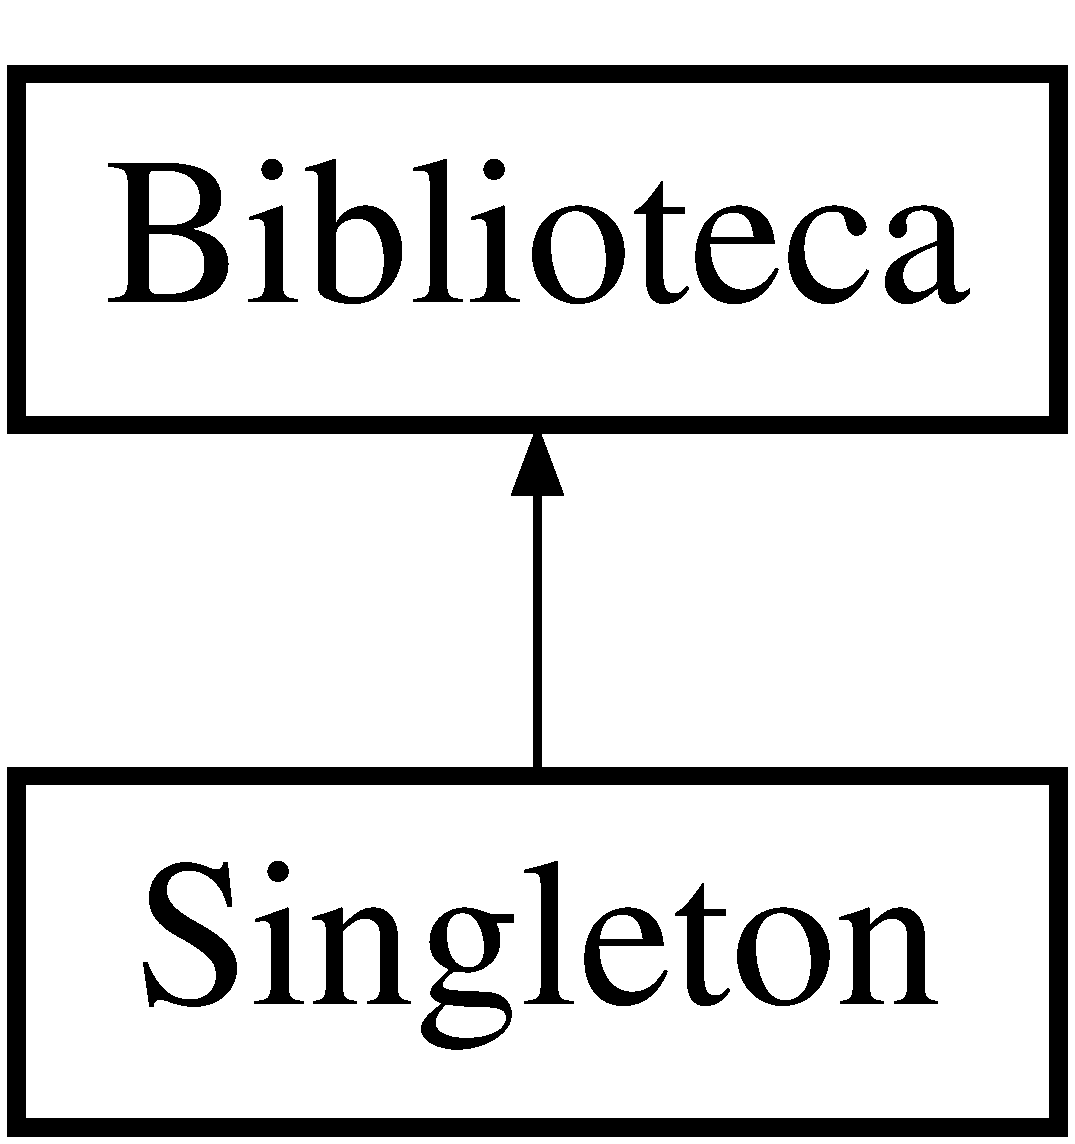
\includegraphics[height=2.000000cm]{class_biblioteca}
\end{center}
\end{figure}
\subsection*{Public Member Functions}
\begin{DoxyCompactItemize}
\item 
\hyperlink{class_biblioteca_a5e12ea4e7a4edb14d210a41708fc1c10}{Biblioteca} ()\hypertarget{class_biblioteca_a5e12ea4e7a4edb14d210a41708fc1c10}{}\label{class_biblioteca_a5e12ea4e7a4edb14d210a41708fc1c10}

\begin{DoxyCompactList}\small\item\em Crea el objeto, carga los datos desde los archivos y elimina sanciones viejas. \end{DoxyCompactList}\item 
\hyperlink{class_biblioteca_ae3f55e8952ed4bdddb82ece48c52f6c0}{$\sim$\+Biblioteca} ()\hypertarget{class_biblioteca_ae3f55e8952ed4bdddb82ece48c52f6c0}{}\label{class_biblioteca_ae3f55e8952ed4bdddb82ece48c52f6c0}

\begin{DoxyCompactList}\small\item\em Destructor, guarda todos los cambios antes de cerrar. \end{DoxyCompactList}\item 
void \hyperlink{class_biblioteca_a183d7a2d3371aa96839af90969a760b4}{Agregar\+Libro} (string titulo, string autores, string editorial, string isbn, string edicion, string tipo, int cod\+Libro, string estado)\hypertarget{class_biblioteca_a183d7a2d3371aa96839af90969a760b4}{}\label{class_biblioteca_a183d7a2d3371aa96839af90969a760b4}

\begin{DoxyCompactList}\small\item\em Agregar un libro. \end{DoxyCompactList}\item 
void \hyperlink{class_biblioteca_a05ea6460b9e61c271ae433f1f9d2b997}{Modificar\+Libro} (string titulo, string autores, string editorial, string isbn, string edicion, string tipo, int cod\+Libro, string estado)\hypertarget{class_biblioteca_a05ea6460b9e61c271ae433f1f9d2b997}{}\label{class_biblioteca_a05ea6460b9e61c271ae433f1f9d2b997}

\begin{DoxyCompactList}\small\item\em Modificar un libro. \end{DoxyCompactList}\item 
void \hyperlink{class_biblioteca_a6936988204544a620644d1130f90e840}{Ocultar\+Libro} (int i)\hypertarget{class_biblioteca_a6936988204544a620644d1130f90e840}{}\label{class_biblioteca_a6936988204544a620644d1130f90e840}

\begin{DoxyCompactList}\small\item\em Oculta un libro de la grilla, funciona como \char`\"{}eliminar\char`\"{} para el usuario. \end{DoxyCompactList}\item 
void \hyperlink{class_biblioteca_acebc2e73ac75bcb3bd42119d71757533}{Agregar\+Lector} (string nombre, string apellido, string dni, string domicilio, string tel, int num\+Lector)\hypertarget{class_biblioteca_acebc2e73ac75bcb3bd42119d71757533}{}\label{class_biblioteca_acebc2e73ac75bcb3bd42119d71757533}

\begin{DoxyCompactList}\small\item\em Agregar un lector. \end{DoxyCompactList}\item 
void \hyperlink{class_biblioteca_a70bf48f7132623ea2f95a3eaf7dd0988}{Modificar\+Lector} (string nombre, string apellido, string dni, string domicilio, string tel, int num\+Lector)\hypertarget{class_biblioteca_a70bf48f7132623ea2f95a3eaf7dd0988}{}\label{class_biblioteca_a70bf48f7132623ea2f95a3eaf7dd0988}

\begin{DoxyCompactList}\small\item\em Modificar un libro. \end{DoxyCompactList}\item 
void \hyperlink{class_biblioteca_a3397bc5478d185f1edfe494b01a7b36f}{Ocultar\+Lector} (int i)\hypertarget{class_biblioteca_a3397bc5478d185f1edfe494b01a7b36f}{}\label{class_biblioteca_a3397bc5478d185f1edfe494b01a7b36f}

\begin{DoxyCompactList}\small\item\em Oculta un lector de la grilla, funciona como \char`\"{}eliminar\char`\"{} para el usuario. \end{DoxyCompactList}\item 
void \hyperlink{class_biblioteca_a636779658541f0f82e0f9505bcb4d66d}{Agregar\+Prestamo} (int numero\+Lector, int codigo\+Libro)\hypertarget{class_biblioteca_a636779658541f0f82e0f9505bcb4d66d}{}\label{class_biblioteca_a636779658541f0f82e0f9505bcb4d66d}

\begin{DoxyCompactList}\small\item\em Agregar un pr�stamo. \end{DoxyCompactList}\item 
int \hyperlink{class_biblioteca_af37ce8c8ef211ab754e70897f3fae0e2}{Eliminar\+Prestamo} (int codigo\+Libro)\hypertarget{class_biblioteca_af37ce8c8ef211ab754e70897f3fae0e2}{}\label{class_biblioteca_af37ce8c8ef211ab754e70897f3fae0e2}

\begin{DoxyCompactList}\small\item\em Eliminar un pr�stamo mediante una devoluci�n \end{DoxyCompactList}\item 
bool \hyperlink{class_biblioteca_a8049c596bc7e22a08c63ed0cf465054d}{Tiene\+Prestamos\+Activos} (int num\+Lector)\hypertarget{class_biblioteca_a8049c596bc7e22a08c63ed0cf465054d}{}\label{class_biblioteca_a8049c596bc7e22a08c63ed0cf465054d}

\begin{DoxyCompactList}\small\item\em Verifica si un lector tiene pr�stamos activos. \end{DoxyCompactList}\item 
void \hyperlink{class_biblioteca_a5f2603f4d430df4e7dfea62e68decebf}{Agregar\+Sancion} (int numero\+Lector, string motivo, int cant\+Dias)\hypertarget{class_biblioteca_a5f2603f4d430df4e7dfea62e68decebf}{}\label{class_biblioteca_a5f2603f4d430df4e7dfea62e68decebf}

\begin{DoxyCompactList}\small\item\em Agregar una sanci�n \end{DoxyCompactList}\item 
void \hyperlink{class_biblioteca_ad0820f1f00b5ccae5e6fc856248579c8}{Eliminar\+Sanciones\+Cumplidas} ()\hypertarget{class_biblioteca_ad0820f1f00b5ccae5e6fc856248579c8}{}\label{class_biblioteca_ad0820f1f00b5ccae5e6fc856248579c8}

\begin{DoxyCompactList}\small\item\em Chequea las sanciones al inicio y elimina las que caducaron. \end{DoxyCompactList}\item 
bool \hyperlink{class_biblioteca_ada5eb122af895870f953d8e9f94f5b18}{Esta\+Sancionado} (int num\+Lector)\hypertarget{class_biblioteca_ada5eb122af895870f953d8e9f94f5b18}{}\label{class_biblioteca_ada5eb122af895870f953d8e9f94f5b18}

\begin{DoxyCompactList}\small\item\em Verifica si un lector esta sancionado. \end{DoxyCompactList}\item 
bool \hyperlink{class_biblioteca_a77e293d2b3fdccd400f2119c47a7dd31}{Guardar} () const \hypertarget{class_biblioteca_a77e293d2b3fdccd400f2119c47a7dd31}{}\label{class_biblioteca_a77e293d2b3fdccd400f2119c47a7dd31}

\begin{DoxyCompactList}\small\item\em Guarda el contenido de los vectores en los archivos. \end{DoxyCompactList}\item 
void \hyperlink{class_biblioteca_a4a2a975acf55cc92b6d61de19e16f2a3}{Escribir\+Log} (string mensaje)\hypertarget{class_biblioteca_a4a2a975acf55cc92b6d61de19e16f2a3}{}\label{class_biblioteca_a4a2a975acf55cc92b6d61de19e16f2a3}

\begin{DoxyCompactList}\small\item\em Guarda en un txt un mensaje con fecha acerca de los eventos ocurridos. \end{DoxyCompactList}\item 
void \hyperlink{class_biblioteca_a30bd3b27cbb2da5e0e4a3c5df1153fee}{Cargar\+Libros\+Desde\+Archivo} ()\hypertarget{class_biblioteca_a30bd3b27cbb2da5e0e4a3c5df1153fee}{}\label{class_biblioteca_a30bd3b27cbb2da5e0e4a3c5df1153fee}

\begin{DoxyCompactList}\small\item\em Carga los libros desde el archivo. \end{DoxyCompactList}\item 
void \hyperlink{class_biblioteca_a22eb1e57a9b2133e1dd32ae735f7c575}{Cargar\+Lectores\+Desde\+Archivo} ()\hypertarget{class_biblioteca_a22eb1e57a9b2133e1dd32ae735f7c575}{}\label{class_biblioteca_a22eb1e57a9b2133e1dd32ae735f7c575}

\begin{DoxyCompactList}\small\item\em Carga los lectores desde el archivo. \end{DoxyCompactList}\item 
void \hyperlink{class_biblioteca_a7e837920c5d48306bc8be3d882975876}{Cargar\+Prestamos\+Desde\+Archivo} ()\hypertarget{class_biblioteca_a7e837920c5d48306bc8be3d882975876}{}\label{class_biblioteca_a7e837920c5d48306bc8be3d882975876}

\begin{DoxyCompactList}\small\item\em Carga los pr�stamos desde el archivo. \end{DoxyCompactList}\item 
void \hyperlink{class_biblioteca_a90b47c3dde2a0d78d2259c265b3e8619}{Cargar\+Sanciones\+Desde\+Archivo} ()\hypertarget{class_biblioteca_a90b47c3dde2a0d78d2259c265b3e8619}{}\label{class_biblioteca_a90b47c3dde2a0d78d2259c265b3e8619}

\begin{DoxyCompactList}\small\item\em Carga las sanciones desde el archivo. \end{DoxyCompactList}\item 
int \hyperlink{class_biblioteca_af10a2bcd13615668374e2fa11cdaeec3}{Buscar\+Titulo} (string parte, int pos\+\_\+desde)\hypertarget{class_biblioteca_af10a2bcd13615668374e2fa11cdaeec3}{}\label{class_biblioteca_af10a2bcd13615668374e2fa11cdaeec3}

\begin{DoxyCompactList}\small\item\em Busqueda por t�tulo en la grilla. \end{DoxyCompactList}\item 
int \hyperlink{class_biblioteca_a71052da035de9de2b358f5913197f7ae}{Buscar\+Apellido\+Y\+Nombre} (string parte, int pos\+\_\+desde)\hypertarget{class_biblioteca_a71052da035de9de2b358f5913197f7ae}{}\label{class_biblioteca_a71052da035de9de2b358f5913197f7ae}

\begin{DoxyCompactList}\small\item\em Busqueda por apellido y nombre en la grilla. \end{DoxyCompactList}\item 
int \hyperlink{class_biblioteca_ac56266e135c24f2bbd99005e508c0e40}{Buscar\+Apellido\+Nombre\+O\+Titulo} (string parte, int pos\+\_\+desde)\hypertarget{class_biblioteca_ac56266e135c24f2bbd99005e508c0e40}{}\label{class_biblioteca_ac56266e135c24f2bbd99005e508c0e40}

\begin{DoxyCompactList}\small\item\em Busqueda por t�tulo, apellido y nombre en la grilla. \end{DoxyCompactList}\item 
int \hyperlink{class_biblioteca_ab6d891537be1eb5e1da58e07e98f00d9}{cant\+Libros} () const \hypertarget{class_biblioteca_ab6d891537be1eb5e1da58e07e98f00d9}{}\label{class_biblioteca_ab6d891537be1eb5e1da58e07e98f00d9}

\begin{DoxyCompactList}\small\item\em Devuelve la cantidad de libros en v\+Libros. \end{DoxyCompactList}\item 
int \hyperlink{class_biblioteca_a84e2cda3c20b42243f42c95f67dc8614}{cant\+Libros\+Activos} () const \hypertarget{class_biblioteca_a84e2cda3c20b42243f42c95f67dc8614}{}\label{class_biblioteca_a84e2cda3c20b42243f42c95f67dc8614}

\begin{DoxyCompactList}\small\item\em Devuelve la cantidad de libros activos en v\+Libros. \end{DoxyCompactList}\item 
int \hyperlink{class_biblioteca_aa3de0dd6e7f6c6b5baba057fcfbd2e7d}{cant\+Lectores} () const \hypertarget{class_biblioteca_aa3de0dd6e7f6c6b5baba057fcfbd2e7d}{}\label{class_biblioteca_aa3de0dd6e7f6c6b5baba057fcfbd2e7d}

\begin{DoxyCompactList}\small\item\em Devuelve la cantidad de lectores en v\+Lectores. \end{DoxyCompactList}\item 
int \hyperlink{class_biblioteca_ae5ed7d4575cc03b3e096dc103ac9fef8}{cant\+Prestamos} () const \hypertarget{class_biblioteca_ae5ed7d4575cc03b3e096dc103ac9fef8}{}\label{class_biblioteca_ae5ed7d4575cc03b3e096dc103ac9fef8}

\begin{DoxyCompactList}\small\item\em Devuelve la cantidad de pr�stamos en v\+Prestamos. \end{DoxyCompactList}\item 
int \hyperlink{class_biblioteca_a8d14fa04a6dc9fcfc2b8e6f0e4d80175}{cant\+Sanciones} () const \hypertarget{class_biblioteca_a8d14fa04a6dc9fcfc2b8e6f0e4d80175}{}\label{class_biblioteca_a8d14fa04a6dc9fcfc2b8e6f0e4d80175}

\begin{DoxyCompactList}\small\item\em Devuelve la cantidad de sanciones en v\+Sanciones. \end{DoxyCompactList}\item 
\hyperlink{class_libro}{Libro} \hyperlink{class_biblioteca_adcc29644a52d7a9abb0a23c4cfff2a64}{Ver\+Libro} (int i) const \hypertarget{class_biblioteca_adcc29644a52d7a9abb0a23c4cfff2a64}{}\label{class_biblioteca_adcc29644a52d7a9abb0a23c4cfff2a64}

\begin{DoxyCompactList}\small\item\em Devuelve un \hyperlink{class_libro}{Libro} de v\+Libros. \end{DoxyCompactList}\item 
\hyperlink{class_lector}{Lector} \hyperlink{class_biblioteca_a0024ccced3594f917f2e3ab34e40865b}{Ver\+Lector} (int i) const \hypertarget{class_biblioteca_a0024ccced3594f917f2e3ab34e40865b}{}\label{class_biblioteca_a0024ccced3594f917f2e3ab34e40865b}

\begin{DoxyCompactList}\small\item\em Devuelve un lector de v\+Lectores. \end{DoxyCompactList}\item 
\hyperlink{class_prestamo}{Prestamo} \hyperlink{class_biblioteca_a5ab75abec4902ea5a4d16be14d2cad80}{Ver\+Prestamo} (int i) const \hypertarget{class_biblioteca_a5ab75abec4902ea5a4d16be14d2cad80}{}\label{class_biblioteca_a5ab75abec4902ea5a4d16be14d2cad80}

\begin{DoxyCompactList}\small\item\em Devuelve un pr�stamo de v\+Prestamos. \end{DoxyCompactList}\item 
\hyperlink{class_sancion}{Sancion} \hyperlink{class_biblioteca_adfe6eb80307519e5dd26f3d5fa90847f}{Ver\+Sancion} (int i) const \hypertarget{class_biblioteca_adfe6eb80307519e5dd26f3d5fa90847f}{}\label{class_biblioteca_adfe6eb80307519e5dd26f3d5fa90847f}

\begin{DoxyCompactList}\small\item\em Devuelve una sanci�n de v\+Sanciones. \end{DoxyCompactList}\end{DoxyCompactItemize}


\subsection{Detailed Description}
Clase contenedora que administra la \hyperlink{class_biblioteca}{Biblioteca}. La misma ser� utilizada mediante un \hyperlink{class_singleton}{Singleton} para evitar m�ltiples instancias. 

Contiene la lista de libros, lectores, pr�stamos y sanciones, y los metodos para guardarlos y buscarlos en sus respectivas pesta�as. Tamb�en contiene los m�todos para agregar, modificar y eliminar elementos. Los datos estan siempre en memoria, y al realizar alguna operaci�n se debe llamar al metodo Guardar para persistir los cambios en los archivos. 

The documentation for this class was generated from the following files\+:\begin{DoxyCompactItemize}
\item 
\hyperlink{_biblioteca_8h}{Biblioteca.\+h}\item 
\hyperlink{_biblioteca_8cpp}{Biblioteca.\+cpp}\end{DoxyCompactItemize}

\hypertarget{class_lector}{}\section{Lector Class Reference}
\label{class_lector}\index{Lector@{Lector}}


Clase que representa a un \hyperlink{class_lector}{Lector}.  




{\ttfamily \#include $<$Lector.\+h$>$}

\subsection*{Public Member Functions}
\begin{DoxyCompactItemize}
\item 
{\bfseries Lector} (string p\+\_\+nombre, string p\+\_\+apellido, string p\+\_\+dni, string p\+\_\+domicilio, string p\+\_\+tel, int p\+\_\+numero\+Lector)\hypertarget{class_lector_a10e8bb8c4814bd977560d4a3703cd3d1}{}\label{class_lector_a10e8bb8c4814bd977560d4a3703cd3d1}

\item 
{\bfseries Lector} (string p\+\_\+nombre, string p\+\_\+apellido, string p\+\_\+dni, string p\+\_\+domicilio, string p\+\_\+tel, int p\+\_\+numero\+Lector, bool p\+\_\+oculto)\hypertarget{class_lector_add83c864d441bf51ceb37811ce262a13}{}\label{class_lector_add83c864d441bf51ceb37811ce262a13}

\item 
string \hyperlink{class_lector_a14e800f96c177ebdb72d1bd38634738b}{Ver\+Nombre} () const \hypertarget{class_lector_a14e800f96c177ebdb72d1bd38634738b}{}\label{class_lector_a14e800f96c177ebdb72d1bd38634738b}

\begin{DoxyCompactList}\small\item\em devuelve los nombres del lector \end{DoxyCompactList}\item 
string \hyperlink{class_lector_a05cd29997ee70e16f4df741d21c73b00}{Ver\+Apellido} () const \hypertarget{class_lector_a05cd29997ee70e16f4df741d21c73b00}{}\label{class_lector_a05cd29997ee70e16f4df741d21c73b00}

\begin{DoxyCompactList}\small\item\em devuelve los apellidos del lector \end{DoxyCompactList}\item 
string \hyperlink{class_lector_a8be5eda068f582079bfaf5e5fb722309}{Ver\+Apellido\+Y\+Nombre} () const \hypertarget{class_lector_a8be5eda068f582079bfaf5e5fb722309}{}\label{class_lector_a8be5eda068f582079bfaf5e5fb722309}

\begin{DoxyCompactList}\small\item\em devuelve el nombre y apellido del lector \end{DoxyCompactList}\item 
string \hyperlink{class_lector_a466f1492383808cff3b83b30609d2ccb}{Ver\+D\+NI} () const \hypertarget{class_lector_a466f1492383808cff3b83b30609d2ccb}{}\label{class_lector_a466f1492383808cff3b83b30609d2ccb}

\begin{DoxyCompactList}\small\item\em devuelve el dni del lector \end{DoxyCompactList}\item 
string \hyperlink{class_lector_ab6fc9174972e8bd4ffc1109fe1fed118}{Ver\+Domicilio} () const \hypertarget{class_lector_ab6fc9174972e8bd4ffc1109fe1fed118}{}\label{class_lector_ab6fc9174972e8bd4ffc1109fe1fed118}

\begin{DoxyCompactList}\small\item\em devuelve el domicilio del lector \end{DoxyCompactList}\item 
string \hyperlink{class_lector_a851ae153496dbb286a7cab621d5515ed}{Ver\+Tel} () const \hypertarget{class_lector_a851ae153496dbb286a7cab621d5515ed}{}\label{class_lector_a851ae153496dbb286a7cab621d5515ed}

\begin{DoxyCompactList}\small\item\em devuelve el telefono del lector \end{DoxyCompactList}\item 
int \hyperlink{class_lector_a60c3944879e5d627eb56f6be1fdf3aa8}{Ver\+Numero\+Lector} () const \hypertarget{class_lector_a60c3944879e5d627eb56f6be1fdf3aa8}{}\label{class_lector_a60c3944879e5d627eb56f6be1fdf3aa8}

\begin{DoxyCompactList}\small\item\em devuelve el n�mero del lector \end{DoxyCompactList}\item 
bool \hyperlink{class_lector_a1f3cf43debd3357af8546e77b9e16fce}{Esta\+Oculto} () const \hypertarget{class_lector_a1f3cf43debd3357af8546e77b9e16fce}{}\label{class_lector_a1f3cf43debd3357af8546e77b9e16fce}

\begin{DoxyCompactList}\small\item\em bool que devuelve si esta oculto/eliminado \end{DoxyCompactList}\item 
void \hyperlink{class_lector_a0ad1cbfb9982083988001709ed4bddc0}{Ocultar} ()\hypertarget{class_lector_a0ad1cbfb9982083988001709ed4bddc0}{}\label{class_lector_a0ad1cbfb9982083988001709ed4bddc0}

\begin{DoxyCompactList}\small\item\em ocultar/eliminar lector \end{DoxyCompactList}\end{DoxyCompactItemize}


\subsection{Detailed Description}
Clase que representa a un \hyperlink{class_lector}{Lector}. 

Contiene los atributos que se guardan de cada lector, metodos para verlos y m�todos para ocultar y ver si estan ocultos 

The documentation for this class was generated from the following files\+:\begin{DoxyCompactItemize}
\item 
\hyperlink{_lector_8h}{Lector.\+h}\item 
\hyperlink{_lector_8cpp}{Lector.\+cpp}\end{DoxyCompactItemize}

\hypertarget{class_libro}{}\section{Libro Class Reference}
\label{class_libro}\index{Libro@{Libro}}


Clase que representa a un \hyperlink{class_libro}{Libro}.  




{\ttfamily \#include $<$Libro.\+h$>$}

\subsection*{Public Member Functions}
\begin{DoxyCompactItemize}
\item 
{\bfseries Libro} (string p\+\_\+titulo, string p\+\_\+autores, string p\+\_\+editorial, string p\+\_\+isbn, string p\+\_\+edicion, int p\+\_\+codigo\+Libro, string p\+\_\+tipo, string p\+\_\+\+Estado)\hypertarget{class_libro_ad73e88d873105db9a67311de1e17f749}{}\label{class_libro_ad73e88d873105db9a67311de1e17f749}

\item 
{\bfseries Libro} (string p\+\_\+titulo, string p\+\_\+autores, string p\+\_\+editorial, string p\+\_\+isbn, string p\+\_\+edicion, int p\+\_\+codigo\+Libro, string p\+\_\+tipo, string p\+\_\+\+Estado, bool p\+\_\+oculto)\hypertarget{class_libro_abffe0deb9e9309ed87e683ee796b4095}{}\label{class_libro_abffe0deb9e9309ed87e683ee796b4095}

\item 
void \hyperlink{class_libro_a212507bd78e7a4bb7b43adb849155c62}{Estado\+Prestado} ()\hypertarget{class_libro_a212507bd78e7a4bb7b43adb849155c62}{}\label{class_libro_a212507bd78e7a4bb7b43adb849155c62}

\begin{DoxyCompactList}\small\item\em cambiar el estado a \char`\"{}\+Prestado\char`\"{} \end{DoxyCompactList}\item 
void \hyperlink{class_libro_ae74afa27b044ada9f30f6e30aedd80c0}{Estado\+Disponible} ()\hypertarget{class_libro_ae74afa27b044ada9f30f6e30aedd80c0}{}\label{class_libro_ae74afa27b044ada9f30f6e30aedd80c0}

\begin{DoxyCompactList}\small\item\em cambiar el estado a \char`\"{}\+Disponible\char`\"{} \end{DoxyCompactList}\item 
void \hyperlink{class_libro_ac20c12b5fe3fc54501136086e67bcc05}{Ocultar} ()\hypertarget{class_libro_ac20c12b5fe3fc54501136086e67bcc05}{}\label{class_libro_ac20c12b5fe3fc54501136086e67bcc05}

\begin{DoxyCompactList}\small\item\em ocultar/eliminar lector \end{DoxyCompactList}\item 
string \hyperlink{class_libro_a13def8d3db34a7863f4c0c88bcb37726}{Ver\+Titulo} () const \hypertarget{class_libro_a13def8d3db34a7863f4c0c88bcb37726}{}\label{class_libro_a13def8d3db34a7863f4c0c88bcb37726}

\begin{DoxyCompactList}\small\item\em devuelve el titulo del \hyperlink{class_libro}{Libro} \end{DoxyCompactList}\item 
string \hyperlink{class_libro_a1ae9e67ab55102827352e482447e2424}{Ver\+Autores} () const \hypertarget{class_libro_a1ae9e67ab55102827352e482447e2424}{}\label{class_libro_a1ae9e67ab55102827352e482447e2424}

\begin{DoxyCompactList}\small\item\em devuelve los autores del \hyperlink{class_libro}{Libro} \end{DoxyCompactList}\item 
string \hyperlink{class_libro_abfd1bc8c6b4fd7c6208ec987467fcb62}{Ver\+Editorial} () const \hypertarget{class_libro_abfd1bc8c6b4fd7c6208ec987467fcb62}{}\label{class_libro_abfd1bc8c6b4fd7c6208ec987467fcb62}

\begin{DoxyCompactList}\small\item\em devuelve la editorial del \hyperlink{class_libro}{Libro} \end{DoxyCompactList}\item 
string \hyperlink{class_libro_a3ed1f24feab829570efd1b196f992e81}{Ver\+I\+S\+BN} () const \hypertarget{class_libro_a3ed1f24feab829570efd1b196f992e81}{}\label{class_libro_a3ed1f24feab829570efd1b196f992e81}

\begin{DoxyCompactList}\small\item\em devuelve el I\+S\+BN del \hyperlink{class_libro}{Libro} \end{DoxyCompactList}\item 
string \hyperlink{class_libro_a725af16e6dc968e66a25aaff90561bc5}{Ver\+Edicion} () const \hypertarget{class_libro_a725af16e6dc968e66a25aaff90561bc5}{}\label{class_libro_a725af16e6dc968e66a25aaff90561bc5}

\begin{DoxyCompactList}\small\item\em devuelve la edici�n del \hyperlink{class_libro}{Libro} \end{DoxyCompactList}\item 
int \hyperlink{class_libro_a76598c9b02e1432bf0ce5e8d6a9b2d25}{Ver\+Codigo\+Libro} () const \hypertarget{class_libro_a76598c9b02e1432bf0ce5e8d6a9b2d25}{}\label{class_libro_a76598c9b02e1432bf0ce5e8d6a9b2d25}

\begin{DoxyCompactList}\small\item\em devuelve el c�digo del \hyperlink{class_libro}{Libro} \end{DoxyCompactList}\item 
string \hyperlink{class_libro_a34fab0359ef8f066abbc267a20377ca9}{Ver\+Tipo} () const \hypertarget{class_libro_a34fab0359ef8f066abbc267a20377ca9}{}\label{class_libro_a34fab0359ef8f066abbc267a20377ca9}

\begin{DoxyCompactList}\small\item\em devuelve el tipo de \hyperlink{class_libro}{Libro} \end{DoxyCompactList}\item 
string \hyperlink{class_libro_ad0fc3222db147beb0eb7df23ced2349a}{Ver\+Estado} () const \hypertarget{class_libro_ad0fc3222db147beb0eb7df23ced2349a}{}\label{class_libro_ad0fc3222db147beb0eb7df23ced2349a}

\begin{DoxyCompactList}\small\item\em devuelve el estado del libro (Prestado o Disponible) \end{DoxyCompactList}\item 
bool \hyperlink{class_libro_a0b23fb23651dfd5f778e6f0dc130b3d6}{Esta\+Disponible} () const \hypertarget{class_libro_a0b23fb23651dfd5f778e6f0dc130b3d6}{}\label{class_libro_a0b23fb23651dfd5f778e6f0dc130b3d6}

\begin{DoxyCompactList}\small\item\em bool que indica si esta Disponible \end{DoxyCompactList}\item 
bool \hyperlink{class_libro_acd838da95a0f0393d1fcd62fc3625d54}{Esta\+Oculto} () const \hypertarget{class_libro_acd838da95a0f0393d1fcd62fc3625d54}{}\label{class_libro_acd838da95a0f0393d1fcd62fc3625d54}

\begin{DoxyCompactList}\small\item\em bool que devuelve si esta oculto/eliminado \end{DoxyCompactList}\end{DoxyCompactItemize}


\subsection{Detailed Description}
Clase que representa a un \hyperlink{class_libro}{Libro}. 

Contiene los atributos que se guardan de cada libro, metodos para verlos y m�todos para ocultar y ver si estan ocultos 

The documentation for this class was generated from the following files\+:\begin{DoxyCompactItemize}
\item 
\hyperlink{_libro_8h}{Libro.\+h}\item 
Libro.\+cpp\end{DoxyCompactItemize}

\hypertarget{classmx_application}{}\section{mx\+Application Class Reference}
\label{classmx_application}\index{mx\+Application@{mx\+Application}}
Inheritance diagram for mx\+Application\+:\begin{figure}[H]
\begin{center}
\leavevmode
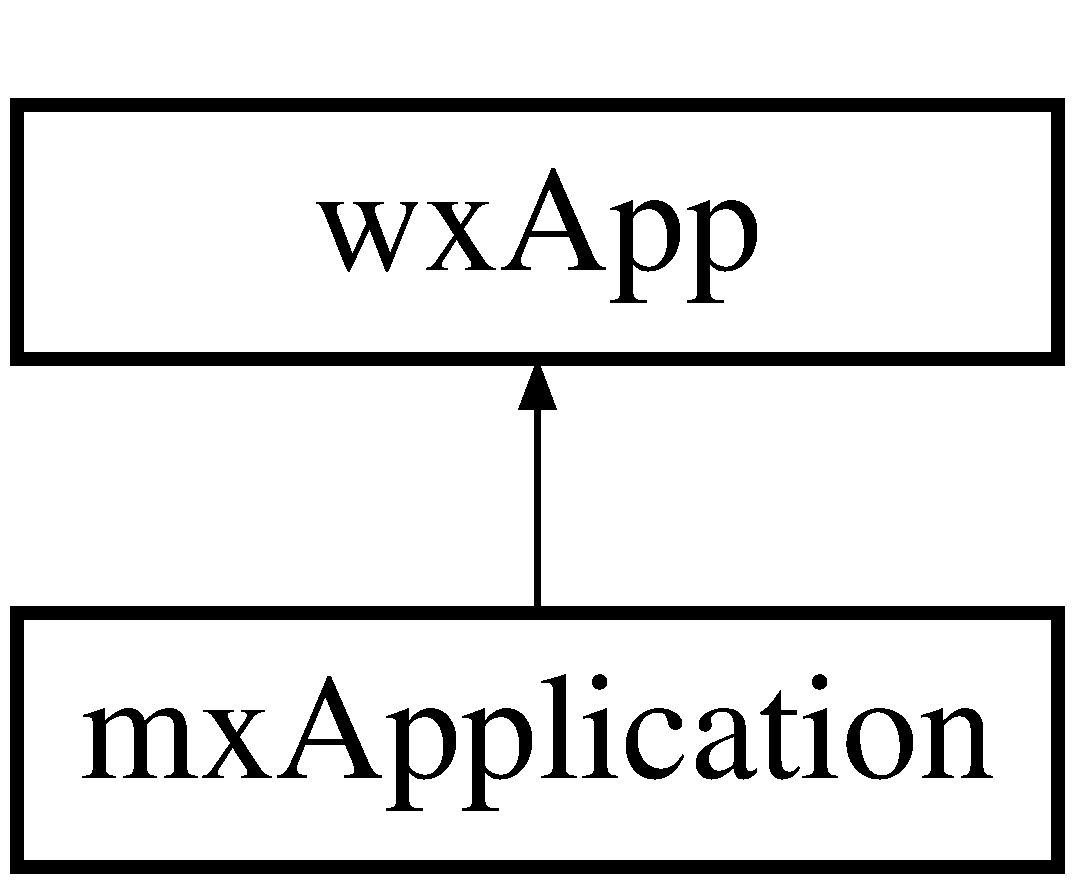
\includegraphics[height=2.000000cm]{classmx_application}
\end{center}
\end{figure}
\subsection*{Public Member Functions}
\begin{DoxyCompactItemize}
\item 
virtual bool {\bfseries On\+Init} ()\hypertarget{classmx_application_a3a3ff4642a63412257a08846ba957834}{}\label{classmx_application_a3a3ff4642a63412257a08846ba957834}

\end{DoxyCompactItemize}


The documentation for this class was generated from the following files\+:\begin{DoxyCompactItemize}
\item 
Application.\+h\item 
Application.\+cpp\end{DoxyCompactItemize}

\hypertarget{class_prestamo}{}\section{Prestamo Class Reference}
\label{class_prestamo}\index{Prestamo@{Prestamo}}


Clase que representa a un \hyperlink{class_prestamo}{Prestamo}.  




{\ttfamily \#include $<$Prestamo.\+h$>$}

\subsection*{Public Member Functions}
\begin{DoxyCompactItemize}
\item 
{\bfseries Prestamo} (int p\+\_\+numero\+Lector, int p\+\_\+\+Codigo\+Libro)\hypertarget{class_prestamo_a33ba3250a9f6b4ae5d576d9a16a89844}{}\label{class_prestamo_a33ba3250a9f6b4ae5d576d9a16a89844}

\item 
{\bfseries Prestamo} (int p\+\_\+numero\+Lector, int p\+\_\+\+Codigo\+Libro, long p\+\_\+\+Fecha\+Desde\+\_\+\+TimeT, long p\+\_\+\+Fecha\+Hasta\+\_\+\+TimeT)\hypertarget{class_prestamo_ac41afdf1f1f38a6bb6df24af368e501e}{}\label{class_prestamo_ac41afdf1f1f38a6bb6df24af368e501e}

\item 
int \hyperlink{class_prestamo_add6781f1deadcbf20560dbb41c137c92}{Ver\+Numero\+Lector\+Prestamo} () const \hypertarget{class_prestamo_add6781f1deadcbf20560dbb41c137c92}{}\label{class_prestamo_add6781f1deadcbf20560dbb41c137c92}

\begin{DoxyCompactList}\small\item\em devuelve el numero del lector del pr�stamo \end{DoxyCompactList}\item 
int \hyperlink{class_prestamo_a5f029996e0154f3f7687ddb7a5b81352}{Ver\+Codigo\+Libro\+Prestamo} () const \hypertarget{class_prestamo_a5f029996e0154f3f7687ddb7a5b81352}{}\label{class_prestamo_a5f029996e0154f3f7687ddb7a5b81352}

\begin{DoxyCompactList}\small\item\em devuelve el c�digo del libro del prestamo \end{DoxyCompactList}\item 
string \hyperlink{class_prestamo_a65bda57e2b4e3f3eb19aba27d1b55fc2}{Ver\+Fecha\+Desde} () const \hypertarget{class_prestamo_a65bda57e2b4e3f3eb19aba27d1b55fc2}{}\label{class_prestamo_a65bda57e2b4e3f3eb19aba27d1b55fc2}

\begin{DoxyCompactList}\small\item\em devuelve la fecha en la que se realiza el prestamo \end{DoxyCompactList}\item 
string \hyperlink{class_prestamo_a39f1750e0f654403eea9c8d6e4512f2c}{Ver\+Fecha\+Hasta} () const \hypertarget{class_prestamo_a39f1750e0f654403eea9c8d6e4512f2c}{}\label{class_prestamo_a39f1750e0f654403eea9c8d6e4512f2c}

\begin{DoxyCompactList}\small\item\em devuelve la fecha limite del plazo del prestamo \end{DoxyCompactList}\item 
long \hyperlink{class_prestamo_a6dc28b655848a976482e3b7803823887}{Ver\+Fecha\+Desde\+\_\+T} () const \hypertarget{class_prestamo_a6dc28b655848a976482e3b7803823887}{}\label{class_prestamo_a6dc28b655848a976482e3b7803823887}

\begin{DoxyCompactList}\small\item\em devuelve la fecha time\+\_\+t en la que se realiza el prestamo \end{DoxyCompactList}\item 
long \hyperlink{class_prestamo_a9c7e4945b40088122afb2a05a51f44a8}{Ver\+Fecha\+Hasta\+\_\+T} () const \hypertarget{class_prestamo_a9c7e4945b40088122afb2a05a51f44a8}{}\label{class_prestamo_a9c7e4945b40088122afb2a05a51f44a8}

\begin{DoxyCompactList}\small\item\em devuelve la fecha time\+\_\+t limite del plazo del prestamo \end{DoxyCompactList}\item 
int \hyperlink{class_prestamo_a48886916cce2dcb07b1de8bc6fc815bc}{Verificar\+Entrega\+A\+Tiempo} () const \hypertarget{class_prestamo_a48886916cce2dcb07b1de8bc6fc815bc}{}\label{class_prestamo_a48886916cce2dcb07b1de8bc6fc815bc}

\begin{DoxyCompactList}\small\item\em devuelve la cantidad de dias tarde que se devolvio el libro \end{DoxyCompactList}\end{DoxyCompactItemize}


\subsection{Detailed Description}
Clase que representa a un \hyperlink{class_prestamo}{Prestamo}. 

Contiene los atributos que se guardan de cada \hyperlink{class_prestamo}{Prestamo}, metodos para verlos y m�todos para verificar las devoluciones a tiempo 

The documentation for this class was generated from the following files\+:\begin{DoxyCompactItemize}
\item 
\hyperlink{_prestamo_8h}{Prestamo.\+h}\item 
Prestamo.\+cpp\end{DoxyCompactItemize}

\hypertarget{structregistro__lector}{}\section{registro\+\_\+lector Struct Reference}
\label{structregistro__lector}\index{registro\+\_\+lector@{registro\+\_\+lector}}


Estructura auxiliar para usar con archivos binarios.  




{\ttfamily \#include $<$Lector.\+h$>$}

\subsection*{Public Attributes}
\begin{DoxyCompactItemize}
\item 
char {\bfseries nombre} \mbox{[}256\mbox{]}\hypertarget{structregistro__lector_a76dbf5af6bfe9a42e8f87d4d624a5a57}{}\label{structregistro__lector_a76dbf5af6bfe9a42e8f87d4d624a5a57}

\item 
char {\bfseries apellido} \mbox{[}256\mbox{]}\hypertarget{structregistro__lector_a12f214e775bed9eebbd30592f9f0e331}{}\label{structregistro__lector_a12f214e775bed9eebbd30592f9f0e331}

\item 
char {\bfseries dni} \mbox{[}256\mbox{]}\hypertarget{structregistro__lector_ace928ead5481bfbfe4b22cdd08cb644b}{}\label{structregistro__lector_ace928ead5481bfbfe4b22cdd08cb644b}

\item 
char {\bfseries domicilio} \mbox{[}256\mbox{]}\hypertarget{structregistro__lector_a302d8795ab5c40a80dfcf025012ef4f5}{}\label{structregistro__lector_a302d8795ab5c40a80dfcf025012ef4f5}

\item 
char {\bfseries tel} \mbox{[}256\mbox{]}\hypertarget{structregistro__lector_adec4e1183f67c388ca79575b6fad7bda}{}\label{structregistro__lector_adec4e1183f67c388ca79575b6fad7bda}

\item 
int {\bfseries numero\+Lector}\hypertarget{structregistro__lector_a44bc703bc8b0910fe5ad579f08b810fa}{}\label{structregistro__lector_a44bc703bc8b0910fe5ad579f08b810fa}

\item 
bool {\bfseries oculto}\hypertarget{structregistro__lector_ab079adb75612f8389b61e0ea2fabbd53}{}\label{structregistro__lector_ab079adb75612f8389b61e0ea2fabbd53}

\end{DoxyCompactItemize}


\subsection{Detailed Description}
Estructura auxiliar para usar con archivos binarios. 

En este struct se guardan los datos para poder llevar strings al archivo 

The documentation for this struct was generated from the following file\+:\begin{DoxyCompactItemize}
\item 
\hyperlink{_lector_8h}{Lector.\+h}\end{DoxyCompactItemize}

\hypertarget{structregistro__libro}{}\section{registro\+\_\+libro Struct Reference}
\label{structregistro__libro}\index{registro\+\_\+libro@{registro\+\_\+libro}}


Estructura auxiliar para usar con archivos binarios.  




{\ttfamily \#include $<$Libro.\+h$>$}

\subsection*{Public Attributes}
\begin{DoxyCompactItemize}
\item 
char {\bfseries titulo} \mbox{[}256\mbox{]}\hypertarget{structregistro__libro_a927d55558f66e31c65d7ae3f4fea2bbd}{}\label{structregistro__libro_a927d55558f66e31c65d7ae3f4fea2bbd}

\item 
char {\bfseries autores} \mbox{[}256\mbox{]}\hypertarget{structregistro__libro_afaabfd498d3abeb76fc8a8e28751a48e}{}\label{structregistro__libro_afaabfd498d3abeb76fc8a8e28751a48e}

\item 
char {\bfseries editorial} \mbox{[}256\mbox{]}\hypertarget{structregistro__libro_a8596876b7b2c3aca7705dd13d32432f2}{}\label{structregistro__libro_a8596876b7b2c3aca7705dd13d32432f2}

\item 
char {\bfseries isbn} \mbox{[}256\mbox{]}\hypertarget{structregistro__libro_ac46fbf13154b202dfdc11150cfca7d18}{}\label{structregistro__libro_ac46fbf13154b202dfdc11150cfca7d18}

\item 
char {\bfseries edicion} \mbox{[}256\mbox{]}\hypertarget{structregistro__libro_a54b8d33355302fb26f3419c39ceac311}{}\label{structregistro__libro_a54b8d33355302fb26f3419c39ceac311}

\item 
int {\bfseries codigo\+Libro}\hypertarget{structregistro__libro_ac310698580322d5c81e42fa966c25402}{}\label{structregistro__libro_ac310698580322d5c81e42fa966c25402}

\item 
char {\bfseries tipo} \mbox{[}256\mbox{]}\hypertarget{structregistro__libro_a69a7484699f12333b188201c16dd8f44}{}\label{structregistro__libro_a69a7484699f12333b188201c16dd8f44}

\item 
char {\bfseries estado} \mbox{[}256\mbox{]}\hypertarget{structregistro__libro_aef2348a0be46badd74226cc985dfaac7}{}\label{structregistro__libro_aef2348a0be46badd74226cc985dfaac7}

\item 
bool {\bfseries oculto}\hypertarget{structregistro__libro_a19773165ae718d16d6f2e5fb17e447f8}{}\label{structregistro__libro_a19773165ae718d16d6f2e5fb17e447f8}

\end{DoxyCompactItemize}


\subsection{Detailed Description}
Estructura auxiliar para usar con archivos binarios. 

En este struct se guardan los datos para poder llevar strings al archivo 

The documentation for this struct was generated from the following file\+:\begin{DoxyCompactItemize}
\item 
\hyperlink{_libro_8h}{Libro.\+h}\end{DoxyCompactItemize}

\hypertarget{structregistro__prestamo}{}\section{registro\+\_\+prestamo Struct Reference}
\label{structregistro__prestamo}\index{registro\+\_\+prestamo@{registro\+\_\+prestamo}}


Estructura auxiliar para usar con archivos binarios.  




{\ttfamily \#include $<$Prestamo.\+h$>$}

\subsection*{Public Attributes}
\begin{DoxyCompactItemize}
\item 
int {\bfseries numero\+Lector}\hypertarget{structregistro__prestamo_a1a1674a7fb97f8be9dbce8ef1cb0b48a}{}\label{structregistro__prestamo_a1a1674a7fb97f8be9dbce8ef1cb0b48a}

\item 
int {\bfseries codigo\+Libro}\hypertarget{structregistro__prestamo_a7cbdec0601ca0b61e2078cdba908a6b6}{}\label{structregistro__prestamo_a7cbdec0601ca0b61e2078cdba908a6b6}

\item 
long {\bfseries fecha\+Desde\+\_\+t}\hypertarget{structregistro__prestamo_a053595fbaa2ff810bf0ce18c7353295f}{}\label{structregistro__prestamo_a053595fbaa2ff810bf0ce18c7353295f}

\item 
long {\bfseries fecha\+Hasta\+\_\+t}\hypertarget{structregistro__prestamo_a05a0ae142fe7455eab7981ab8494c14d}{}\label{structregistro__prestamo_a05a0ae142fe7455eab7981ab8494c14d}

\end{DoxyCompactItemize}


\subsection{Detailed Description}
Estructura auxiliar para usar con archivos binarios. 

En este struct se guardan los datos para poder llevar strings al archivo 

The documentation for this struct was generated from the following file\+:\begin{DoxyCompactItemize}
\item 
\hyperlink{_prestamo_8h}{Prestamo.\+h}\end{DoxyCompactItemize}

\hypertarget{structregistro__sancion}{}\section{registro\+\_\+sancion Struct Reference}
\label{structregistro__sancion}\index{registro\+\_\+sancion@{registro\+\_\+sancion}}


Estructura auxiliar para usar con archivos binarios.  




{\ttfamily \#include $<$Sancion.\+h$>$}

\subsection*{Public Attributes}
\begin{DoxyCompactItemize}
\item 
int {\bfseries numero\+Lector}\hypertarget{structregistro__sancion_ae1f29efe075d22ea7389618475b215a7}{}\label{structregistro__sancion_ae1f29efe075d22ea7389618475b215a7}

\item 
long {\bfseries fecha\+Sancion\+\_\+t}\hypertarget{structregistro__sancion_ac5440b76d468bbfa2008f9aedff53376}{}\label{structregistro__sancion_ac5440b76d468bbfa2008f9aedff53376}

\item 
char {\bfseries motivo} \mbox{[}256\mbox{]}\hypertarget{structregistro__sancion_a8d5afbe87258d4e9ff278b4b1726c74d}{}\label{structregistro__sancion_a8d5afbe87258d4e9ff278b4b1726c74d}

\end{DoxyCompactItemize}


\subsection{Detailed Description}
Estructura auxiliar para usar con archivos binarios. 

En este struct se guardan los datos para poder llevar strings al archivo 

The documentation for this struct was generated from the following file\+:\begin{DoxyCompactItemize}
\item 
\hyperlink{_sancion_8h}{Sancion.\+h}\end{DoxyCompactItemize}

\hypertarget{class_sancion}{}\section{Sancion Class Reference}
\label{class_sancion}\index{Sancion@{Sancion}}


Clase que representa a una \hyperlink{class_sancion}{Sancion}.  




{\ttfamily \#include $<$Sancion.\+h$>$}

\subsection*{Public Member Functions}
\begin{DoxyCompactItemize}
\item 
{\bfseries Sancion} (int p\+\_\+numero\+Lector, long p\+\_\+fecha\+Sancion\+\_\+T, string p\+\_\+motivo)\hypertarget{class_sancion_a8e73bac520a7ee793b0baec4e0e08d30}{}\label{class_sancion_a8e73bac520a7ee793b0baec4e0e08d30}

\item 
void \hyperlink{class_sancion_a0e531cc651ea19edbfaabbed72d35502}{Prolongar\+Sancion} (long cant\+Dias, string p\+\_\+motivo)\hypertarget{class_sancion_a0e531cc651ea19edbfaabbed72d35502}{}\label{class_sancion_a0e531cc651ea19edbfaabbed72d35502}

\begin{DoxyCompactList}\small\item\em prolonga la sancion \end{DoxyCompactList}\item 
int \hyperlink{class_sancion_a3449c1e13babe907c3408670365a7c95}{Ver\+Numero\+Lector} () const \hypertarget{class_sancion_a3449c1e13babe907c3408670365a7c95}{}\label{class_sancion_a3449c1e13babe907c3408670365a7c95}

\begin{DoxyCompactList}\small\item\em devuelve el n�mero de \hyperlink{class_lector}{Lector} \end{DoxyCompactList}\item 
string \hyperlink{class_sancion_a93e86f7ac3457fd3c45a96bd9a5570b5}{Ver\+Fecha\+Sancion} () const \hypertarget{class_sancion_a93e86f7ac3457fd3c45a96bd9a5570b5}{}\label{class_sancion_a93e86f7ac3457fd3c45a96bd9a5570b5}

\begin{DoxyCompactList}\small\item\em devuelve la fecha hasta la cual el lector esta sancionado \end{DoxyCompactList}\item 
long \hyperlink{class_sancion_a3d9fb287cf254017dbce8dc6fcebd611}{Ver\+Fecha\+Sancion\+\_\+T} () const \hypertarget{class_sancion_a3d9fb287cf254017dbce8dc6fcebd611}{}\label{class_sancion_a3d9fb287cf254017dbce8dc6fcebd611}

\begin{DoxyCompactList}\small\item\em devuelve la fecha time\+\_\+t hasta la cual el lector esta sancionado \end{DoxyCompactList}\item 
string \hyperlink{class_sancion_ab300551e670b17197172ccf4c931fea9}{Ver\+Motivo} () const \hypertarget{class_sancion_ab300551e670b17197172ccf4c931fea9}{}\label{class_sancion_ab300551e670b17197172ccf4c931fea9}

\begin{DoxyCompactList}\small\item\em devuelve el motivo por el cual el lector fue sancionado \end{DoxyCompactList}\end{DoxyCompactItemize}


\subsection{Detailed Description}
Clase que representa a una \hyperlink{class_sancion}{Sancion}. 

Contiene los atributos que se guardan de cada \hyperlink{class_sancion}{Sancion}, metodos para verlos y m�todos para prolongar el tiempo de sanci�n 

The documentation for this class was generated from the following files\+:\begin{DoxyCompactItemize}
\item 
\hyperlink{_sancion_8h}{Sancion.\+h}\item 
Sancion.\+cpp\end{DoxyCompactItemize}

\hypertarget{class_singleton}{}\section{Singleton Class Reference}
\label{class_singleton}\index{Singleton@{Singleton}}


Clase \hyperlink{class_singleton}{Singleton} que representa a una \hyperlink{class_biblioteca}{Biblioteca}.  




{\ttfamily \#include $<$Singleton.\+h$>$}

Inheritance diagram for Singleton\+:\begin{figure}[H]
\begin{center}
\leavevmode
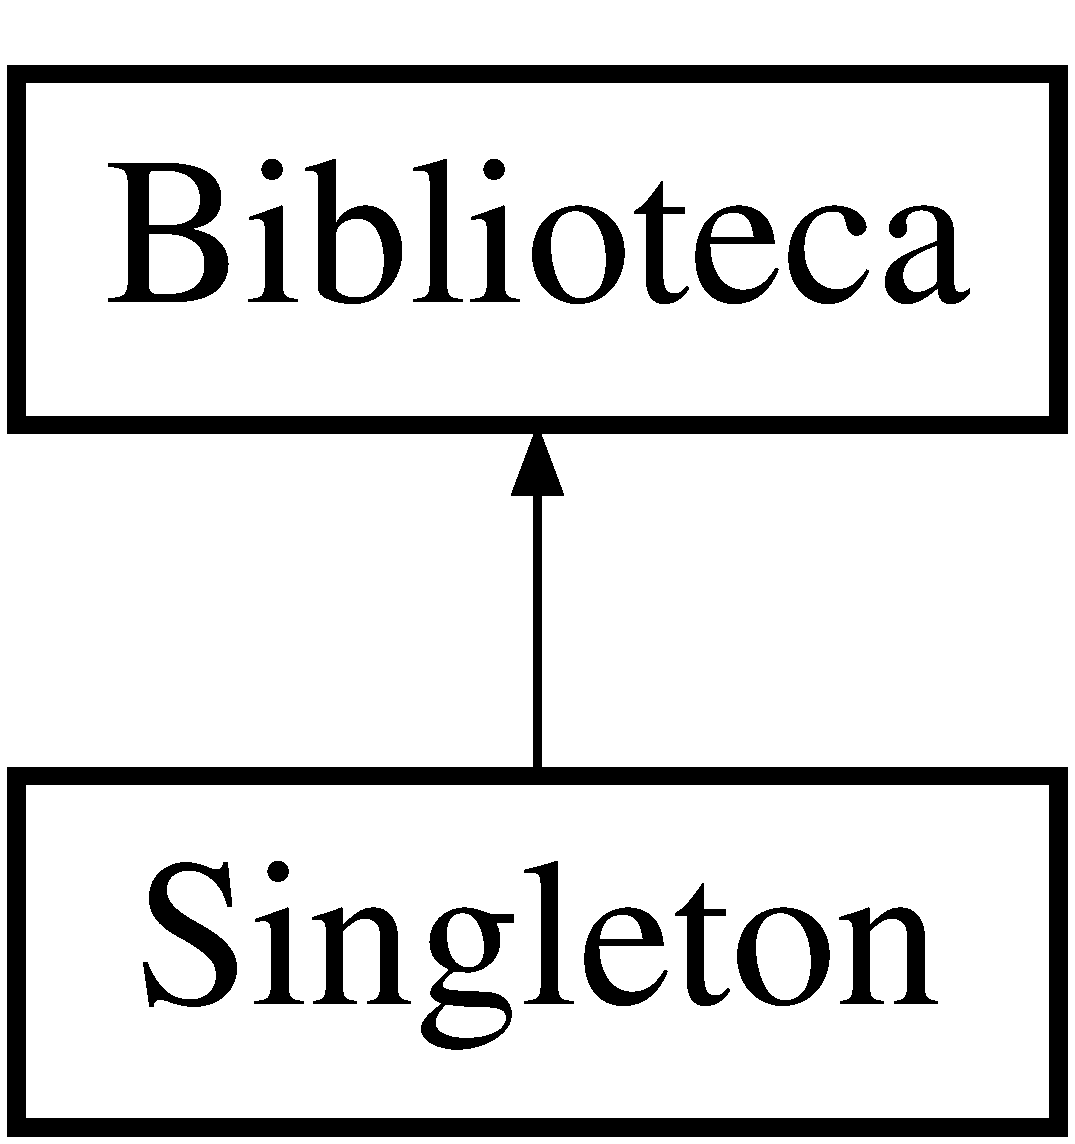
\includegraphics[height=2.000000cm]{class_singleton}
\end{center}
\end{figure}
\subsection*{Static Public Member Functions}
\begin{DoxyCompactItemize}
\item 
static \hyperlink{class_singleton}{Singleton} $\ast$ \hyperlink{class_singleton_af9d918594e37753c7929aced89c01cc8}{Obtener\+Instancia} ()\hypertarget{class_singleton_af9d918594e37753c7929aced89c01cc8}{}\label{class_singleton_af9d918594e37753c7929aced89c01cc8}

\begin{DoxyCompactList}\small\item\em M�todo para obtener la instancia, �nica forma de hacerlo. \end{DoxyCompactList}\end{DoxyCompactItemize}
\subsection*{Additional Inherited Members}


\subsection{Detailed Description}
Clase \hyperlink{class_singleton}{Singleton} que representa a una \hyperlink{class_biblioteca}{Biblioteca}. 

Permite trabajar con una �nica biblioteca para no crear m�ltiples instancias 

The documentation for this class was generated from the following files\+:\begin{DoxyCompactItemize}
\item 
\hyperlink{_singleton_8h}{Singleton.\+h}\item 
\hyperlink{_singleton_8cpp}{Singleton.\+cpp}\end{DoxyCompactItemize}

\hypertarget{class_vagregar_lector}{}\section{Vagregar\+Lector Class Reference}
\label{class_vagregar_lector}\index{Vagregar\+Lector@{Vagregar\+Lector}}
Inheritance diagram for Vagregar\+Lector\+:\begin{figure}[H]
\begin{center}
\leavevmode
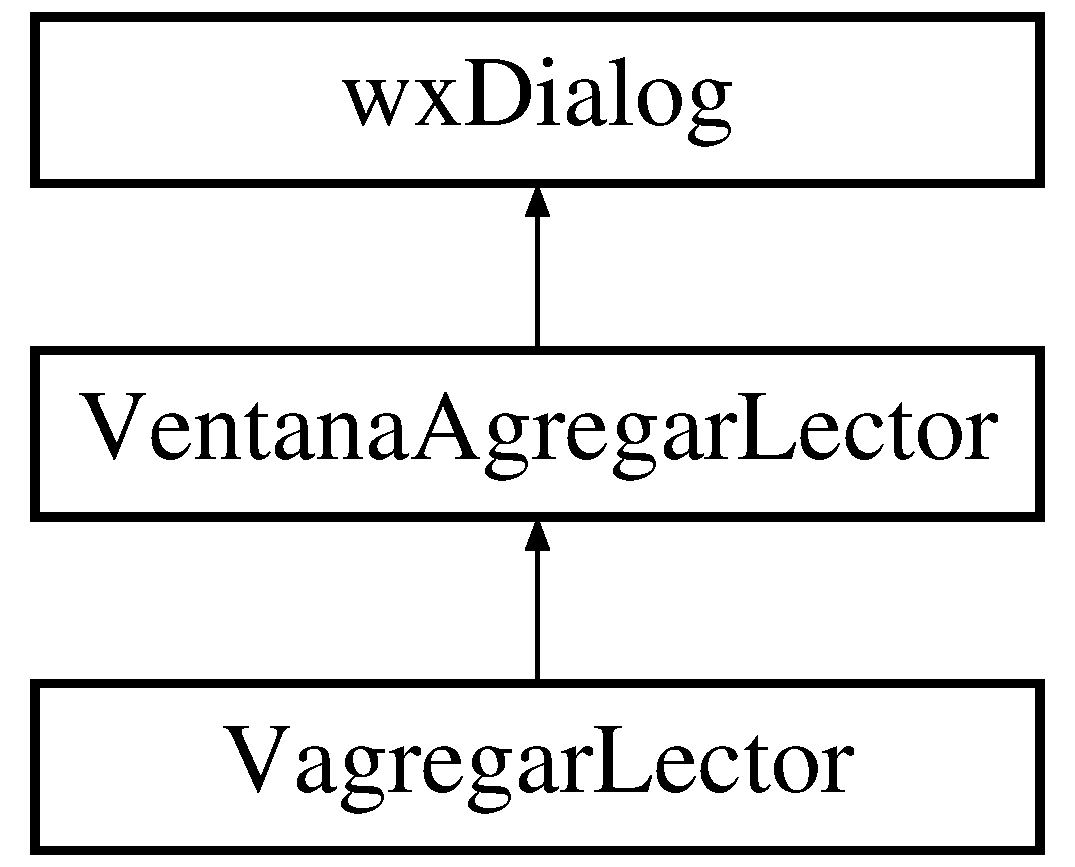
\includegraphics[height=3.000000cm]{class_vagregar_lector}
\end{center}
\end{figure}
\subsection*{Public Member Functions}
\begin{DoxyCompactItemize}
\item 
{\bfseries Vagregar\+Lector} (wx\+Window $\ast$parent=N\+U\+LL)\hypertarget{class_vagregar_lector_abc442f5eb56f5bd5aa2e66db3a21f152}{}\label{class_vagregar_lector_abc442f5eb56f5bd5aa2e66db3a21f152}

\item 
string \hyperlink{class_vagregar_lector_a07c86c6aed75c052619bbae01fa8434c}{Validar\+Datos} ()\hypertarget{class_vagregar_lector_a07c86c6aed75c052619bbae01fa8434c}{}\label{class_vagregar_lector_a07c86c6aed75c052619bbae01fa8434c}

\begin{DoxyCompactList}\small\item\em Valida los datos ingresados. \end{DoxyCompactList}\end{DoxyCompactItemize}
\subsection*{Protected Member Functions}
\begin{DoxyCompactItemize}
\item 
void \hyperlink{class_vagregar_lector_aac8aa34d70f414512439db50aef17151}{Click\+Agregar\+Lector\+Nuevo} (wx\+Command\+Event \&event)\hypertarget{class_vagregar_lector_aac8aa34d70f414512439db50aef17151}{}\label{class_vagregar_lector_aac8aa34d70f414512439db50aef17151}

\begin{DoxyCompactList}\small\item\em Guarda el nuevo dato y cierra la ventana (boton \char`\"{}\+Aceptar\char`\"{});. \end{DoxyCompactList}\item 
void \hyperlink{class_vagregar_lector_a88c689837ca54ff3425bbbb31cde0c7d}{b\+Cancelar\+Agregar\+Lector} (wx\+Command\+Event \&event)\hypertarget{class_vagregar_lector_a88c689837ca54ff3425bbbb31cde0c7d}{}\label{class_vagregar_lector_a88c689837ca54ff3425bbbb31cde0c7d}

\begin{DoxyCompactList}\small\item\em Cierra la ventana sin agregar el nuevo dato (boton \char`\"{}\+Cancelar\char`\"{}) \end{DoxyCompactList}\end{DoxyCompactItemize}
\subsection*{Additional Inherited Members}


The documentation for this class was generated from the following files\+:\begin{DoxyCompactItemize}
\item 
Vagregar\+Lector.\+h\item 
\hyperlink{_vagregar_lector_8cpp}{Vagregar\+Lector.\+cpp}\end{DoxyCompactItemize}

\hypertarget{class_vagregar_libro}{}\section{Vagregar\+Libro Class Reference}
\label{class_vagregar_libro}\index{Vagregar\+Libro@{Vagregar\+Libro}}


Ventana cargar los datos de un nuevo \hyperlink{class_libro}{Libro}.  




{\ttfamily \#include $<$Vagregar\+Libro.\+h$>$}

Inheritance diagram for Vagregar\+Libro\+:\begin{figure}[H]
\begin{center}
\leavevmode
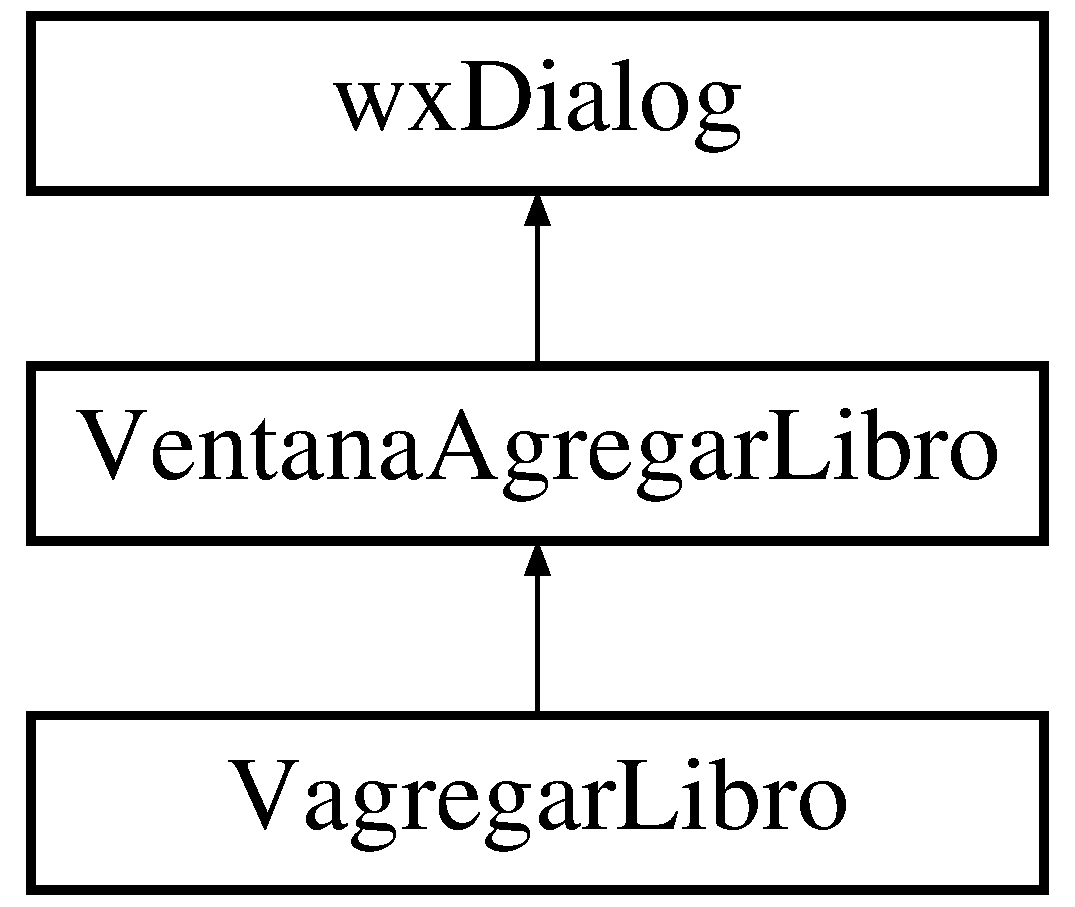
\includegraphics[height=3.000000cm]{class_vagregar_libro}
\end{center}
\end{figure}
\subsection*{Public Member Functions}
\begin{DoxyCompactItemize}
\item 
{\bfseries Vagregar\+Libro} (wx\+Window $\ast$parent=N\+U\+LL)\hypertarget{class_vagregar_libro_a12b4b3824ebe3116d41ed34ffaeb64d9}{}\label{class_vagregar_libro_a12b4b3824ebe3116d41ed34ffaeb64d9}

\item 
string \hyperlink{class_vagregar_libro_a145e90663e920301404c478e932d80de}{Validar\+Datos} ()\hypertarget{class_vagregar_libro_a145e90663e920301404c478e932d80de}{}\label{class_vagregar_libro_a145e90663e920301404c478e932d80de}

\begin{DoxyCompactList}\small\item\em Valida los datos ingresados. \end{DoxyCompactList}\end{DoxyCompactItemize}
\subsection*{Protected Member Functions}
\begin{DoxyCompactItemize}
\item 
void \hyperlink{class_vagregar_libro_a848f2a9686325c645e79a3c27baab56d}{Click\+Agregar\+Libro\+Nuevo} (wx\+Command\+Event \&event)\hypertarget{class_vagregar_libro_a848f2a9686325c645e79a3c27baab56d}{}\label{class_vagregar_libro_a848f2a9686325c645e79a3c27baab56d}

\begin{DoxyCompactList}\small\item\em Guarda el nuevo dato y cierra la ventana (boton \char`\"{}\+Aceptar\char`\"{});. \end{DoxyCompactList}\item 
void \hyperlink{class_vagregar_libro_ac06f67ffcf2968aa6c1412e047b16109}{b\+Cancelar\+Agregar\+Libro} (wx\+Command\+Event \&event)\hypertarget{class_vagregar_libro_ac06f67ffcf2968aa6c1412e047b16109}{}\label{class_vagregar_libro_ac06f67ffcf2968aa6c1412e047b16109}

\begin{DoxyCompactList}\small\item\em Cierra la ventana sin agregar el nuevo dato (boton \char`\"{}\+Cancelar\char`\"{}) \end{DoxyCompactList}\end{DoxyCompactItemize}
\subsection*{Additional Inherited Members}


\subsection{Detailed Description}
Ventana cargar los datos de un nuevo \hyperlink{class_libro}{Libro}. 

The documentation for this class was generated from the following files\+:\begin{DoxyCompactItemize}
\item 
Vagregar\+Libro.\+h\item 
\hyperlink{_vagregar_libro_8cpp}{Vagregar\+Libro.\+cpp}\end{DoxyCompactItemize}

\hypertarget{classv_agregar_prestamo}{}\section{v\+Agregar\+Prestamo Class Reference}
\label{classv_agregar_prestamo}\index{v\+Agregar\+Prestamo@{v\+Agregar\+Prestamo}}


Ventana cargar los datos de un nuevo \hyperlink{class_prestamo}{Prestamo}.  




{\ttfamily \#include $<$v\+Agregar\+Prestamo.\+h$>$}

Inheritance diagram for v\+Agregar\+Prestamo\+:\begin{figure}[H]
\begin{center}
\leavevmode
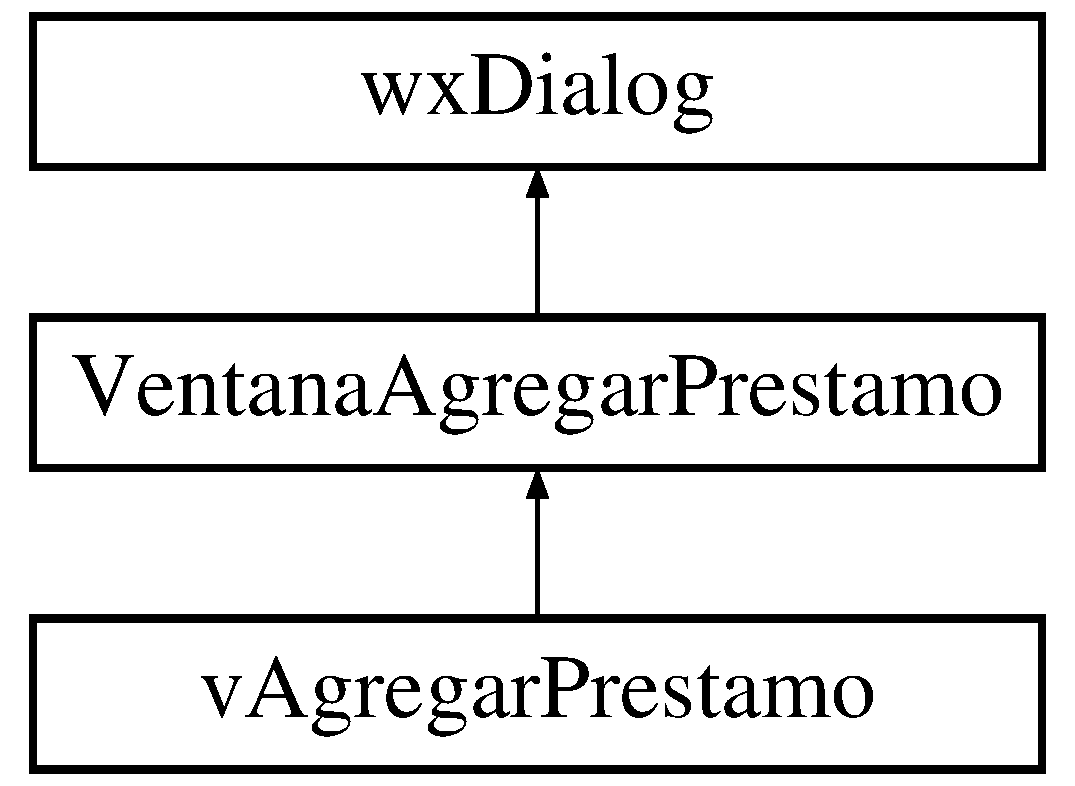
\includegraphics[height=3.000000cm]{classv_agregar_prestamo}
\end{center}
\end{figure}
\subsection*{Public Member Functions}
\begin{DoxyCompactItemize}
\item 
{\bfseries v\+Agregar\+Prestamo} (wx\+Window $\ast$parent=N\+U\+LL)\hypertarget{classv_agregar_prestamo_a515c133ac2af77bce4108930e6dfce5f}{}\label{classv_agregar_prestamo_a515c133ac2af77bce4108930e6dfce5f}

\item 
bool \hyperlink{classv_agregar_prestamo_afc5121b40bfaa0349e9d830aba3f4ff9}{Validar\+Libro} ()\hypertarget{classv_agregar_prestamo_afc5121b40bfaa0349e9d830aba3f4ff9}{}\label{classv_agregar_prestamo_afc5121b40bfaa0349e9d830aba3f4ff9}

\begin{DoxyCompactList}\small\item\em Chequea que se elija un libro y que no este prestado. \end{DoxyCompactList}\item 
bool \hyperlink{classv_agregar_prestamo_ab813531853a031f015f9765d88776cc0}{Validar\+Lector} ()\hypertarget{classv_agregar_prestamo_ab813531853a031f015f9765d88776cc0}{}\label{classv_agregar_prestamo_ab813531853a031f015f9765d88776cc0}

\begin{DoxyCompactList}\small\item\em Chequea que se elija un lector y que no este sancionado. \end{DoxyCompactList}\item 
void \hyperlink{classv_agregar_prestamo_a2eada8be7864922c56543edfcc01741e}{Actualizar\+Label\+Libro} ()\hypertarget{classv_agregar_prestamo_a2eada8be7864922c56543edfcc01741e}{}\label{classv_agregar_prestamo_a2eada8be7864922c56543edfcc01741e}

\begin{DoxyCompactList}\small\item\em Actualiza el label del libro una vez elegido. \end{DoxyCompactList}\item 
void \hyperlink{classv_agregar_prestamo_a96536c490efb539cf025a349c30e570c}{Actualizar\+Label\+Lector} ()\hypertarget{classv_agregar_prestamo_a96536c490efb539cf025a349c30e570c}{}\label{classv_agregar_prestamo_a96536c490efb539cf025a349c30e570c}

\begin{DoxyCompactList}\small\item\em Actualiza el label del lector una vez elegido. \end{DoxyCompactList}\end{DoxyCompactItemize}
\subsection*{Static Public Attributes}
\begin{DoxyCompactItemize}
\item 
static int \hyperlink{classv_agregar_prestamo_a82beccc02f45e937cae62e68b00fba6b}{cod\+Libro} = -\/1\hypertarget{classv_agregar_prestamo_a82beccc02f45e937cae62e68b00fba6b}{}\label{classv_agregar_prestamo_a82beccc02f45e937cae62e68b00fba6b}

\begin{DoxyCompactList}\small\item\em variable estatica del codigo del libro \end{DoxyCompactList}\item 
static int \hyperlink{classv_agregar_prestamo_a8bd94dc889e369f2dfff0f47d9e862d5}{num\+Lector} = -\/1\hypertarget{classv_agregar_prestamo_a8bd94dc889e369f2dfff0f47d9e862d5}{}\label{classv_agregar_prestamo_a8bd94dc889e369f2dfff0f47d9e862d5}

\begin{DoxyCompactList}\small\item\em variable estatica del numero del lector \end{DoxyCompactList}\end{DoxyCompactItemize}
\subsection*{Protected Member Functions}
\begin{DoxyCompactItemize}
\item 
void \hyperlink{classv_agregar_prestamo_a9cb84e29a5ec874fcf1f9c8882131271}{Click\+Aceptar\+Prestamo} (wx\+Command\+Event \&event)\hypertarget{classv_agregar_prestamo_a9cb84e29a5ec874fcf1f9c8882131271}{}\label{classv_agregar_prestamo_a9cb84e29a5ec874fcf1f9c8882131271}

\begin{DoxyCompactList}\small\item\em Guarda el nuevo dato y cierra la ventana (boton \char`\"{}\+Aceptar\char`\"{});. \end{DoxyCompactList}\item 
void \hyperlink{classv_agregar_prestamo_a6c161bb598feb58d8547573dcb4c23a1}{Click\+Cancelar} (wx\+Command\+Event \&event)\hypertarget{classv_agregar_prestamo_a6c161bb598feb58d8547573dcb4c23a1}{}\label{classv_agregar_prestamo_a6c161bb598feb58d8547573dcb4c23a1}

\begin{DoxyCompactList}\small\item\em Cierra la ventana sin agregar el nuevo dato (boton \char`\"{}\+Cancelar\char`\"{}) \end{DoxyCompactList}\item 
void \hyperlink{classv_agregar_prestamo_ad2ad588e036b261a5b03d3f80d30fca0}{Click\+Buscar\+Lector} (wx\+Command\+Event \&event)\hypertarget{classv_agregar_prestamo_ad2ad588e036b261a5b03d3f80d30fca0}{}\label{classv_agregar_prestamo_ad2ad588e036b261a5b03d3f80d30fca0}

\begin{DoxyCompactList}\small\item\em Abre una ventana para elegir el lector del prestamo. \end{DoxyCompactList}\item 
void \hyperlink{classv_agregar_prestamo_a62a63c956c51c7726a88769414ad6046}{Click\+Buscar\+Libro} (wx\+Command\+Event \&event)\hypertarget{classv_agregar_prestamo_a62a63c956c51c7726a88769414ad6046}{}\label{classv_agregar_prestamo_a62a63c956c51c7726a88769414ad6046}

\begin{DoxyCompactList}\small\item\em Abre una ventana para elegir el libro del prestamo. \end{DoxyCompactList}\end{DoxyCompactItemize}
\subsection*{Additional Inherited Members}


\subsection{Detailed Description}
Ventana cargar los datos de un nuevo \hyperlink{class_prestamo}{Prestamo}. 

The documentation for this class was generated from the following files\+:\begin{DoxyCompactItemize}
\item 
v\+Agregar\+Prestamo.\+h\item 
\hyperlink{v_agregar_prestamo_8cpp}{v\+Agregar\+Prestamo.\+cpp}\end{DoxyCompactItemize}

\hypertarget{classv_buscar_lector}{}\section{v\+Buscar\+Lector Class Reference}
\label{classv_buscar_lector}\index{v\+Buscar\+Lector@{v\+Buscar\+Lector}}


Ventana buscar lector para prestamo.  




{\ttfamily \#include $<$v\+Buscar\+Lector.\+h$>$}

Inheritance diagram for v\+Buscar\+Lector\+:\begin{figure}[H]
\begin{center}
\leavevmode
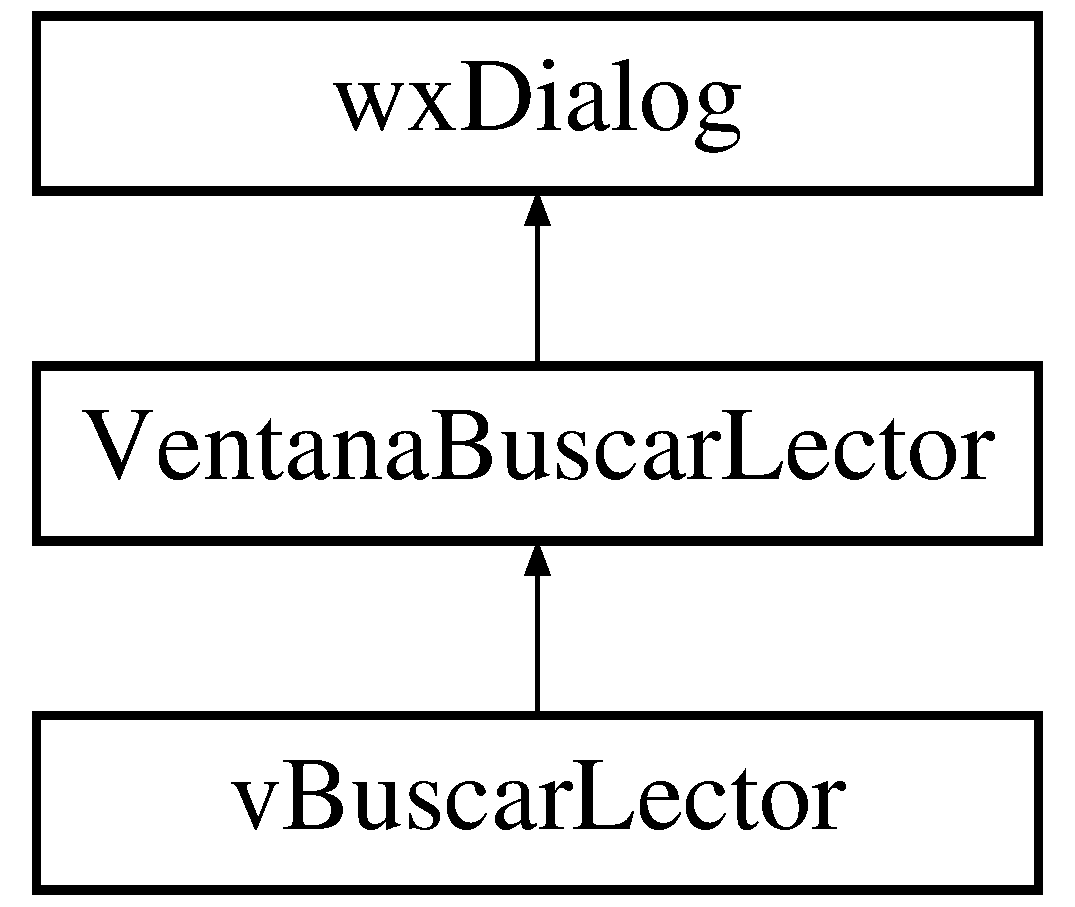
\includegraphics[height=3.000000cm]{classv_buscar_lector}
\end{center}
\end{figure}
\subsection*{Public Member Functions}
\begin{DoxyCompactItemize}
\item 
\hyperlink{classv_buscar_lector_aa7c55a55519cd7a80bac7eeeba2bd1f2}{v\+Buscar\+Lector} (wx\+Window $\ast$parent=N\+U\+LL)\hypertarget{classv_buscar_lector_aa7c55a55519cd7a80bac7eeeba2bd1f2}{}\label{classv_buscar_lector_aa7c55a55519cd7a80bac7eeeba2bd1f2}

\begin{DoxyCompactList}\small\item\em Implementa los metodos para buscar lector para prestamo. \end{DoxyCompactList}\item 
void \hyperlink{classv_buscar_lector_a3d7e7d73baab3bac2e7d5468409fd3bc}{Cargar\+Fila\+Lectores} (int i)\hypertarget{classv_buscar_lector_a3d7e7d73baab3bac2e7d5468409fd3bc}{}\label{classv_buscar_lector_a3d7e7d73baab3bac2e7d5468409fd3bc}

\begin{DoxyCompactList}\small\item\em Carga los datos en la grilla. \end{DoxyCompactList}\end{DoxyCompactItemize}
\subsection*{Protected Member Functions}
\begin{DoxyCompactItemize}
\item 
void \hyperlink{classv_buscar_lector_af4f26568235cb509e3dda02aa9acfb93}{Click\+Busqueda\+Por\+Nombre} (wx\+Command\+Event \&event)\hypertarget{classv_buscar_lector_af4f26568235cb509e3dda02aa9acfb93}{}\label{classv_buscar_lector_af4f26568235cb509e3dda02aa9acfb93}

\begin{DoxyCompactList}\small\item\em Busca por nombre segun la cadena ingresada. \end{DoxyCompactList}\item 
void \hyperlink{classv_buscar_lector_a2049afb7b506b281493435a9f992f972}{D\+Click\+Aceptar\+Lector\+Prestamo} (wx\+Grid\+Event \&event)\hypertarget{classv_buscar_lector_a2049afb7b506b281493435a9f992f972}{}\label{classv_buscar_lector_a2049afb7b506b281493435a9f992f972}

\begin{DoxyCompactList}\small\item\em Guarda el nuevo dato y cierra la ventana (boton \char`\"{}\+Aceptar\char`\"{});. \end{DoxyCompactList}\end{DoxyCompactItemize}
\subsection*{Additional Inherited Members}


\subsection{Detailed Description}
Ventana buscar lector para prestamo. 

The documentation for this class was generated from the following files\+:\begin{DoxyCompactItemize}
\item 
v\+Buscar\+Lector.\+h\item 
v\+Buscar\+Lector.\+cpp\end{DoxyCompactItemize}

\hypertarget{classv_buscar_libro}{}\section{v\+Buscar\+Libro Class Reference}
\label{classv_buscar_libro}\index{v\+Buscar\+Libro@{v\+Buscar\+Libro}}


Ventana buscar libro para prestamo.  




{\ttfamily \#include $<$v\+Buscar\+Libro.\+h$>$}

Inheritance diagram for v\+Buscar\+Libro\+:\begin{figure}[H]
\begin{center}
\leavevmode
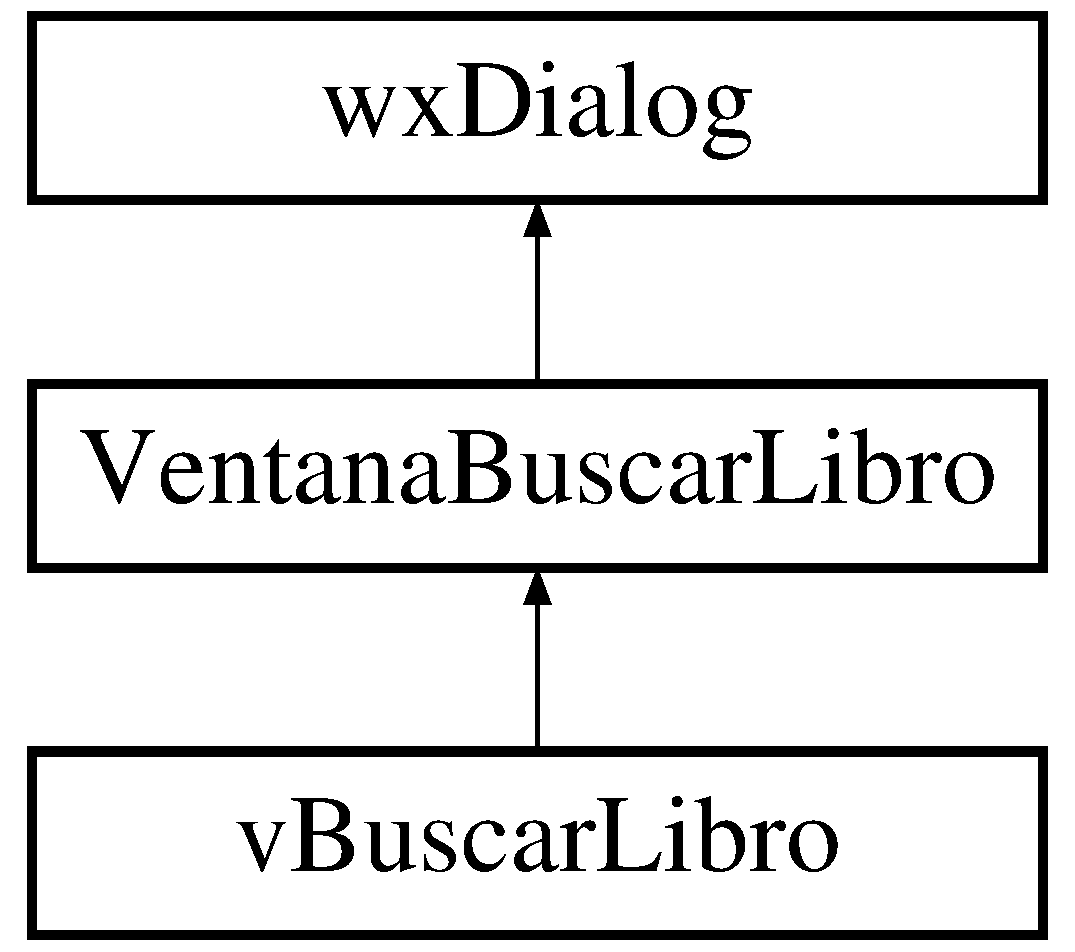
\includegraphics[height=3.000000cm]{classv_buscar_libro}
\end{center}
\end{figure}
\subsection*{Public Member Functions}
\begin{DoxyCompactItemize}
\item 
\hyperlink{classv_buscar_libro_aed0b47d6d8b0b840c4b3c16b80f80957}{v\+Buscar\+Libro} (wx\+Window $\ast$parent=N\+U\+LL)\hypertarget{classv_buscar_libro_aed0b47d6d8b0b840c4b3c16b80f80957}{}\label{classv_buscar_libro_aed0b47d6d8b0b840c4b3c16b80f80957}

\begin{DoxyCompactList}\small\item\em Implementa los metodos para buscar libro para prestamo. \end{DoxyCompactList}\item 
void \hyperlink{classv_buscar_libro_a90c6d94b423998ae8853f97f6f3852c7}{Cargar\+Fila\+Libros} (int i)\hypertarget{classv_buscar_libro_a90c6d94b423998ae8853f97f6f3852c7}{}\label{classv_buscar_libro_a90c6d94b423998ae8853f97f6f3852c7}

\begin{DoxyCompactList}\small\item\em Carga los datos en la grilla. \end{DoxyCompactList}\end{DoxyCompactItemize}
\subsection*{Protected Member Functions}
\begin{DoxyCompactItemize}
\item 
void \hyperlink{classv_buscar_libro_aa002a4d4676ad63725db1bb097f1dbf8}{D\+Click\+Aceptar\+Libro\+Prestamo} (wx\+Grid\+Event \&event)\hypertarget{classv_buscar_libro_aa002a4d4676ad63725db1bb097f1dbf8}{}\label{classv_buscar_libro_aa002a4d4676ad63725db1bb097f1dbf8}

\begin{DoxyCompactList}\small\item\em Elige un libro y cierra la ventana (doble click) \end{DoxyCompactList}\item 
void \hyperlink{classv_buscar_libro_a45e99845766164470d4ab1a2ba79377f}{Click\+Busqueda\+Por\+Titulo} (wx\+Command\+Event \&event)\hypertarget{classv_buscar_libro_a45e99845766164470d4ab1a2ba79377f}{}\label{classv_buscar_libro_a45e99845766164470d4ab1a2ba79377f}

\begin{DoxyCompactList}\small\item\em Busca por titulo segun la cadena ingresada. \end{DoxyCompactList}\end{DoxyCompactItemize}
\subsection*{Additional Inherited Members}


\subsection{Detailed Description}
Ventana buscar libro para prestamo. 

The documentation for this class was generated from the following files\+:\begin{DoxyCompactItemize}
\item 
v\+Buscar\+Libro.\+h\item 
v\+Buscar\+Libro.\+cpp\end{DoxyCompactItemize}

\hypertarget{class_ventana_agregar_lector}{}\section{Ventana\+Agregar\+Lector Class Reference}
\label{class_ventana_agregar_lector}\index{Ventana\+Agregar\+Lector@{Ventana\+Agregar\+Lector}}


Class \hyperlink{class_ventana_agregar_lector}{Ventana\+Agregar\+Lector}.  




{\ttfamily \#include $<$Ventanas.\+h$>$}

Inheritance diagram for Ventana\+Agregar\+Lector\+:\begin{figure}[H]
\begin{center}
\leavevmode
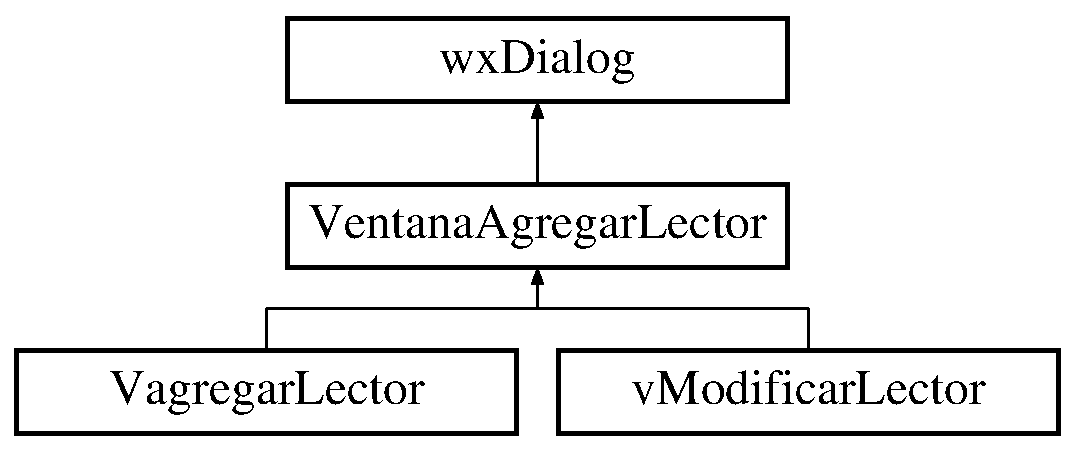
\includegraphics[height=3.000000cm]{class_ventana_agregar_lector}
\end{center}
\end{figure}
\subsection*{Public Member Functions}
\begin{DoxyCompactItemize}
\item 
{\bfseries Ventana\+Agregar\+Lector} (wx\+Window $\ast$parent, wx\+Window\+ID id=wx\+I\+D\+\_\+\+A\+NY, const wx\+String \&title=wxT(\char`\"{}Agregar \hyperlink{class_lector}{Lector}\char`\"{}), const wx\+Point \&pos=wx\+Default\+Position, const wx\+Size \&size=wx\+Size(350, 281), long style=wx\+D\+E\+F\+A\+U\+L\+T\+\_\+\+D\+I\+A\+L\+O\+G\+\_\+\+S\+T\+Y\+LE)\hypertarget{class_ventana_agregar_lector_a22bf15c810d43d286a336c1e3324f75d}{}\label{class_ventana_agregar_lector_a22bf15c810d43d286a336c1e3324f75d}

\end{DoxyCompactItemize}
\subsection*{Protected Member Functions}
\begin{DoxyCompactItemize}
\item 
virtual void {\bfseries b\+Cancelar\+Agregar\+Lector} (wx\+Command\+Event \&event)\hypertarget{class_ventana_agregar_lector_a2e95e648484392e1bf99b03b3ec46e41}{}\label{class_ventana_agregar_lector_a2e95e648484392e1bf99b03b3ec46e41}

\item 
virtual void {\bfseries Click\+Agregar\+Lector\+Nuevo} (wx\+Command\+Event \&event)\hypertarget{class_ventana_agregar_lector_ac1ceb71d63048cbd1b5d856b6b65ae2e}{}\label{class_ventana_agregar_lector_ac1ceb71d63048cbd1b5d856b6b65ae2e}

\end{DoxyCompactItemize}
\subsection*{Protected Attributes}
\begin{DoxyCompactItemize}
\item 
wx\+Static\+Text $\ast$ {\bfseries m\+\_\+static\+Text13}\hypertarget{class_ventana_agregar_lector_a12c54b024085482f6004e4eb4c0449d5}{}\label{class_ventana_agregar_lector_a12c54b024085482f6004e4eb4c0449d5}

\item 
wx\+Text\+Ctrl $\ast$ {\bfseries t\+Nombre}\hypertarget{class_ventana_agregar_lector_a8fbcbd2c77854dd84f5e74209e1cef98}{}\label{class_ventana_agregar_lector_a8fbcbd2c77854dd84f5e74209e1cef98}

\item 
wx\+Static\+Text $\ast$ {\bfseries m\+\_\+static\+Text14}\hypertarget{class_ventana_agregar_lector_a728086583637cd8a34e162de6d0136fe}{}\label{class_ventana_agregar_lector_a728086583637cd8a34e162de6d0136fe}

\item 
wx\+Text\+Ctrl $\ast$ {\bfseries t\+Apellido}\hypertarget{class_ventana_agregar_lector_a9443becc8fb3b8325261e0d27cc64365}{}\label{class_ventana_agregar_lector_a9443becc8fb3b8325261e0d27cc64365}

\item 
wx\+Static\+Text $\ast$ {\bfseries m\+\_\+static\+Text15}\hypertarget{class_ventana_agregar_lector_a4bdc7954166e29ac018d43f9ff8cb47c}{}\label{class_ventana_agregar_lector_a4bdc7954166e29ac018d43f9ff8cb47c}

\item 
wx\+Text\+Ctrl $\ast$ {\bfseries t\+D\+NI}\hypertarget{class_ventana_agregar_lector_a66eb87ced112fbbebf13b0fe9442a753}{}\label{class_ventana_agregar_lector_a66eb87ced112fbbebf13b0fe9442a753}

\item 
wx\+Static\+Text $\ast$ {\bfseries m\+\_\+static\+Text16}\hypertarget{class_ventana_agregar_lector_ac8ba84c88d7a95a93f6868cd3748fa34}{}\label{class_ventana_agregar_lector_ac8ba84c88d7a95a93f6868cd3748fa34}

\item 
wx\+Text\+Ctrl $\ast$ {\bfseries t\+Domicilio}\hypertarget{class_ventana_agregar_lector_a81aa08e4ab58c1b84d936ab2ace2d511}{}\label{class_ventana_agregar_lector_a81aa08e4ab58c1b84d936ab2ace2d511}

\item 
wx\+Static\+Text $\ast$ {\bfseries m\+\_\+static\+Text17}\hypertarget{class_ventana_agregar_lector_a08acf07b63e9760b8b6634e65237cd73}{}\label{class_ventana_agregar_lector_a08acf07b63e9760b8b6634e65237cd73}

\item 
wx\+Text\+Ctrl $\ast$ {\bfseries t\+Telefono}\hypertarget{class_ventana_agregar_lector_ab615ccb040225be5e72495c1dcb75822}{}\label{class_ventana_agregar_lector_ab615ccb040225be5e72495c1dcb75822}

\item 
wx\+Button $\ast$ {\bfseries b\+Cancelar}\hypertarget{class_ventana_agregar_lector_a9e73416a6f984d5f2aa6776665543ee4}{}\label{class_ventana_agregar_lector_a9e73416a6f984d5f2aa6776665543ee4}

\item 
wx\+Button $\ast$ {\bfseries b\+Agregar\+Lector}\hypertarget{class_ventana_agregar_lector_a095ba7bf5353c4fbd8d9fca5df2db5aa}{}\label{class_ventana_agregar_lector_a095ba7bf5353c4fbd8d9fca5df2db5aa}

\end{DoxyCompactItemize}


\subsection{Detailed Description}
Class \hyperlink{class_ventana_agregar_lector}{Ventana\+Agregar\+Lector}. 

The documentation for this class was generated from the following files\+:\begin{DoxyCompactItemize}
\item 
Ventanas.\+h\item 
Ventanas.\+cpp\end{DoxyCompactItemize}

\hypertarget{class_ventana_agregar_libro}{}\section{Ventana\+Agregar\+Libro Class Reference}
\label{class_ventana_agregar_libro}\index{Ventana\+Agregar\+Libro@{Ventana\+Agregar\+Libro}}


Class \hyperlink{class_ventana_agregar_libro}{Ventana\+Agregar\+Libro}.  




{\ttfamily \#include $<$Ventanas.\+h$>$}

Inheritance diagram for Ventana\+Agregar\+Libro\+:\begin{figure}[H]
\begin{center}
\leavevmode
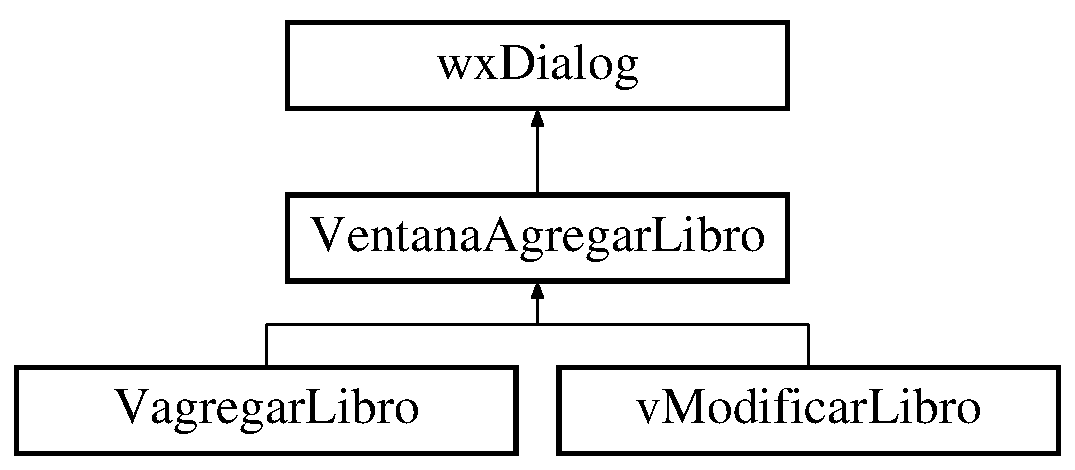
\includegraphics[height=3.000000cm]{class_ventana_agregar_libro}
\end{center}
\end{figure}
\subsection*{Public Member Functions}
\begin{DoxyCompactItemize}
\item 
{\bfseries Ventana\+Agregar\+Libro} (wx\+Window $\ast$parent, wx\+Window\+ID id=wx\+I\+D\+\_\+\+A\+NY, const wx\+String \&title=wxT(\char`\"{}Libro\char`\"{}), const wx\+Point \&pos=wx\+Default\+Position, const wx\+Size \&size=wx\+Size(350, 281), long style=wx\+D\+E\+F\+A\+U\+L\+T\+\_\+\+D\+I\+A\+L\+O\+G\+\_\+\+S\+T\+Y\+LE)\hypertarget{class_ventana_agregar_libro_abe337ae1ac04d4485b962dd057a0c309}{}\label{class_ventana_agregar_libro_abe337ae1ac04d4485b962dd057a0c309}

\end{DoxyCompactItemize}
\subsection*{Protected Member Functions}
\begin{DoxyCompactItemize}
\item 
virtual void {\bfseries b\+Cancelar\+Agregar\+Libro} (wx\+Command\+Event \&event)\hypertarget{class_ventana_agregar_libro_a76c200b1b15ae50c687ef033a193749d}{}\label{class_ventana_agregar_libro_a76c200b1b15ae50c687ef033a193749d}

\item 
virtual void {\bfseries Click\+Agregar\+Libro\+Nuevo} (wx\+Command\+Event \&event)\hypertarget{class_ventana_agregar_libro_a572f8a6b380f8b79810e7198978d4ab1}{}\label{class_ventana_agregar_libro_a572f8a6b380f8b79810e7198978d4ab1}

\end{DoxyCompactItemize}
\subsection*{Protected Attributes}
\begin{DoxyCompactItemize}
\item 
wx\+Static\+Text $\ast$ {\bfseries m\+\_\+static\+Text13}\hypertarget{class_ventana_agregar_libro_a61157e1dee1919687f394583302f1a1a}{}\label{class_ventana_agregar_libro_a61157e1dee1919687f394583302f1a1a}

\item 
wx\+Text\+Ctrl $\ast$ {\bfseries t\+Titulo}\hypertarget{class_ventana_agregar_libro_a69cb961eb7f2e0c25b951e492e3ffb42}{}\label{class_ventana_agregar_libro_a69cb961eb7f2e0c25b951e492e3ffb42}

\item 
wx\+Static\+Text $\ast$ {\bfseries m\+\_\+static\+Text14}\hypertarget{class_ventana_agregar_libro_a363639adfb8f5f2e80836d47c4b70587}{}\label{class_ventana_agregar_libro_a363639adfb8f5f2e80836d47c4b70587}

\item 
wx\+Text\+Ctrl $\ast$ {\bfseries t\+Autor}\hypertarget{class_ventana_agregar_libro_a1cf09e738d9ef609fdc5ce4c355e9cd3}{}\label{class_ventana_agregar_libro_a1cf09e738d9ef609fdc5ce4c355e9cd3}

\item 
wx\+Static\+Text $\ast$ {\bfseries m\+\_\+static\+Text15}\hypertarget{class_ventana_agregar_libro_ac645772b8212e9c096075db14e15f7ac}{}\label{class_ventana_agregar_libro_ac645772b8212e9c096075db14e15f7ac}

\item 
wx\+Text\+Ctrl $\ast$ {\bfseries t\+Editorial}\hypertarget{class_ventana_agregar_libro_af7802bba10855774fa78b62f10a35263}{}\label{class_ventana_agregar_libro_af7802bba10855774fa78b62f10a35263}

\item 
wx\+Static\+Text $\ast$ {\bfseries m\+\_\+static\+Text16}\hypertarget{class_ventana_agregar_libro_af90987acc12ed974e633ff33dce0f10f}{}\label{class_ventana_agregar_libro_af90987acc12ed974e633ff33dce0f10f}

\item 
wx\+Text\+Ctrl $\ast$ {\bfseries t\+I\+S\+BN}\hypertarget{class_ventana_agregar_libro_ab268fc40618913045e15ed7a663c8e68}{}\label{class_ventana_agregar_libro_ab268fc40618913045e15ed7a663c8e68}

\item 
wx\+Static\+Text $\ast$ {\bfseries m\+\_\+static\+Text17}\hypertarget{class_ventana_agregar_libro_a4a82374d54bd0f25d845eb5d3da95666}{}\label{class_ventana_agregar_libro_a4a82374d54bd0f25d845eb5d3da95666}

\item 
wx\+Text\+Ctrl $\ast$ {\bfseries t\+Edicion}\hypertarget{class_ventana_agregar_libro_a3bf5ea3a402525b7085689bf4e0afae5}{}\label{class_ventana_agregar_libro_a3bf5ea3a402525b7085689bf4e0afae5}

\item 
wx\+Static\+Text $\ast$ {\bfseries m\+\_\+static\+Text18}\hypertarget{class_ventana_agregar_libro_acff559e7bf09b29813593bc142daa934}{}\label{class_ventana_agregar_libro_acff559e7bf09b29813593bc142daa934}

\item 
wx\+Text\+Ctrl $\ast$ {\bfseries t\+Tipo}\hypertarget{class_ventana_agregar_libro_aa210a8acb799094bb8476afe4c9e1ae8}{}\label{class_ventana_agregar_libro_aa210a8acb799094bb8476afe4c9e1ae8}

\item 
wx\+Button $\ast$ {\bfseries b\+Cancelar}\hypertarget{class_ventana_agregar_libro_ad51b9dbf930da1a35e939c597558aca5}{}\label{class_ventana_agregar_libro_ad51b9dbf930da1a35e939c597558aca5}

\item 
wx\+Button $\ast$ {\bfseries b\+Agregar\+Libro}\hypertarget{class_ventana_agregar_libro_aced204df0393cdc66d39ec9eccbd579f}{}\label{class_ventana_agregar_libro_aced204df0393cdc66d39ec9eccbd579f}

\end{DoxyCompactItemize}


\subsection{Detailed Description}
Class \hyperlink{class_ventana_agregar_libro}{Ventana\+Agregar\+Libro}. 

The documentation for this class was generated from the following files\+:\begin{DoxyCompactItemize}
\item 
Ventanas.\+h\item 
Ventanas.\+cpp\end{DoxyCompactItemize}

\hypertarget{class_ventana_agregar_prestamo}{}\section{Ventana\+Agregar\+Prestamo Class Reference}
\label{class_ventana_agregar_prestamo}\index{Ventana\+Agregar\+Prestamo@{Ventana\+Agregar\+Prestamo}}


Class \hyperlink{class_ventana_agregar_prestamo}{Ventana\+Agregar\+Prestamo}.  




{\ttfamily \#include $<$Ventanas.\+h$>$}

Inheritance diagram for Ventana\+Agregar\+Prestamo\+:\begin{figure}[H]
\begin{center}
\leavevmode
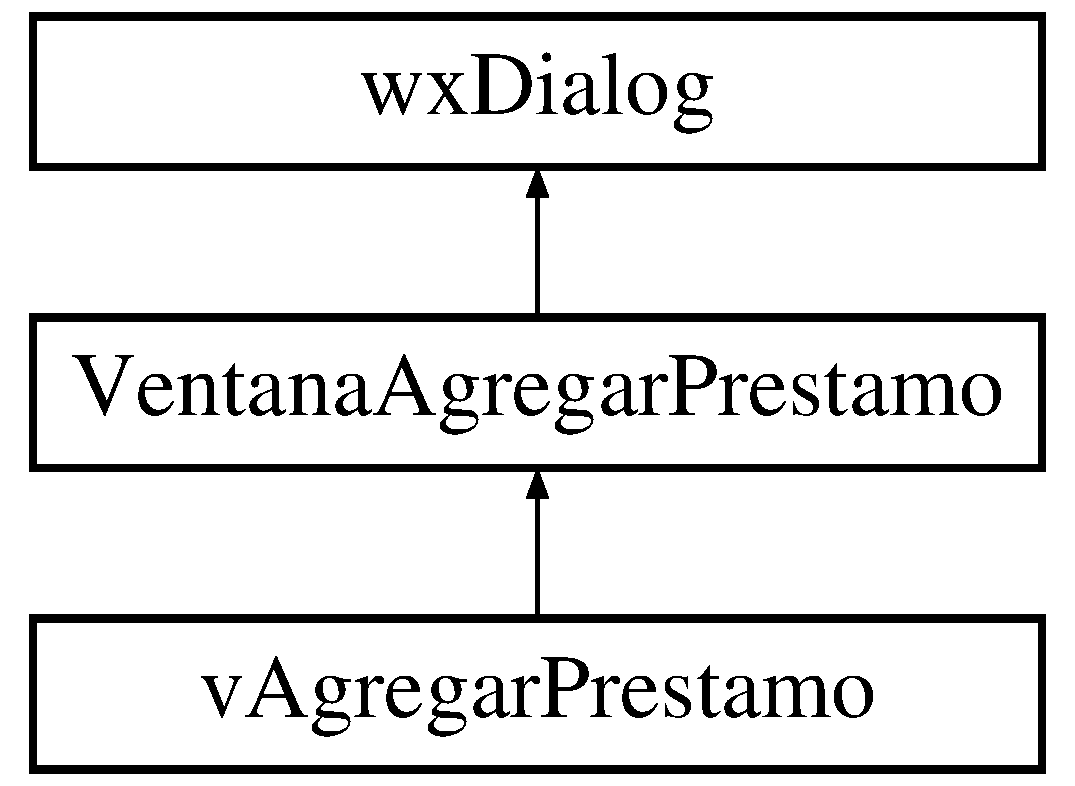
\includegraphics[height=3.000000cm]{class_ventana_agregar_prestamo}
\end{center}
\end{figure}
\subsection*{Public Member Functions}
\begin{DoxyCompactItemize}
\item 
{\bfseries Ventana\+Agregar\+Prestamo} (wx\+Window $\ast$parent, wx\+Window\+ID id=wx\+I\+D\+\_\+\+A\+NY, const wx\+String \&title=wxT(\char`\"{}Agregar Pr�stamo\char`\"{}), const wx\+Point \&pos=wx\+Default\+Position, const wx\+Size \&size=wx\+Size(470, 153), long style=wx\+D\+E\+F\+A\+U\+L\+T\+\_\+\+D\+I\+A\+L\+O\+G\+\_\+\+S\+T\+Y\+LE)\hypertarget{class_ventana_agregar_prestamo_a70373cbc49be1eae167f996677691ebb}{}\label{class_ventana_agregar_prestamo_a70373cbc49be1eae167f996677691ebb}

\end{DoxyCompactItemize}
\subsection*{Protected Member Functions}
\begin{DoxyCompactItemize}
\item 
virtual void {\bfseries Click\+Buscar\+Libro} (wx\+Command\+Event \&event)\hypertarget{class_ventana_agregar_prestamo_a11ebf3f723fd0e81135be3cb024d01f6}{}\label{class_ventana_agregar_prestamo_a11ebf3f723fd0e81135be3cb024d01f6}

\item 
virtual void {\bfseries Click\+Buscar\+Lector} (wx\+Command\+Event \&event)\hypertarget{class_ventana_agregar_prestamo_a5fefe8ca039f3eb9826a66b436fc22ed}{}\label{class_ventana_agregar_prestamo_a5fefe8ca039f3eb9826a66b436fc22ed}

\item 
virtual void {\bfseries Click\+Cancelar} (wx\+Command\+Event \&event)\hypertarget{class_ventana_agregar_prestamo_a682feebe534f74afb9689f1458f99eb6}{}\label{class_ventana_agregar_prestamo_a682feebe534f74afb9689f1458f99eb6}

\item 
virtual void {\bfseries Click\+Aceptar\+Prestamo} (wx\+Command\+Event \&event)\hypertarget{class_ventana_agregar_prestamo_a2b05031e914e671cea637e49b0d07cb8}{}\label{class_ventana_agregar_prestamo_a2b05031e914e671cea637e49b0d07cb8}

\end{DoxyCompactItemize}
\subsection*{Protected Attributes}
\begin{DoxyCompactItemize}
\item 
wx\+Static\+Text $\ast$ {\bfseries m\+\_\+static\+Text39}\hypertarget{class_ventana_agregar_prestamo_a63fbb74dee3e4c831c6dd33b391ef214}{}\label{class_ventana_agregar_prestamo_a63fbb74dee3e4c831c6dd33b391ef214}

\item 
wx\+Static\+Text $\ast$ {\bfseries l\+Libro}\hypertarget{class_ventana_agregar_prestamo_a7d41d2b735b427cd4129382b74d997f0}{}\label{class_ventana_agregar_prestamo_a7d41d2b735b427cd4129382b74d997f0}

\item 
wx\+Button $\ast$ {\bfseries b\+Buscar\+Libro}\hypertarget{class_ventana_agregar_prestamo_a478cf3e42146cf4e4eb9bfe939cc350c}{}\label{class_ventana_agregar_prestamo_a478cf3e42146cf4e4eb9bfe939cc350c}

\item 
wx\+Static\+Text $\ast$ {\bfseries m\+\_\+static\+Text391}\hypertarget{class_ventana_agregar_prestamo_af87538ced979d1477a72a02d7e463c11}{}\label{class_ventana_agregar_prestamo_af87538ced979d1477a72a02d7e463c11}

\item 
wx\+Static\+Text $\ast$ {\bfseries l\+Lector}\hypertarget{class_ventana_agregar_prestamo_a44f2a46ce5d942c91b35a76c70f75a7d}{}\label{class_ventana_agregar_prestamo_a44f2a46ce5d942c91b35a76c70f75a7d}

\item 
wx\+Button $\ast$ {\bfseries b\+Buscar\+Lector}\hypertarget{class_ventana_agregar_prestamo_a1855223342430f8ca12186ffc8513df1}{}\label{class_ventana_agregar_prestamo_a1855223342430f8ca12186ffc8513df1}

\item 
wx\+Static\+Line $\ast$ {\bfseries m\+\_\+staticline1}\hypertarget{class_ventana_agregar_prestamo_a2850f1414306cecb3b6205790344fb09}{}\label{class_ventana_agregar_prestamo_a2850f1414306cecb3b6205790344fb09}

\item 
wx\+Button $\ast$ {\bfseries b\+Cancelar}\hypertarget{class_ventana_agregar_prestamo_a42950e43a222b2faf91a56437ed0e4ca}{}\label{class_ventana_agregar_prestamo_a42950e43a222b2faf91a56437ed0e4ca}

\item 
wx\+Button $\ast$ {\bfseries b\+Confirmar\+Prestamo}\hypertarget{class_ventana_agregar_prestamo_a784e9a3dece336d34a9965f3219454c5}{}\label{class_ventana_agregar_prestamo_a784e9a3dece336d34a9965f3219454c5}

\end{DoxyCompactItemize}


\subsection{Detailed Description}
Class \hyperlink{class_ventana_agregar_prestamo}{Ventana\+Agregar\+Prestamo}. 

The documentation for this class was generated from the following files\+:\begin{DoxyCompactItemize}
\item 
Ventanas.\+h\item 
Ventanas.\+cpp\end{DoxyCompactItemize}

\hypertarget{class_ventana_buscar_lector}{}\section{Ventana\+Buscar\+Lector Class Reference}
\label{class_ventana_buscar_lector}\index{Ventana\+Buscar\+Lector@{Ventana\+Buscar\+Lector}}


Class \hyperlink{class_ventana_buscar_lector}{Ventana\+Buscar\+Lector}.  




{\ttfamily \#include $<$Ventanas.\+h$>$}

Inheritance diagram for Ventana\+Buscar\+Lector\+:\begin{figure}[H]
\begin{center}
\leavevmode
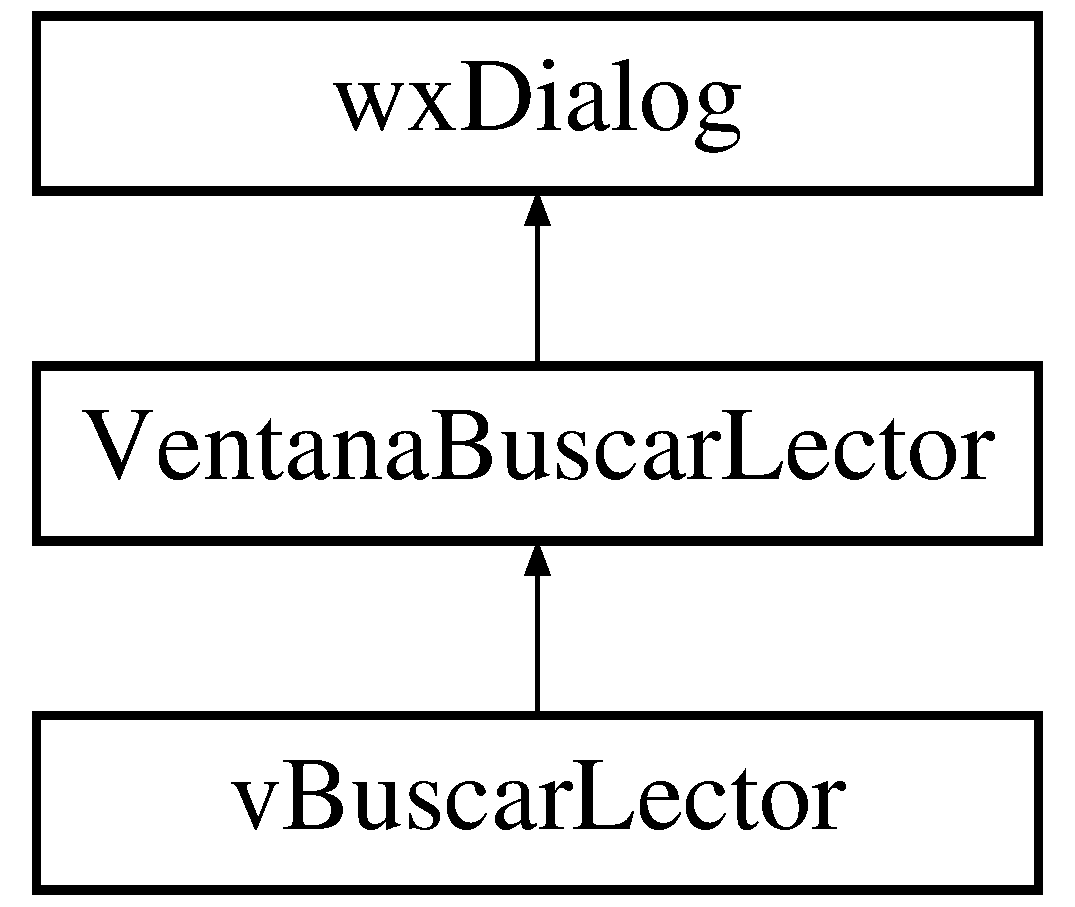
\includegraphics[height=3.000000cm]{class_ventana_buscar_lector}
\end{center}
\end{figure}
\subsection*{Public Member Functions}
\begin{DoxyCompactItemize}
\item 
{\bfseries Ventana\+Buscar\+Lector} (wx\+Window $\ast$parent, wx\+Window\+ID id=wx\+I\+D\+\_\+\+A\+NY, const wx\+String \&title=wxT(\char`\"{}Agregar Pr�stamo\char`\"{}), const wx\+Point \&pos=wx\+Default\+Position, const wx\+Size \&size=wx\+Size(904, 563), long style=wx\+D\+E\+F\+A\+U\+L\+T\+\_\+\+D\+I\+A\+L\+O\+G\+\_\+\+S\+T\+Y\+LE)\hypertarget{class_ventana_buscar_lector_a416fab5db972f4000767626ab01c980a}{}\label{class_ventana_buscar_lector_a416fab5db972f4000767626ab01c980a}

\end{DoxyCompactItemize}
\subsection*{Protected Member Functions}
\begin{DoxyCompactItemize}
\item 
virtual void {\bfseries Click\+Busqueda\+Por\+Nombre} (wx\+Command\+Event \&event)\hypertarget{class_ventana_buscar_lector_a53c5e8d4f55597ee8de39de803b86f3e}{}\label{class_ventana_buscar_lector_a53c5e8d4f55597ee8de39de803b86f3e}

\item 
virtual void {\bfseries D\+Click\+Aceptar\+Lector\+Prestamo} (wx\+Grid\+Event \&event)\hypertarget{class_ventana_buscar_lector_a3364e44650a2601b9df1b1a58616396e}{}\label{class_ventana_buscar_lector_a3364e44650a2601b9df1b1a58616396e}

\end{DoxyCompactItemize}
\subsection*{Protected Attributes}
\begin{DoxyCompactItemize}
\item 
wx\+Static\+Text $\ast$ {\bfseries m\+\_\+static\+Text2}\hypertarget{class_ventana_buscar_lector_a666779e715f4bbb178c0b77775066e9e}{}\label{class_ventana_buscar_lector_a666779e715f4bbb178c0b77775066e9e}

\item 
wx\+Text\+Ctrl $\ast$ {\bfseries t\+Busqueda\+Nombre}\hypertarget{class_ventana_buscar_lector_a5b7b2a2e1e661c7dc711e3b678147b80}{}\label{class_ventana_buscar_lector_a5b7b2a2e1e661c7dc711e3b678147b80}

\item 
wx\+Button $\ast$ {\bfseries b\+Busqueda\+Nombre}\hypertarget{class_ventana_buscar_lector_ad276e60202cc3dc20294a9783e240c63}{}\label{class_ventana_buscar_lector_ad276e60202cc3dc20294a9783e240c63}

\item 
wx\+Panel $\ast$ {\bfseries p\+Grilla\+Lectores}\hypertarget{class_ventana_buscar_lector_ab590b111ed40e60b5d0a94eed63f22a1}{}\label{class_ventana_buscar_lector_ab590b111ed40e60b5d0a94eed63f22a1}

\item 
wx\+Grid $\ast$ {\bfseries g\+Lectores\+Prestamo}\hypertarget{class_ventana_buscar_lector_affa75c05399f00c418db1a3476bc4fbc}{}\label{class_ventana_buscar_lector_affa75c05399f00c418db1a3476bc4fbc}

\end{DoxyCompactItemize}


\subsection{Detailed Description}
Class \hyperlink{class_ventana_buscar_lector}{Ventana\+Buscar\+Lector}. 

The documentation for this class was generated from the following files\+:\begin{DoxyCompactItemize}
\item 
Ventanas.\+h\item 
Ventanas.\+cpp\end{DoxyCompactItemize}

\hypertarget{class_ventana_buscar_libro}{}\section{Ventana\+Buscar\+Libro Class Reference}
\label{class_ventana_buscar_libro}\index{Ventana\+Buscar\+Libro@{Ventana\+Buscar\+Libro}}


Class \hyperlink{class_ventana_buscar_libro}{Ventana\+Buscar\+Libro}.  




{\ttfamily \#include $<$Ventanas.\+h$>$}

Inheritance diagram for Ventana\+Buscar\+Libro\+:\begin{figure}[H]
\begin{center}
\leavevmode
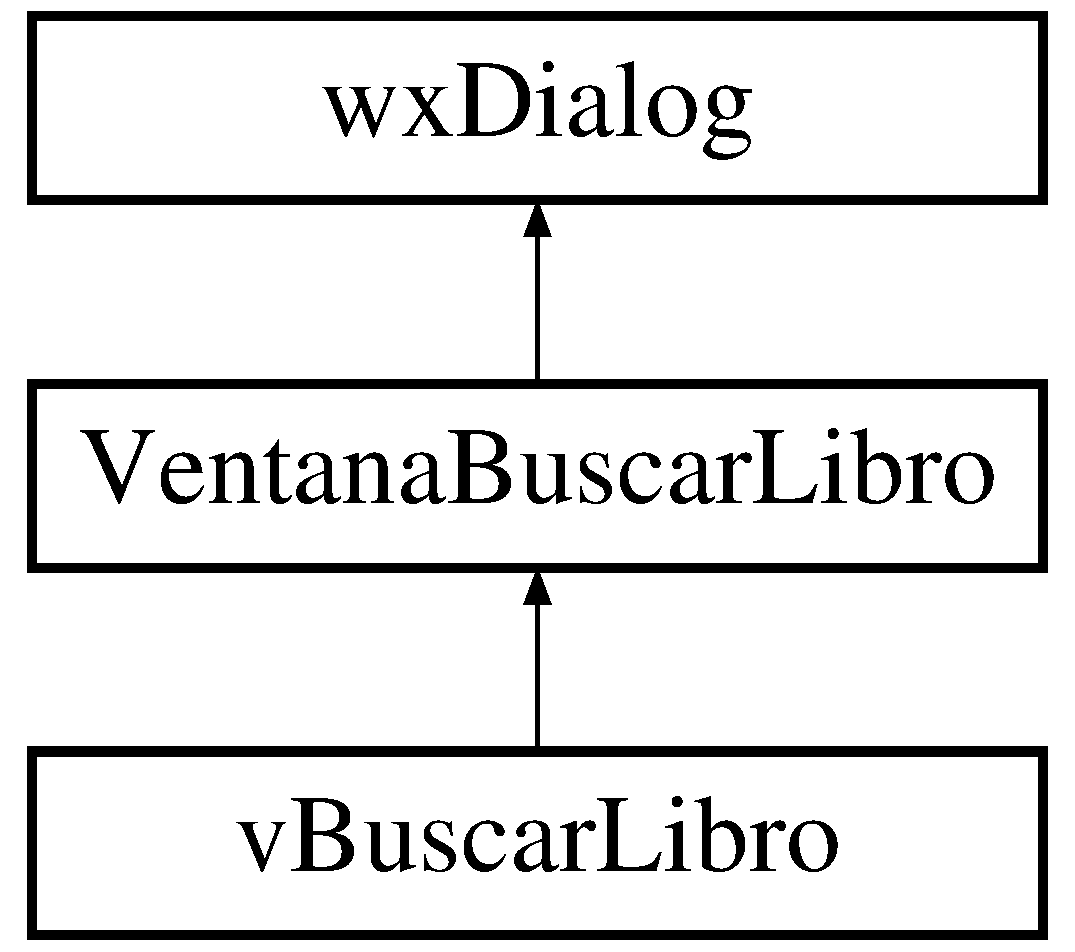
\includegraphics[height=3.000000cm]{class_ventana_buscar_libro}
\end{center}
\end{figure}
\subsection*{Public Member Functions}
\begin{DoxyCompactItemize}
\item 
{\bfseries Ventana\+Buscar\+Libro} (wx\+Window $\ast$parent, wx\+Window\+ID id=wx\+I\+D\+\_\+\+A\+NY, const wx\+String \&title=wxT(\char`\"{}Agregar Pr�stamo\char`\"{}), const wx\+Point \&pos=wx\+Default\+Position, const wx\+Size \&size=wx\+Size(904, 563), long style=wx\+D\+E\+F\+A\+U\+L\+T\+\_\+\+D\+I\+A\+L\+O\+G\+\_\+\+S\+T\+Y\+LE)\hypertarget{class_ventana_buscar_libro_a8037003902da52388fc43a4c0773a924}{}\label{class_ventana_buscar_libro_a8037003902da52388fc43a4c0773a924}

\end{DoxyCompactItemize}
\subsection*{Protected Member Functions}
\begin{DoxyCompactItemize}
\item 
virtual void {\bfseries Click\+Busqueda\+Por\+Titulo} (wx\+Command\+Event \&event)\hypertarget{class_ventana_buscar_libro_aa2a2199164472385ba14ae7a6cc4fbb7}{}\label{class_ventana_buscar_libro_aa2a2199164472385ba14ae7a6cc4fbb7}

\item 
virtual void {\bfseries D\+Click\+Aceptar\+Libro\+Prestamo} (wx\+Grid\+Event \&event)\hypertarget{class_ventana_buscar_libro_ae1516e482a4f8e922c95a396c6c3b5bc}{}\label{class_ventana_buscar_libro_ae1516e482a4f8e922c95a396c6c3b5bc}

\end{DoxyCompactItemize}
\subsection*{Protected Attributes}
\begin{DoxyCompactItemize}
\item 
wx\+Static\+Text $\ast$ {\bfseries m\+\_\+static\+Text2}\hypertarget{class_ventana_buscar_libro_a2643f888fa08b1cbb0359383fb9317d0}{}\label{class_ventana_buscar_libro_a2643f888fa08b1cbb0359383fb9317d0}

\item 
wx\+Text\+Ctrl $\ast$ {\bfseries t\+Busqueda\+Titulo}\hypertarget{class_ventana_buscar_libro_a2ffb9e6e248740526e2447cca0ce76e4}{}\label{class_ventana_buscar_libro_a2ffb9e6e248740526e2447cca0ce76e4}

\item 
wx\+Button $\ast$ {\bfseries b\+Busqueda\+Titulo}\hypertarget{class_ventana_buscar_libro_ae192e8389cd2fef0329a6f39ab0959f3}{}\label{class_ventana_buscar_libro_ae192e8389cd2fef0329a6f39ab0959f3}

\item 
wx\+Panel $\ast$ {\bfseries p\+Grilla\+Libros}\hypertarget{class_ventana_buscar_libro_aef903c113af8a3dece33de3dd8cc9340}{}\label{class_ventana_buscar_libro_aef903c113af8a3dece33de3dd8cc9340}

\item 
wx\+Grid $\ast$ {\bfseries g\+Libros\+Prestamo}\hypertarget{class_ventana_buscar_libro_a1487c3bc8feb92d4090262c3f2dc044e}{}\label{class_ventana_buscar_libro_a1487c3bc8feb92d4090262c3f2dc044e}

\end{DoxyCompactItemize}


\subsection{Detailed Description}
Class \hyperlink{class_ventana_buscar_libro}{Ventana\+Buscar\+Libro}. 

The documentation for this class was generated from the following files\+:\begin{DoxyCompactItemize}
\item 
Ventanas.\+h\item 
Ventanas.\+cpp\end{DoxyCompactItemize}

\hypertarget{class_ventana_principal}{}\section{Ventana\+Principal Class Reference}
\label{class_ventana_principal}\index{Ventana\+Principal@{Ventana\+Principal}}


Class \hyperlink{class_ventana_principal}{Ventana\+Principal}.  




{\ttfamily \#include $<$Ventanas.\+h$>$}

Inheritance diagram for Ventana\+Principal\+:\begin{figure}[H]
\begin{center}
\leavevmode
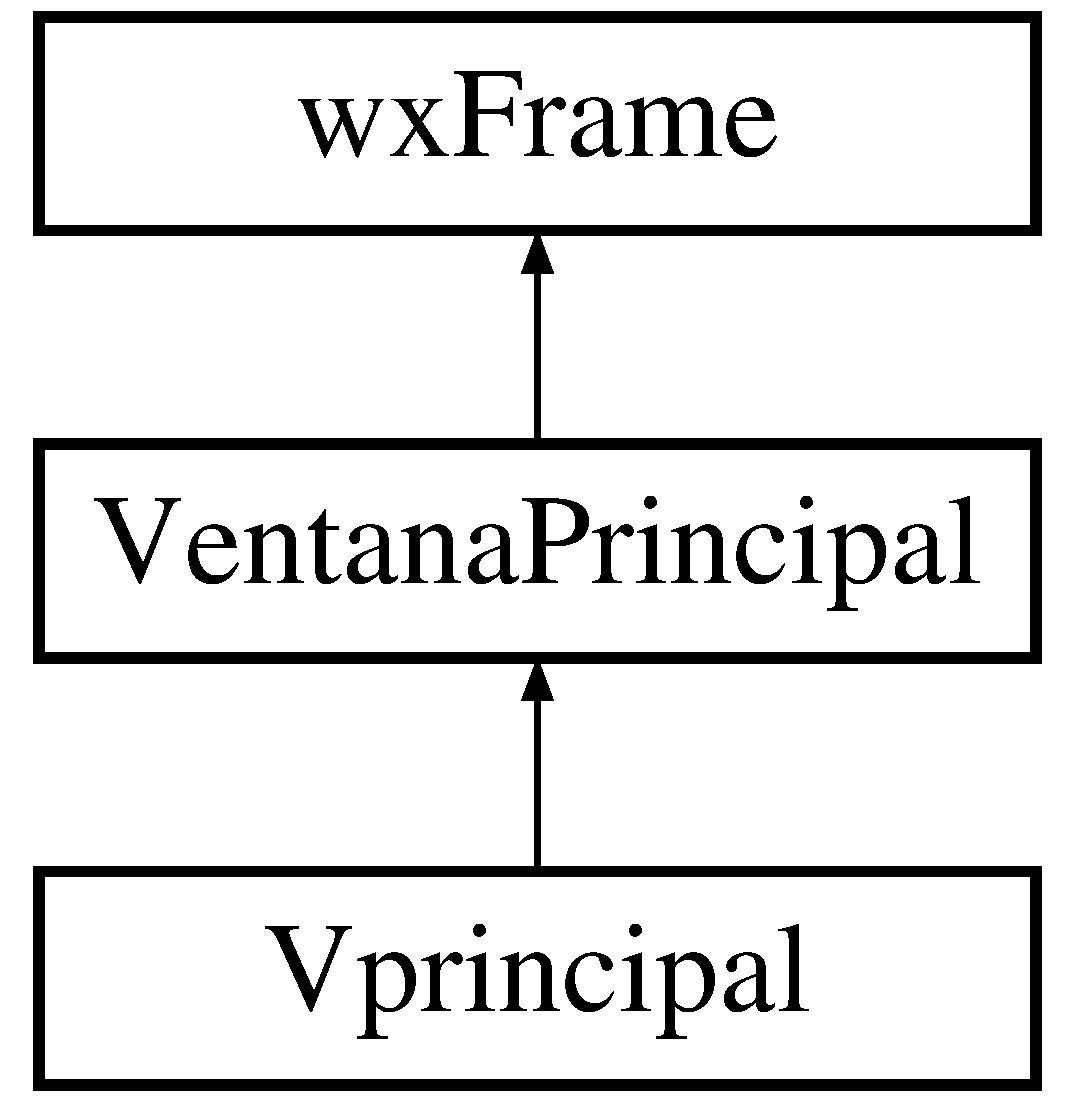
\includegraphics[height=3.000000cm]{class_ventana_principal}
\end{center}
\end{figure}
\subsection*{Public Member Functions}
\begin{DoxyCompactItemize}
\item 
{\bfseries Ventana\+Principal} (wx\+Window $\ast$parent, wx\+Window\+ID id=wx\+I\+D\+\_\+\+A\+NY, const wx\+String \&title=wxT(\char`\"{}Corinthian\char`\"{}), const wx\+Point \&pos=wx\+Default\+Position, const wx\+Size \&size=wx\+Size(829, 600), long style=wx\+D\+E\+F\+A\+U\+L\+T\+\_\+\+F\+R\+A\+M\+E\+\_\+\+S\+T\+Y\+LE$\vert$wx\+T\+A\+B\+\_\+\+T\+R\+A\+V\+E\+R\+S\+AL)\hypertarget{class_ventana_principal_a92ee5cfcc9fda6049f70d28d5b30065b}{}\label{class_ventana_principal_a92ee5cfcc9fda6049f70d28d5b30065b}

\end{DoxyCompactItemize}
\subsection*{Protected Member Functions}
\begin{DoxyCompactItemize}
\item 
virtual void {\bfseries Click\+Agregar\+Libro\+Menu} (wx\+Command\+Event \&event)\hypertarget{class_ventana_principal_a8516dfa50e0a94078dc1d08fecbaab99}{}\label{class_ventana_principal_a8516dfa50e0a94078dc1d08fecbaab99}

\item 
virtual void {\bfseries Click\+Agregar\+Lector\+Menu} (wx\+Command\+Event \&event)\hypertarget{class_ventana_principal_a562996206a804852b54b3a4bcdc99755}{}\label{class_ventana_principal_a562996206a804852b54b3a4bcdc99755}

\item 
virtual void {\bfseries Click\+Pestania\+Libros} (wx\+Mouse\+Event \&event)\hypertarget{class_ventana_principal_ada4bd8adede2869bfc8c13a2f0e8afa3}{}\label{class_ventana_principal_ada4bd8adede2869bfc8c13a2f0e8afa3}

\item 
virtual void {\bfseries Click\+Derecho\+Grilla\+Libro} (wx\+Grid\+Event \&event)\hypertarget{class_ventana_principal_aca11c056b12f20b0908f9274523fd036}{}\label{class_ventana_principal_aca11c056b12f20b0908f9274523fd036}

\item 
virtual void {\bfseries Click\+Busqueda\+Por\+Titulo} (wx\+Command\+Event \&event)\hypertarget{class_ventana_principal_a96b52de26d860861d06aa264c95de97d}{}\label{class_ventana_principal_a96b52de26d860861d06aa264c95de97d}

\item 
virtual void {\bfseries Click\+Pestania\+Lectores} (wx\+Mouse\+Event \&event)\hypertarget{class_ventana_principal_aaad9dd7b93f35d7aef9a5db4e8dc0c3e}{}\label{class_ventana_principal_aaad9dd7b93f35d7aef9a5db4e8dc0c3e}

\item 
virtual void {\bfseries Click\+Derecho\+Grilla\+Lectores} (wx\+Grid\+Event \&event)\hypertarget{class_ventana_principal_a45ff4b8276750dd6277f556e0241ad19}{}\label{class_ventana_principal_a45ff4b8276750dd6277f556e0241ad19}

\item 
virtual void {\bfseries Click\+Busqueda\+Por\+Nombre} (wx\+Command\+Event \&event)\hypertarget{class_ventana_principal_a947b45816c4647162a4b6cad3b0d53d9}{}\label{class_ventana_principal_a947b45816c4647162a4b6cad3b0d53d9}

\item 
virtual void {\bfseries Click\+Pestania\+Prestamos} (wx\+Mouse\+Event \&event)\hypertarget{class_ventana_principal_ac0833257e62cfac7d74a95450f45e7a0}{}\label{class_ventana_principal_ac0833257e62cfac7d74a95450f45e7a0}

\item 
virtual void {\bfseries Click\+Derecho\+Grilla\+Prestamo} (wx\+Grid\+Event \&event)\hypertarget{class_ventana_principal_a8f32970e70d10ba4c73a70b8bb5f8bbb}{}\label{class_ventana_principal_a8f32970e70d10ba4c73a70b8bb5f8bbb}

\item 
virtual void {\bfseries Click\+Busqueda\+Prestamo} (wx\+Command\+Event \&event)\hypertarget{class_ventana_principal_afd74ce768966f8b29797a7c25bc32ca9}{}\label{class_ventana_principal_afd74ce768966f8b29797a7c25bc32ca9}

\item 
virtual void {\bfseries Click\+Pestania\+Sanciones} (wx\+Mouse\+Event \&event)\hypertarget{class_ventana_principal_a54555224258636f89fd277cd83952975}{}\label{class_ventana_principal_a54555224258636f89fd277cd83952975}

\end{DoxyCompactItemize}
\subsection*{Protected Attributes}
\begin{DoxyCompactItemize}
\item 
wx\+Menu\+Bar $\ast$ {\bfseries m\+\_\+menubar2}\hypertarget{class_ventana_principal_a037872398aa7f834dc848f1930898aa2}{}\label{class_ventana_principal_a037872398aa7f834dc848f1930898aa2}

\item 
wx\+Menu $\ast$ {\bfseries m\+\_\+menu2}\hypertarget{class_ventana_principal_a2db591eb628e107c8e1541339abeaed5}{}\label{class_ventana_principal_a2db591eb628e107c8e1541339abeaed5}

\item 
wx\+Notebook $\ast$ {\bfseries m\+\_\+notebook2}\hypertarget{class_ventana_principal_a3aefd421c4cc41d5d0a053aad662e39d}{}\label{class_ventana_principal_a3aefd421c4cc41d5d0a053aad662e39d}

\item 
wx\+Panel $\ast$ {\bfseries p\+Grilla\+Libros}\hypertarget{class_ventana_principal_a2ea6c64bb5a057881d846ef63162f3e6}{}\label{class_ventana_principal_a2ea6c64bb5a057881d846ef63162f3e6}

\item 
wx\+Grid $\ast$ {\bfseries g\+Libros}\hypertarget{class_ventana_principal_a40d77b85c974aba85476e27e5105b96c}{}\label{class_ventana_principal_a40d77b85c974aba85476e27e5105b96c}

\item 
wx\+Static\+Text $\ast$ {\bfseries m\+\_\+static\+Text2}\hypertarget{class_ventana_principal_ab241c6977c05dcdea78d8dc315a6872e}{}\label{class_ventana_principal_ab241c6977c05dcdea78d8dc315a6872e}

\item 
wx\+Text\+Ctrl $\ast$ {\bfseries t\+Busqueda\+Titulo}\hypertarget{class_ventana_principal_ae3990db3e5da1ccfac3677a418c1f1f6}{}\label{class_ventana_principal_ae3990db3e5da1ccfac3677a418c1f1f6}

\item 
wx\+Button $\ast$ {\bfseries b\+Busqueda\+Titulo}\hypertarget{class_ventana_principal_a80ad50bc1fe24e5bf042365df5978756}{}\label{class_ventana_principal_a80ad50bc1fe24e5bf042365df5978756}

\item 
wx\+Panel $\ast$ {\bfseries p\+Grilla\+Lectores}\hypertarget{class_ventana_principal_a065f6cc568ad3ffededaeb8bdf312a88}{}\label{class_ventana_principal_a065f6cc568ad3ffededaeb8bdf312a88}

\item 
wx\+Grid $\ast$ {\bfseries g\+Lectores}\hypertarget{class_ventana_principal_a261eb27263a3d1d1c16fdbf30309f3c4}{}\label{class_ventana_principal_a261eb27263a3d1d1c16fdbf30309f3c4}

\item 
wx\+Static\+Text $\ast$ {\bfseries m\+\_\+static\+Text21}\hypertarget{class_ventana_principal_ae133a580170066e8eb97f0c35de9f079}{}\label{class_ventana_principal_ae133a580170066e8eb97f0c35de9f079}

\item 
wx\+Text\+Ctrl $\ast$ {\bfseries t\+Busqueda\+Nombre}\hypertarget{class_ventana_principal_ac9e9018e6bcdb5312e21645070f5ea14}{}\label{class_ventana_principal_ac9e9018e6bcdb5312e21645070f5ea14}

\item 
wx\+Button $\ast$ {\bfseries b\+Busqueda\+Nombre}\hypertarget{class_ventana_principal_a9c5e23d6b7332497c4953e9e98eaa99f}{}\label{class_ventana_principal_a9c5e23d6b7332497c4953e9e98eaa99f}

\item 
wx\+Panel $\ast$ {\bfseries p\+Grilla\+Prestamos}\hypertarget{class_ventana_principal_a5872db5495f47e4db328c14fcdaf926d}{}\label{class_ventana_principal_a5872db5495f47e4db328c14fcdaf926d}

\item 
wx\+Grid $\ast$ {\bfseries g\+Prestamos}\hypertarget{class_ventana_principal_ac0e323ab4fd44b9318bfdf0dd4151090}{}\label{class_ventana_principal_ac0e323ab4fd44b9318bfdf0dd4151090}

\item 
wx\+Static\+Text $\ast$ {\bfseries m\+\_\+static\+Text22}\hypertarget{class_ventana_principal_a70b8fef655d3fbe81cbbed259a38a9d8}{}\label{class_ventana_principal_a70b8fef655d3fbe81cbbed259a38a9d8}

\item 
wx\+Text\+Ctrl $\ast$ {\bfseries t\+Busqueda\+Prestamo}\hypertarget{class_ventana_principal_a9b94a53c0c8d888df6f5fb8c2c2e13de}{}\label{class_ventana_principal_a9b94a53c0c8d888df6f5fb8c2c2e13de}

\item 
wx\+Button $\ast$ {\bfseries b\+Busqueda\+Prestamo}\hypertarget{class_ventana_principal_af48cf4a54a346da26308604758d948dd}{}\label{class_ventana_principal_af48cf4a54a346da26308604758d948dd}

\item 
wx\+Panel $\ast$ {\bfseries p\+Grilla\+Sanciones}\hypertarget{class_ventana_principal_a5f7605f2ec2b8e41510e989546064fed}{}\label{class_ventana_principal_a5f7605f2ec2b8e41510e989546064fed}

\item 
wx\+Grid $\ast$ {\bfseries g\+Sanciones}\hypertarget{class_ventana_principal_ad749ae06e20c4a62ee4a9ebaba6fbdf4}{}\label{class_ventana_principal_ad749ae06e20c4a62ee4a9ebaba6fbdf4}

\end{DoxyCompactItemize}


\subsection{Detailed Description}
Class \hyperlink{class_ventana_principal}{Ventana\+Principal}. 

The documentation for this class was generated from the following files\+:\begin{DoxyCompactItemize}
\item 
Ventanas.\+h\item 
Ventanas.\+cpp\end{DoxyCompactItemize}

\hypertarget{classv_modificar_lector}{}\section{v\+Modificar\+Lector Class Reference}
\label{classv_modificar_lector}\index{v\+Modificar\+Lector@{v\+Modificar\+Lector}}


Ventana para modificar los datos de un lector.  




{\ttfamily \#include $<$v\+Modificar\+Lector.\+h$>$}

Inheritance diagram for v\+Modificar\+Lector\+:\begin{figure}[H]
\begin{center}
\leavevmode
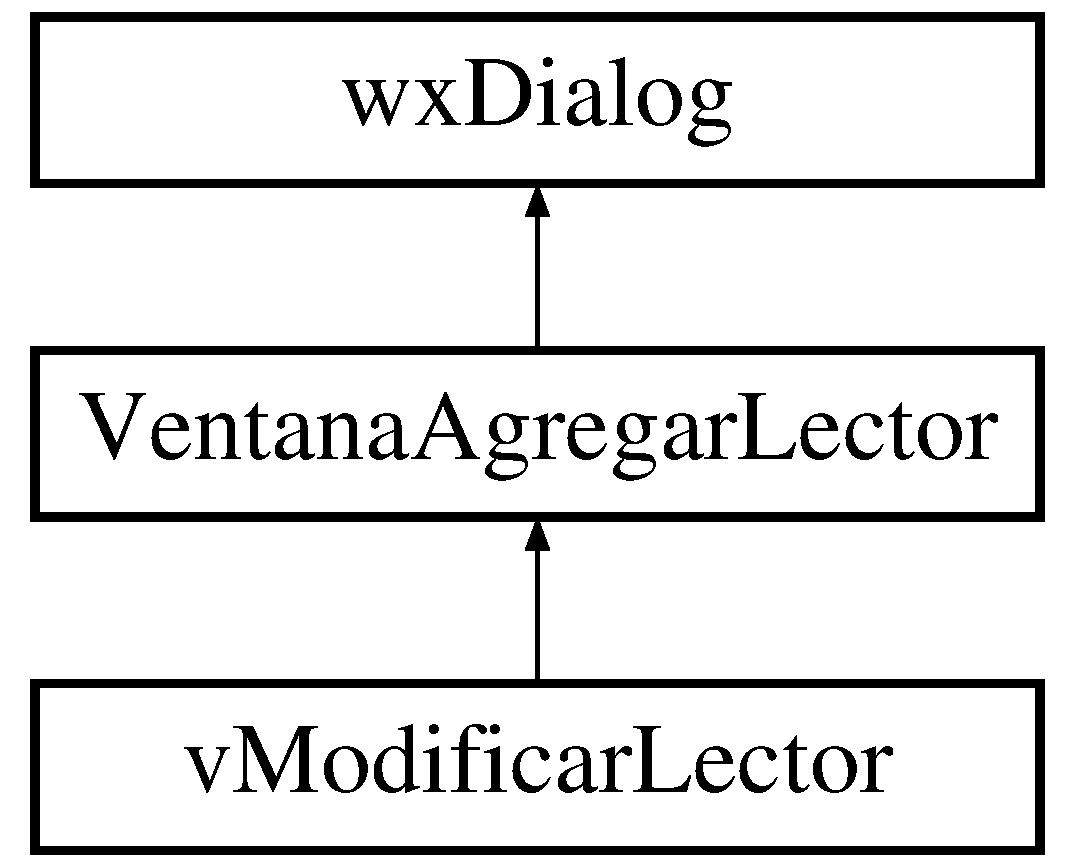
\includegraphics[height=3.000000cm]{classv_modificar_lector}
\end{center}
\end{figure}
\subsection*{Public Member Functions}
\begin{DoxyCompactItemize}
\item 
{\bfseries v\+Modificar\+Lector} (wx\+Window $\ast$parent=N\+U\+LL)\hypertarget{classv_modificar_lector_a81540c53d35a0fcb70b7c6823a0fa4fc}{}\label{classv_modificar_lector_a81540c53d35a0fcb70b7c6823a0fa4fc}

\item 
string \hyperlink{classv_modificar_lector_a3877690ffa6dbf03576d430229d4b43e}{Validar\+Datos} ()\hypertarget{classv_modificar_lector_a3877690ffa6dbf03576d430229d4b43e}{}\label{classv_modificar_lector_a3877690ffa6dbf03576d430229d4b43e}

\begin{DoxyCompactList}\small\item\em Valida los datos ingresados. \end{DoxyCompactList}\end{DoxyCompactItemize}
\subsection*{Static Public Attributes}
\begin{DoxyCompactItemize}
\item 
static int \hyperlink{classv_modificar_lector_a8689006bf9267260d9207ddcc11eb164}{num\+Lector} = -\/1
\begin{DoxyCompactList}\small\item\em variable estatica del n�mero del lector \end{DoxyCompactList}\end{DoxyCompactItemize}
\subsection*{Protected Member Functions}
\begin{DoxyCompactItemize}
\item 
void \hyperlink{classv_modificar_lector_ae4607c781efe7577df431c9c888527a7}{b\+Cancelar\+Agregar\+Lector} (wx\+Command\+Event \&event)\hypertarget{classv_modificar_lector_ae4607c781efe7577df431c9c888527a7}{}\label{classv_modificar_lector_ae4607c781efe7577df431c9c888527a7}

\begin{DoxyCompactList}\small\item\em Cierra la ventana sin modificar (boton \char`\"{}\+Cancelar\char`\"{}) \end{DoxyCompactList}\item 
void \hyperlink{classv_modificar_lector_a858e4bbe78e0a3fd6aeafb0bbf9e1971}{Click\+Agregar\+Lector\+Nuevo} (wx\+Command\+Event \&event)\hypertarget{classv_modificar_lector_a858e4bbe78e0a3fd6aeafb0bbf9e1971}{}\label{classv_modificar_lector_a858e4bbe78e0a3fd6aeafb0bbf9e1971}

\begin{DoxyCompactList}\small\item\em Cierra la ventana modificando los datos (boton \char`\"{}\+Cancelar\char`\"{}) \end{DoxyCompactList}\end{DoxyCompactItemize}
\subsection*{Additional Inherited Members}


\subsection{Detailed Description}
Ventana para modificar los datos de un lector. 

\subsection{Member Data Documentation}
\index{v\+Modificar\+Lector@{v\+Modificar\+Lector}!num\+Lector@{num\+Lector}}
\index{num\+Lector@{num\+Lector}!v\+Modificar\+Lector@{v\+Modificar\+Lector}}
\subsubsection[{\texorpdfstring{num\+Lector}{numLector}}]{\setlength{\rightskip}{0pt plus 5cm}int v\+Modificar\+Lector\+::num\+Lector = -\/1\hspace{0.3cm}{\ttfamily [static]}}\hypertarget{classv_modificar_lector_a8689006bf9267260d9207ddcc11eb164}{}\label{classv_modificar_lector_a8689006bf9267260d9207ddcc11eb164}


variable estatica del n�mero del lector 

Implementa los metodos para modificar los datos de un lector. 

The documentation for this class was generated from the following files\+:\begin{DoxyCompactItemize}
\item 
v\+Modificar\+Lector.\+h\item 
v\+Modificar\+Lector.\+cpp\end{DoxyCompactItemize}

\hypertarget{classv_modificar_libro}{}\section{v\+Modificar\+Libro Class Reference}
\label{classv_modificar_libro}\index{v\+Modificar\+Libro@{v\+Modificar\+Libro}}


Ventana para modificar los datos de un libro.  




{\ttfamily \#include $<$v\+Modificar\+Libro.\+h$>$}

Inheritance diagram for v\+Modificar\+Libro\+:\begin{figure}[H]
\begin{center}
\leavevmode
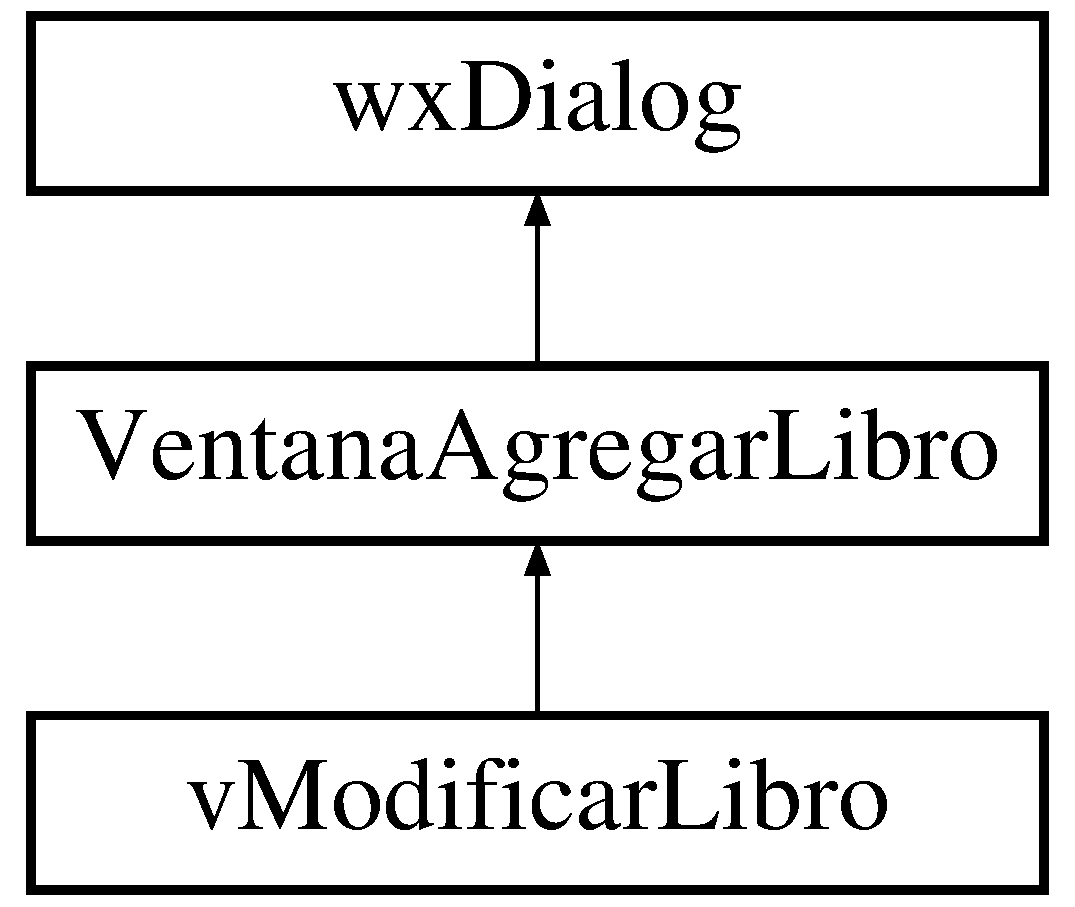
\includegraphics[height=3.000000cm]{classv_modificar_libro}
\end{center}
\end{figure}
\subsection*{Public Member Functions}
\begin{DoxyCompactItemize}
\item 
{\bfseries v\+Modificar\+Libro} (wx\+Window $\ast$parent=N\+U\+LL)\hypertarget{classv_modificar_libro_ab9f38d4cbc620858c99c91dad0af5493}{}\label{classv_modificar_libro_ab9f38d4cbc620858c99c91dad0af5493}

\item 
string \hyperlink{classv_modificar_libro_a175daf636185fd7814692fed543fda21}{Validar\+Datos} ()\hypertarget{classv_modificar_libro_a175daf636185fd7814692fed543fda21}{}\label{classv_modificar_libro_a175daf636185fd7814692fed543fda21}

\begin{DoxyCompactList}\small\item\em Valida los datos ingresados. \end{DoxyCompactList}\end{DoxyCompactItemize}
\subsection*{Static Public Attributes}
\begin{DoxyCompactItemize}
\item 
static int \hyperlink{classv_modificar_libro_a88a10764b43adc0d365871ad2da42d28}{cod\+Libro} = -\/1
\begin{DoxyCompactList}\small\item\em variable estatica del codigo de libro \end{DoxyCompactList}\end{DoxyCompactItemize}
\subsection*{Protected Member Functions}
\begin{DoxyCompactItemize}
\item 
void \hyperlink{classv_modificar_libro_a3180210031e47053fb7095eb7187c36c}{b\+Cancelar\+Agregar\+Libro} (wx\+Command\+Event \&event)\hypertarget{classv_modificar_libro_a3180210031e47053fb7095eb7187c36c}{}\label{classv_modificar_libro_a3180210031e47053fb7095eb7187c36c}

\begin{DoxyCompactList}\small\item\em Cierra la ventana sin modificar (boton \char`\"{}\+Cancelar\char`\"{}) \end{DoxyCompactList}\item 
void \hyperlink{classv_modificar_libro_a45e6d79ccf09a1804dd8f0eeb7deb88d}{Click\+Agregar\+Libro\+Nuevo} (wx\+Command\+Event \&event)\hypertarget{classv_modificar_libro_a45e6d79ccf09a1804dd8f0eeb7deb88d}{}\label{classv_modificar_libro_a45e6d79ccf09a1804dd8f0eeb7deb88d}

\begin{DoxyCompactList}\small\item\em Cierra la ventana modificando los datos (boton \char`\"{}\+Cancelar\char`\"{}) \end{DoxyCompactList}\end{DoxyCompactItemize}
\subsection*{Additional Inherited Members}


\subsection{Detailed Description}
Ventana para modificar los datos de un libro. 

\subsection{Member Data Documentation}
\index{v\+Modificar\+Libro@{v\+Modificar\+Libro}!cod\+Libro@{cod\+Libro}}
\index{cod\+Libro@{cod\+Libro}!v\+Modificar\+Libro@{v\+Modificar\+Libro}}
\subsubsection[{\texorpdfstring{cod\+Libro}{codLibro}}]{\setlength{\rightskip}{0pt plus 5cm}int v\+Modificar\+Libro\+::cod\+Libro = -\/1\hspace{0.3cm}{\ttfamily [static]}}\hypertarget{classv_modificar_libro_a88a10764b43adc0d365871ad2da42d28}{}\label{classv_modificar_libro_a88a10764b43adc0d365871ad2da42d28}


variable estatica del codigo de libro 

Implementa los metodos para modificar los datos de un libro. 

The documentation for this class was generated from the following files\+:\begin{DoxyCompactItemize}
\item 
v\+Modificar\+Libro.\+h\item 
v\+Modificar\+Libro.\+cpp\end{DoxyCompactItemize}

\hypertarget{class_vprincipal}{}\section{Vprincipal Class Reference}
\label{class_vprincipal}\index{Vprincipal@{Vprincipal}}
Inheritance diagram for Vprincipal\+:\begin{figure}[H]
\begin{center}
\leavevmode
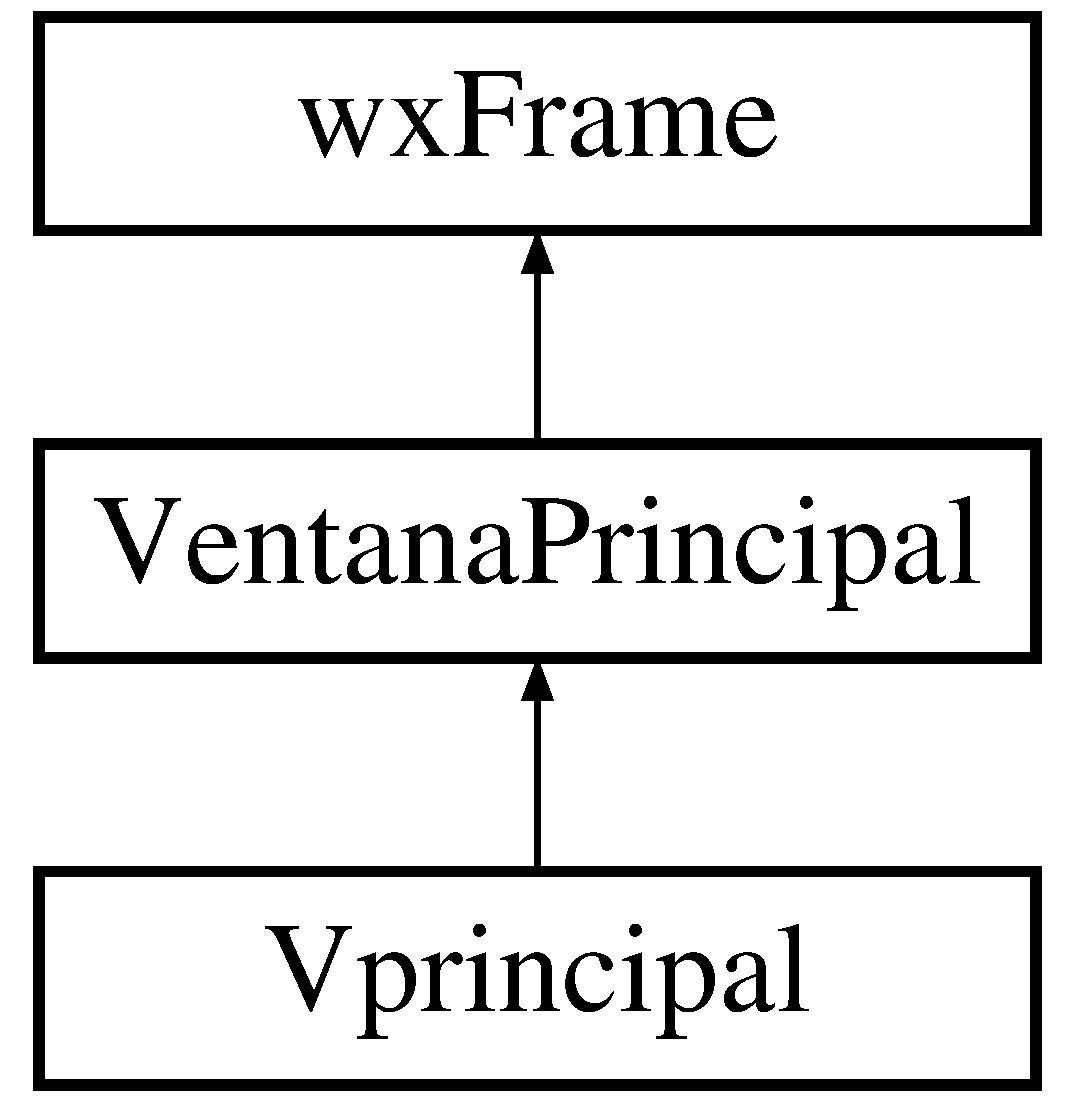
\includegraphics[height=3.000000cm]{class_vprincipal}
\end{center}
\end{figure}
\subsection*{Public Member Functions}
\begin{DoxyCompactItemize}
\item 
{\bfseries Vprincipal} (wx\+Window $\ast$parent=N\+U\+LL)\hypertarget{class_vprincipal_a278dadba79f9ca00c8407757c95c5ded}{}\label{class_vprincipal_a278dadba79f9ca00c8407757c95c5ded}

\item 
void {\bfseries Click\+Derecho\+Grilla\+Lectores} (wx\+Grid\+Event \&event)\hypertarget{class_vprincipal_a5dcf202589d06db776164b52176a084d}{}\label{class_vprincipal_a5dcf202589d06db776164b52176a084d}

\item 
void {\bfseries Click\+Derecho\+Grilla\+Libro} (wx\+Grid\+Event \&event)\hypertarget{class_vprincipal_aa27cb1c5571e1087bc5d80f9d4c579a4}{}\label{class_vprincipal_aa27cb1c5571e1087bc5d80f9d4c579a4}

\item 
void {\bfseries Click\+Derecho\+Grilla\+Prestamo} (wx\+Grid\+Event \&event)\hypertarget{class_vprincipal_a4bdbd1ad546d5e0e998c12e435a4cf5e}{}\label{class_vprincipal_a4bdbd1ad546d5e0e998c12e435a4cf5e}

\item 
void {\bfseries Popup\+Click\+Derecho\+Libro} (wx\+Command\+Event \&event)\hypertarget{class_vprincipal_a69dec2b5b12821296eb0b58bc11e6a35}{}\label{class_vprincipal_a69dec2b5b12821296eb0b58bc11e6a35}

\item 
void {\bfseries Popup\+Click\+Derecho\+Lector} (wx\+Command\+Event \&event)\hypertarget{class_vprincipal_aac7b8ff710931e75a91ae506395298af}{}\label{class_vprincipal_aac7b8ff710931e75a91ae506395298af}

\item 
void {\bfseries Popup\+Click\+Derecho\+Prestamo} (wx\+Command\+Event \&event)\hypertarget{class_vprincipal_a13b970fdbe3fcb361b946ccf91904afc}{}\label{class_vprincipal_a13b970fdbe3fcb361b946ccf91904afc}

\item 
void {\bfseries Click\+Busqueda\+Por\+Titulo} (wx\+Command\+Event \&event)\hypertarget{class_vprincipal_af929cb33fa3c5d6c3566a22a8b0de760}{}\label{class_vprincipal_af929cb33fa3c5d6c3566a22a8b0de760}

\item 
void {\bfseries Click\+Busqueda\+Por\+Nombre} (wx\+Command\+Event \&event)\hypertarget{class_vprincipal_ac2431b119c528a1395f56f426340d930}{}\label{class_vprincipal_ac2431b119c528a1395f56f426340d930}

\item 
void {\bfseries Click\+Agregar\+Sancion\+Menu} (int num\+Lector)\hypertarget{class_vprincipal_a4103b2f0ca0be4c514f3d81216df7805}{}\label{class_vprincipal_a4103b2f0ca0be4c514f3d81216df7805}

\item 
void {\bfseries Click\+Agregar\+Libro\+Menu} (wx\+Command\+Event \&event)\hypertarget{class_vprincipal_a0716d64c67c3e4c97980c6475018bf31}{}\label{class_vprincipal_a0716d64c67c3e4c97980c6475018bf31}

\item 
void {\bfseries Click\+Modificar\+Libro\+Menu} ()\hypertarget{class_vprincipal_ae8728d96a1528116d1980620651b831e}{}\label{class_vprincipal_ae8728d96a1528116d1980620651b831e}

\item 
void {\bfseries Click\+Eliminar\+Libro\+Menu} ()\hypertarget{class_vprincipal_ab2bb7ddddea0a8d31e4cb2eb355fbde6}{}\label{class_vprincipal_ab2bb7ddddea0a8d31e4cb2eb355fbde6}

\item 
void {\bfseries Click\+Agregar\+Lector\+Menu} (wx\+Command\+Event \&event)\hypertarget{class_vprincipal_a8a320e4d57369df4cf216697d9b98b55}{}\label{class_vprincipal_a8a320e4d57369df4cf216697d9b98b55}

\item 
void {\bfseries Click\+Modificar\+Lector\+Menu} ()\hypertarget{class_vprincipal_a40acdd47cfdefa0ee633ce3f1ea3a79d}{}\label{class_vprincipal_a40acdd47cfdefa0ee633ce3f1ea3a79d}

\item 
void {\bfseries Click\+Eliminar\+Lector\+Menu} ()\hypertarget{class_vprincipal_a33fced51b1e48407b6a37f3d9eb963f8}{}\label{class_vprincipal_a33fced51b1e48407b6a37f3d9eb963f8}

\item 
void {\bfseries Click\+Agregar\+Prestamo\+Menu} ()\hypertarget{class_vprincipal_a97e136123deaf0ed419202baf5d04878}{}\label{class_vprincipal_a97e136123deaf0ed419202baf5d04878}

\item 
void {\bfseries Click\+Agregar\+Devolucion\+Menu} ()\hypertarget{class_vprincipal_ae2472540ba2cfc008c7bea94e8c46da2}{}\label{class_vprincipal_ae2472540ba2cfc008c7bea94e8c46da2}

\item 
void {\bfseries Click\+Busqueda\+Prestamo} (wx\+Command\+Event \&event)\hypertarget{class_vprincipal_aeb20628f120b31509dc47937eabde165}{}\label{class_vprincipal_aeb20628f120b31509dc47937eabde165}

\item 
void {\bfseries Dibujar\+Pestania\+Libros} ()\hypertarget{class_vprincipal_afea83d672b1d6efe401fdde91c80561c}{}\label{class_vprincipal_afea83d672b1d6efe401fdde91c80561c}

\item 
void {\bfseries Dibujar\+Pestania\+Lectores} ()\hypertarget{class_vprincipal_ae3d56f1218d97426a4a4ec7ddb15259f}{}\label{class_vprincipal_ae3d56f1218d97426a4a4ec7ddb15259f}

\item 
void {\bfseries Dibujar\+Pestania\+Prestamos} ()\hypertarget{class_vprincipal_aa3c9e704305bc2b949ba1f647af9ffd7}{}\label{class_vprincipal_aa3c9e704305bc2b949ba1f647af9ffd7}

\item 
void {\bfseries Dibujar\+Pestania\+Sanciones} ()\hypertarget{class_vprincipal_ab1d4694a60c998f71a3ada8eea7242e1}{}\label{class_vprincipal_ab1d4694a60c998f71a3ada8eea7242e1}

\item 
void {\bfseries Click\+Pestania\+Libros} (wx\+Mouse\+Event \&event)\hypertarget{class_vprincipal_a2d085ef9f663abb6dbf0314c17a3ea85}{}\label{class_vprincipal_a2d085ef9f663abb6dbf0314c17a3ea85}

\item 
void {\bfseries Click\+Pestania\+Lectores} (wx\+Mouse\+Event \&event)\hypertarget{class_vprincipal_ade324748a590c34e56d0f375bf1d636d}{}\label{class_vprincipal_ade324748a590c34e56d0f375bf1d636d}

\item 
void {\bfseries Click\+Pestania\+Prestamos} (wx\+Mouse\+Event \&event)\hypertarget{class_vprincipal_a570fffff0663d3c0fad971c8fc226431}{}\label{class_vprincipal_a570fffff0663d3c0fad971c8fc226431}

\item 
void {\bfseries Click\+Pestania\+Sanciones} (wx\+Mouse\+Event \&event)\hypertarget{class_vprincipal_ac8a2d448620f2a64c5b24de04659e762}{}\label{class_vprincipal_ac8a2d448620f2a64c5b24de04659e762}

\item 
void {\bfseries Cargar\+Fila\+Libros} (int i)\hypertarget{class_vprincipal_ae4929feeacf6400b3ba32c0e5210c206}{}\label{class_vprincipal_ae4929feeacf6400b3ba32c0e5210c206}

\item 
void {\bfseries Cargar\+Fila\+Lectores} (int i)\hypertarget{class_vprincipal_a5caa1e5dc35fdfd92de23e5b0475ec89}{}\label{class_vprincipal_a5caa1e5dc35fdfd92de23e5b0475ec89}

\item 
void {\bfseries Cargar\+Fila\+Prestamos} (int i)\hypertarget{class_vprincipal_a1f2b9aecf8f5fde9fae821e3e7624fa4}{}\label{class_vprincipal_a1f2b9aecf8f5fde9fae821e3e7624fa4}

\item 
void {\bfseries Cargar\+Fila\+Sanciones} (int i)\hypertarget{class_vprincipal_a40ecae5c4876a12cb9dd34346b7c94bc}{}\label{class_vprincipal_a40ecae5c4876a12cb9dd34346b7c94bc}

\item 
void {\bfseries Refrescar\+Grillas} ()\hypertarget{class_vprincipal_acb3e9dd8ca0248937f0f53778319ec18}{}\label{class_vprincipal_acb3e9dd8ca0248937f0f53778319ec18}

\item 
void {\bfseries Resetear\+Indices} ()\hypertarget{class_vprincipal_ada88b257db7710f9ab16582c185b36a3}{}\label{class_vprincipal_ada88b257db7710f9ab16582c185b36a3}

\end{DoxyCompactItemize}
\subsection*{Additional Inherited Members}


The documentation for this class was generated from the following files\+:\begin{DoxyCompactItemize}
\item 
Vprincipal.\+h\item 
Vprincipal.\+cpp\end{DoxyCompactItemize}

\chapter{File Documentation}
\hypertarget{_biblioteca_8cpp}{}\section{Biblioteca.\+cpp File Reference}
\label{_biblioteca_8cpp}\index{Biblioteca.\+cpp@{Biblioteca.\+cpp}}


Declaraciones de todo lo necesario para trabajar con la clase \hyperlink{class_biblioteca}{Biblioteca}.  


{\ttfamily \#include \char`\"{}Biblioteca.\+h\char`\"{}}\\*
{\ttfamily \#include \char`\"{}Libro.\+h\char`\"{}}\\*
{\ttfamily \#include \char`\"{}Lector.\+h\char`\"{}}\\*
{\ttfamily \#include \char`\"{}Sancion.\+h\char`\"{}}\\*
{\ttfamily \#include \char`\"{}Prestamo.\+h\char`\"{}}\\*
{\ttfamily \#include \char`\"{}Utils.\+h\char`\"{}}\\*
{\ttfamily \#include $<$string$>$}\\*
{\ttfamily \#include $<$ctime$>$}\\*
{\ttfamily \#include $<$sstream$>$}\\*
{\ttfamily \#include $<$vector$>$}\\*
{\ttfamily \#include $<$iostream$>$}\\*
{\ttfamily \#include $<$algorithm$>$}\\*
{\ttfamily \#include $<$fstream$>$}\\*
{\ttfamily \#include $<$wx/msgdlg.\+h$>$}\\*
{\ttfamily \#include \char`\"{}Vprincipal.\+h\char`\"{}}\\*


\subsection{Detailed Description}
Declaraciones de todo lo necesario para trabajar con la clase \hyperlink{class_biblioteca}{Biblioteca}. 

Declaraciones de todo lo necesario para trabajar con la clase \hyperlink{class_sancion}{Sancion}.

Declaraciones de todo lo necesario para trabajar con la clase \hyperlink{class_prestamo}{Prestamo}.

Declaraciones de todo lo necesario para trabajar con la clase \hyperlink{class_libro}{Libro}.
\hypertarget{_biblioteca_8h}{}\section{Biblioteca.\+h File Reference}
\label{_biblioteca_8h}\index{Biblioteca.\+h@{Biblioteca.\+h}}


Declaraciones de todo lo necesario para trabajar con la clase \hyperlink{class_biblioteca}{Biblioteca}.  


{\ttfamily \#include \char`\"{}Libro.\+h\char`\"{}}\\*
{\ttfamily \#include \char`\"{}Lector.\+h\char`\"{}}\\*
{\ttfamily \#include \char`\"{}Prestamo.\+h\char`\"{}}\\*
{\ttfamily \#include \char`\"{}Sancion.\+h\char`\"{}}\\*
{\ttfamily \#include $<$string$>$}\\*
{\ttfamily \#include $<$vector$>$}\\*
\subsection*{Classes}
\begin{DoxyCompactItemize}
\item 
class \hyperlink{class_biblioteca}{Biblioteca}
\begin{DoxyCompactList}\small\item\em Clase contenedora que administra la \hyperlink{class_biblioteca}{Biblioteca}. La misma ser� utilizada mediante un \hyperlink{class_singleton}{Singleton} para evitar m�ltiples instancias. \end{DoxyCompactList}\end{DoxyCompactItemize}
\subsection*{Macros}
\begin{DoxyCompactItemize}
\item 
\#define \hyperlink{_biblioteca_8h_aff75da82f845c1a0a5ad46b78adc864a}{N\+O\+\_\+\+S\+E\+\_\+\+E\+N\+C\+U\+E\+N\+T\+RA}~-\/1\hypertarget{_biblioteca_8h_aff75da82f845c1a0a5ad46b78adc864a}{}\label{_biblioteca_8h_aff75da82f845c1a0a5ad46b78adc864a}

\begin{DoxyCompactList}\small\item\em constante para indicar que fall� una b�squeda \end{DoxyCompactList}\end{DoxyCompactItemize}


\subsection{Detailed Description}
Declaraciones de todo lo necesario para trabajar con la clase \hyperlink{class_biblioteca}{Biblioteca}. 

Este archivo define la clase \hyperlink{class_biblioteca}{Biblioteca}, la constante que se usa en los argumentos de sus metodos, los vectores que se usan para guardar las distintas instancias y las rutas relativas de los datos y el log 
\hypertarget{_lector_8cpp}{}\section{Lector.\+cpp File Reference}
\label{_lector_8cpp}\index{Lector.\+cpp@{Lector.\+cpp}}


Implementaciones de todo lo necesario para trabajar con la clase \hyperlink{class_lector}{Lector}.  


{\ttfamily \#include $<$algorithm$>$}\\*
{\ttfamily \#include \char`\"{}Lector.\+h\char`\"{}}\\*


\subsection{Detailed Description}
Implementaciones de todo lo necesario para trabajar con la clase \hyperlink{class_lector}{Lector}. 


\hypertarget{_lector_8h}{}\section{Lector.\+h File Reference}
\label{_lector_8h}\index{Lector.\+h@{Lector.\+h}}


Declaraciones de todo lo necesario para trabajar con la clase \hyperlink{class_lector}{Lector}.  


{\ttfamily \#include $<$string$>$}\\*
\subsection*{Classes}
\begin{DoxyCompactItemize}
\item 
struct \hyperlink{structregistro__lector}{registro\+\_\+lector}
\begin{DoxyCompactList}\small\item\em Estructura auxiliar para usar con archivos binarios. \end{DoxyCompactList}\item 
class \hyperlink{class_lector}{Lector}
\begin{DoxyCompactList}\small\item\em Clase que representa a un \hyperlink{class_lector}{Lector}. \end{DoxyCompactList}\end{DoxyCompactItemize}


\subsection{Detailed Description}
Declaraciones de todo lo necesario para trabajar con la clase \hyperlink{class_lector}{Lector}. 

Este archivo define la clase \hyperlink{class_lector}{Lector}, las funciones auxiliares para ocultarlos y ver si estan ocultos, y el struct que hace de intermediario para guardar y leer en archivo binarios. 
\hypertarget{_libro_8h}{}\section{Libro.\+h File Reference}
\label{_libro_8h}\index{Libro.\+h@{Libro.\+h}}


Declaraciones de todo lo necesario para trabajar con la clase \hyperlink{class_libro}{Libro}.  


{\ttfamily \#include $<$string$>$}\\*
\subsection*{Classes}
\begin{DoxyCompactItemize}
\item 
struct \hyperlink{structregistro__libro}{registro\+\_\+libro}
\begin{DoxyCompactList}\small\item\em Estructura auxiliar para usar con archivos binarios. \end{DoxyCompactList}\item 
class \hyperlink{class_libro}{Libro}
\begin{DoxyCompactList}\small\item\em Clase que representa a un \hyperlink{class_libro}{Libro}. \end{DoxyCompactList}\end{DoxyCompactItemize}


\subsection{Detailed Description}
Declaraciones de todo lo necesario para trabajar con la clase \hyperlink{class_libro}{Libro}. 

Este archivo define la clase \hyperlink{class_libro}{Libro}, las funciones auxiliares para ocultarlos y ver si estan ocultos, y el struct que hace de intermediario para guardar y leer en archivo binarios. 
\hypertarget{_prestamo_8h}{}\section{Prestamo.\+h File Reference}
\label{_prestamo_8h}\index{Prestamo.\+h@{Prestamo.\+h}}


Declaraciones de todo lo necesario para trabajar con la clase \hyperlink{class_prestamo}{Prestamo}.  


{\ttfamily \#include $<$string$>$}\\*
\subsection*{Classes}
\begin{DoxyCompactItemize}
\item 
struct \hyperlink{structregistro__prestamo}{registro\+\_\+prestamo}
\begin{DoxyCompactList}\small\item\em Estructura auxiliar para usar con archivos binarios. \end{DoxyCompactList}\item 
class \hyperlink{class_prestamo}{Prestamo}
\begin{DoxyCompactList}\small\item\em Clase que representa a un \hyperlink{class_prestamo}{Prestamo}. \end{DoxyCompactList}\end{DoxyCompactItemize}


\subsection{Detailed Description}
Declaraciones de todo lo necesario para trabajar con la clase \hyperlink{class_prestamo}{Prestamo}. 

Este archivo define la clase \hyperlink{class_prestamo}{Prestamo}, las funciones auxiliares para verificar las entregas a tiempo y el struct que hace de intermediario para guardar y leer en archivo binarios. 
\hypertarget{_sancion_8h}{}\section{Sancion.\+h File Reference}
\label{_sancion_8h}\index{Sancion.\+h@{Sancion.\+h}}


Declaraciones de todo lo necesario para trabajar con la clase \hyperlink{class_sancion}{Sancion}.  


{\ttfamily \#include $<$string$>$}\\*
\subsection*{Classes}
\begin{DoxyCompactItemize}
\item 
struct \hyperlink{structregistro__sancion}{registro\+\_\+sancion}
\begin{DoxyCompactList}\small\item\em Estructura auxiliar para usar con archivos binarios. \end{DoxyCompactList}\item 
class \hyperlink{class_sancion}{Sancion}
\begin{DoxyCompactList}\small\item\em Clase que representa a una \hyperlink{class_sancion}{Sancion}. \end{DoxyCompactList}\end{DoxyCompactItemize}


\subsection{Detailed Description}
Declaraciones de todo lo necesario para trabajar con la clase \hyperlink{class_sancion}{Sancion}. 

Este archivo define la clase \hyperlink{class_sancion}{Sancion}, las funciones auxiliares para prolongar el tiempo de la sanci�n y el struct que hace de intermediario para guardar y leer en archivo binarios. 
\hypertarget{_singleton_8cpp}{}\section{Singleton.\+cpp File Reference}
\label{_singleton_8cpp}\index{Singleton.\+cpp@{Singleton.\+cpp}}


Declaraciones de todo lo necesario para trabajar con la clase \hyperlink{class_singleton}{Singleton}.  


{\ttfamily \#include \char`\"{}Singleton.\+h\char`\"{}}\\*


\subsection{Detailed Description}
Declaraciones de todo lo necesario para trabajar con la clase \hyperlink{class_singleton}{Singleton}. 

Este archivo define la clase \hyperlink{class_singleton}{Singleton}, utilizada para trabajar con una �nica instancia de la clase \hyperlink{class_biblioteca}{Biblioteca} 
\hypertarget{_singleton_8h}{}\section{Singleton.\+h File Reference}
\label{_singleton_8h}\index{Singleton.\+h@{Singleton.\+h}}


Declaraciones de todo lo necesario para trabajar con la clase \hyperlink{class_singleton}{Singleton}.  


{\ttfamily \#include \char`\"{}Biblioteca.\+h\char`\"{}}\\*
\subsection*{Classes}
\begin{DoxyCompactItemize}
\item 
class \hyperlink{class_singleton}{Singleton}
\begin{DoxyCompactList}\small\item\em Clase \hyperlink{class_singleton}{Singleton} que representa a una \hyperlink{class_biblioteca}{Biblioteca}. \end{DoxyCompactList}\end{DoxyCompactItemize}


\subsection{Detailed Description}
Declaraciones de todo lo necesario para trabajar con la clase \hyperlink{class_singleton}{Singleton}. 

Este archivo define la clase \hyperlink{class_singleton}{Singleton}, utilizada para trabajar con una �nica instancia de la clase \hyperlink{class_biblioteca}{Biblioteca} 
\hypertarget{_utils_8cpp}{}\section{Utils.\+cpp File Reference}
\label{_utils_8cpp}\index{Utils.\+cpp@{Utils.\+cpp}}


Funciones varias para simplificar tareas.  


{\ttfamily \#include \char`\"{}Utils.\+h\char`\"{}}\\*
{\ttfamily \#include $<$sstream$>$}\\*
{\ttfamily \#include $<$ctime$>$}\\*
{\ttfamily \#include $<$cstdlib$>$}\\*
\subsection*{Functions}
\begin{DoxyCompactItemize}
\item 
void \hyperlink{_utils_8cpp_a6963579f8c443e075c8b807c5b7f3370}{pasar\+\_\+a\+\_\+minusculas} (string \&s)\hypertarget{_utils_8cpp_a6963579f8c443e075c8b807c5b7f3370}{}\label{_utils_8cpp_a6963579f8c443e075c8b807c5b7f3370}

\begin{DoxyCompactList}\small\item\em Convierte una cadena a solo minusculas. \end{DoxyCompactList}\item 
string \hyperlink{_utils_8cpp_ad196f82b82983bcdae10dc21dc991be8}{Time\+T\+\_\+a\+\_\+\+Formato\+Fecha} (long t1)\hypertarget{_utils_8cpp_ad196f82b82983bcdae10dc21dc991be8}{}\label{_utils_8cpp_ad196f82b82983bcdae10dc21dc991be8}

\begin{DoxyCompactList}\small\item\em Convierte un long (time\+\_\+t) a un string con formato fecha. \end{DoxyCompactList}\item 
long \hyperlink{_utils_8cpp_a53da48ea02f67db0c1cd41a86de11808}{Dias\+\_\+a\+\_\+\+TimeT} (int cant\+Dias)\hypertarget{_utils_8cpp_a53da48ea02f67db0c1cd41a86de11808}{}\label{_utils_8cpp_a53da48ea02f67db0c1cd41a86de11808}

\begin{DoxyCompactList}\small\item\em Convierte una cantidad de dias a time\+\_\+t. \end{DoxyCompactList}\item 
long \hyperlink{_utils_8cpp_a08e8521c9eca97c2783b7ad64f74add5}{Calcular\+Fecha\+Limite} (int cant\+Dias)\hypertarget{_utils_8cpp_a08e8521c9eca97c2783b7ad64f74add5}{}\label{_utils_8cpp_a08e8521c9eca97c2783b7ad64f74add5}

\begin{DoxyCompactList}\small\item\em Calcula la fecha limite en la que se debe devolver un pr�stamo. \end{DoxyCompactList}\item 
bool \hyperlink{_utils_8cpp_aeac1e5be6d4add8cb1abc43e755e2cf0}{No\+Esta\+Oculto\+\_\+\+Funcion} (\hyperlink{class_libro}{Libro} l)\hypertarget{_utils_8cpp_aeac1e5be6d4add8cb1abc43e755e2cf0}{}\label{_utils_8cpp_aeac1e5be6d4add8cb1abc43e755e2cf0}

\begin{DoxyCompactList}\small\item\em Bool que devuelve si un libro no esta oculto. \end{DoxyCompactList}\item 
string \hyperlink{_utils_8cpp_a06caf1914c6df5296dee05240b74ebe6}{Int\+To\+String} (int num)\hypertarget{_utils_8cpp_a06caf1914c6df5296dee05240b74ebe6}{}\label{_utils_8cpp_a06caf1914c6df5296dee05240b74ebe6}

\begin{DoxyCompactList}\small\item\em Convierte un entero en string. \end{DoxyCompactList}\end{DoxyCompactItemize}


\subsection{Detailed Description}
Funciones varias para simplificar tareas. 

En este archivo van las funciones generales. Es decir, las que no son particulares de ninguna clase. 
\hypertarget{_utils_8h}{}\section{Utils.\+h File Reference}
\label{_utils_8h}\index{Utils.\+h@{Utils.\+h}}


Declaraciones de todo lo necesario para trabajar con la clase \hyperlink{class_sancion}{Sancion}.  


{\ttfamily \#include $<$string$>$}\\*
{\ttfamily \#include \char`\"{}Libro.\+h\char`\"{}}\\*
\subsection*{Functions}
\begin{DoxyCompactItemize}
\item 
void \hyperlink{_utils_8h_a6963579f8c443e075c8b807c5b7f3370}{pasar\+\_\+a\+\_\+minusculas} (string \&s)\hypertarget{_utils_8h_a6963579f8c443e075c8b807c5b7f3370}{}\label{_utils_8h_a6963579f8c443e075c8b807c5b7f3370}

\begin{DoxyCompactList}\small\item\em Convierte una cadena a solo minusculas. \end{DoxyCompactList}\item 
string \hyperlink{_utils_8h_a6ddd68c31d80664e0e89723b6e7e4a27}{Time\+T\+\_\+a\+\_\+\+Formato\+Fecha} (long t)\hypertarget{_utils_8h_a6ddd68c31d80664e0e89723b6e7e4a27}{}\label{_utils_8h_a6ddd68c31d80664e0e89723b6e7e4a27}

\begin{DoxyCompactList}\small\item\em Convierte un long (time\+\_\+t) a un string con formato fecha. \end{DoxyCompactList}\item 
long \hyperlink{_utils_8h_a53da48ea02f67db0c1cd41a86de11808}{Dias\+\_\+a\+\_\+\+TimeT} (int cant\+Dias)\hypertarget{_utils_8h_a53da48ea02f67db0c1cd41a86de11808}{}\label{_utils_8h_a53da48ea02f67db0c1cd41a86de11808}

\begin{DoxyCompactList}\small\item\em Convierte una cantidad de dias a time\+\_\+t. \end{DoxyCompactList}\item 
long \hyperlink{_utils_8h_a08e8521c9eca97c2783b7ad64f74add5}{Calcular\+Fecha\+Limite} (int cant\+Dias)\hypertarget{_utils_8h_a08e8521c9eca97c2783b7ad64f74add5}{}\label{_utils_8h_a08e8521c9eca97c2783b7ad64f74add5}

\begin{DoxyCompactList}\small\item\em Calcula la fecha limite en la que se debe devolver un pr�stamo. \end{DoxyCompactList}\item 
bool \hyperlink{_utils_8h_aeac1e5be6d4add8cb1abc43e755e2cf0}{No\+Esta\+Oculto\+\_\+\+Funcion} (\hyperlink{class_libro}{Libro} l)\hypertarget{_utils_8h_aeac1e5be6d4add8cb1abc43e755e2cf0}{}\label{_utils_8h_aeac1e5be6d4add8cb1abc43e755e2cf0}

\begin{DoxyCompactList}\small\item\em Bool que devuelve si un libro no esta oculto. \end{DoxyCompactList}\item 
string \hyperlink{_utils_8h_a06caf1914c6df5296dee05240b74ebe6}{Int\+To\+String} (int num)\hypertarget{_utils_8h_a06caf1914c6df5296dee05240b74ebe6}{}\label{_utils_8h_a06caf1914c6df5296dee05240b74ebe6}

\begin{DoxyCompactList}\small\item\em Convierte un entero en string. \end{DoxyCompactList}\end{DoxyCompactItemize}


\subsection{Detailed Description}
Declaraciones de todo lo necesario para trabajar con la clase \hyperlink{class_sancion}{Sancion}. 

Este archivo define la clase \hyperlink{class_sancion}{Sancion}, las funciones auxiliares para prolongar el tiempo de la sanci�n y el struct que hace de intermediario para guardar y leer en archivo binarios. 
\hypertarget{_vagregar_lector_8cpp}{}\section{Vagregar\+Lector.\+cpp File Reference}
\label{_vagregar_lector_8cpp}\index{Vagregar\+Lector.\+cpp@{Vagregar\+Lector.\+cpp}}


Implementa los eventos de la ventana para agregar lectores nuevos.  


{\ttfamily \#include \char`\"{}Vagregar\+Lector.\+h\char`\"{}}\\*
{\ttfamily \#include \char`\"{}Singleton.\+h\char`\"{}}\\*
{\ttfamily \#include $<$wx/msgdlg.\+h$>$}\\*


\subsection{Detailed Description}
Implementa los eventos de la ventana para agregar lectores nuevos. 


\hypertarget{_vagregar_libro_8cpp}{}\section{Vagregar\+Libro.\+cpp File Reference}
\label{_vagregar_libro_8cpp}\index{Vagregar\+Libro.\+cpp@{Vagregar\+Libro.\+cpp}}


Implementa los eventos de la ventana para agregar libros nuevos.  


{\ttfamily \#include \char`\"{}Vagregar\+Libro.\+h\char`\"{}}\\*
{\ttfamily \#include \char`\"{}Vprincipal.\+h\char`\"{}}\\*
{\ttfamily \#include \char`\"{}Singleton.\+h\char`\"{}}\\*
{\ttfamily \#include $<$wx/msgdlg.\+h$>$}\\*
{\ttfamily \#include $<$string$>$}\\*


\subsection{Detailed Description}
Implementa los eventos de la ventana para agregar libros nuevos. 


\hypertarget{v_agregar_prestamo_8cpp}{}\section{v\+Agregar\+Prestamo.\+cpp File Reference}
\label{v_agregar_prestamo_8cpp}\index{v\+Agregar\+Prestamo.\+cpp@{v\+Agregar\+Prestamo.\+cpp}}


Implementa los eventos de la ventana para agregar prestamos.  


{\ttfamily \#include \char`\"{}v\+Agregar\+Prestamo.\+h\char`\"{}}\\*
{\ttfamily \#include \char`\"{}v\+Buscar\+Lector.\+h\char`\"{}}\\*
{\ttfamily \#include $<$wx/string.\+h$>$}\\*
{\ttfamily \#include $<$string$>$}\\*
{\ttfamily \#include \char`\"{}Singleton.\+h\char`\"{}}\\*
{\ttfamily \#include $<$wx/msgdlg.\+h$>$}\\*
{\ttfamily \#include \char`\"{}v\+Buscar\+Libro.\+h\char`\"{}}\\*


\subsection{Detailed Description}
Implementa los eventos de la ventana para agregar prestamos. 


%--- End generated contents ---

% Index
\backmatter
\newpage
\phantomsection
\clearemptydoublepage
\addcontentsline{toc}{chapter}{Index}
\printindex

\end{document}
